\documentclass[]{book}
\usepackage{lmodern}
\usepackage{amssymb,amsmath}
\usepackage{ifxetex,ifluatex}
\usepackage{fixltx2e} % provides \textsubscript
\ifnum 0\ifxetex 1\fi\ifluatex 1\fi=0 % if pdftex
  \usepackage[T1]{fontenc}
  \usepackage[utf8]{inputenc}
\else % if luatex or xelatex
  \ifxetex
    \usepackage{mathspec}
  \else
    \usepackage{fontspec}
  \fi
  \defaultfontfeatures{Ligatures=TeX,Scale=MatchLowercase}
\fi
% use upquote if available, for straight quotes in verbatim environments
\IfFileExists{upquote.sty}{\usepackage{upquote}}{}
% use microtype if available
\IfFileExists{microtype.sty}{%
\usepackage{microtype}
\UseMicrotypeSet[protrusion]{basicmath} % disable protrusion for tt fonts
}{}
\usepackage{hyperref}
\hypersetup{unicode=true,
            pdftitle={Data Analysis \& Visualization using R (1)},
            pdfauthor={Michiel Noback},
            pdfborder={0 0 0},
            breaklinks=true}
\urlstyle{same}  % don't use monospace font for urls
\usepackage{natbib}
\bibliographystyle{apalike}
\usepackage{color}
\usepackage{fancyvrb}
\newcommand{\VerbBar}{|}
\newcommand{\VERB}{\Verb[commandchars=\\\{\}]}
\DefineVerbatimEnvironment{Highlighting}{Verbatim}{commandchars=\\\{\}}
% Add ',fontsize=\small' for more characters per line
\usepackage{framed}
\definecolor{shadecolor}{RGB}{248,248,248}
\newenvironment{Shaded}{\begin{snugshade}}{\end{snugshade}}
\newcommand{\AlertTok}[1]{\textcolor[rgb]{0.94,0.16,0.16}{#1}}
\newcommand{\AnnotationTok}[1]{\textcolor[rgb]{0.56,0.35,0.01}{\textbf{\textit{#1}}}}
\newcommand{\AttributeTok}[1]{\textcolor[rgb]{0.77,0.63,0.00}{#1}}
\newcommand{\BaseNTok}[1]{\textcolor[rgb]{0.00,0.00,0.81}{#1}}
\newcommand{\BuiltInTok}[1]{#1}
\newcommand{\CharTok}[1]{\textcolor[rgb]{0.31,0.60,0.02}{#1}}
\newcommand{\CommentTok}[1]{\textcolor[rgb]{0.56,0.35,0.01}{\textit{#1}}}
\newcommand{\CommentVarTok}[1]{\textcolor[rgb]{0.56,0.35,0.01}{\textbf{\textit{#1}}}}
\newcommand{\ConstantTok}[1]{\textcolor[rgb]{0.00,0.00,0.00}{#1}}
\newcommand{\ControlFlowTok}[1]{\textcolor[rgb]{0.13,0.29,0.53}{\textbf{#1}}}
\newcommand{\DataTypeTok}[1]{\textcolor[rgb]{0.13,0.29,0.53}{#1}}
\newcommand{\DecValTok}[1]{\textcolor[rgb]{0.00,0.00,0.81}{#1}}
\newcommand{\DocumentationTok}[1]{\textcolor[rgb]{0.56,0.35,0.01}{\textbf{\textit{#1}}}}
\newcommand{\ErrorTok}[1]{\textcolor[rgb]{0.64,0.00,0.00}{\textbf{#1}}}
\newcommand{\ExtensionTok}[1]{#1}
\newcommand{\FloatTok}[1]{\textcolor[rgb]{0.00,0.00,0.81}{#1}}
\newcommand{\FunctionTok}[1]{\textcolor[rgb]{0.00,0.00,0.00}{#1}}
\newcommand{\ImportTok}[1]{#1}
\newcommand{\InformationTok}[1]{\textcolor[rgb]{0.56,0.35,0.01}{\textbf{\textit{#1}}}}
\newcommand{\KeywordTok}[1]{\textcolor[rgb]{0.13,0.29,0.53}{\textbf{#1}}}
\newcommand{\NormalTok}[1]{#1}
\newcommand{\OperatorTok}[1]{\textcolor[rgb]{0.81,0.36,0.00}{\textbf{#1}}}
\newcommand{\OtherTok}[1]{\textcolor[rgb]{0.56,0.35,0.01}{#1}}
\newcommand{\PreprocessorTok}[1]{\textcolor[rgb]{0.56,0.35,0.01}{\textit{#1}}}
\newcommand{\RegionMarkerTok}[1]{#1}
\newcommand{\SpecialCharTok}[1]{\textcolor[rgb]{0.00,0.00,0.00}{#1}}
\newcommand{\SpecialStringTok}[1]{\textcolor[rgb]{0.31,0.60,0.02}{#1}}
\newcommand{\StringTok}[1]{\textcolor[rgb]{0.31,0.60,0.02}{#1}}
\newcommand{\VariableTok}[1]{\textcolor[rgb]{0.00,0.00,0.00}{#1}}
\newcommand{\VerbatimStringTok}[1]{\textcolor[rgb]{0.31,0.60,0.02}{#1}}
\newcommand{\WarningTok}[1]{\textcolor[rgb]{0.56,0.35,0.01}{\textbf{\textit{#1}}}}
\usepackage{longtable,booktabs}
\usepackage{graphicx,grffile}
\makeatletter
\def\maxwidth{\ifdim\Gin@nat@width>\linewidth\linewidth\else\Gin@nat@width\fi}
\def\maxheight{\ifdim\Gin@nat@height>\textheight\textheight\else\Gin@nat@height\fi}
\makeatother
% Scale images if necessary, so that they will not overflow the page
% margins by default, and it is still possible to overwrite the defaults
% using explicit options in \includegraphics[width, height, ...]{}
\setkeys{Gin}{width=\maxwidth,height=\maxheight,keepaspectratio}
\IfFileExists{parskip.sty}{%
\usepackage{parskip}
}{% else
\setlength{\parindent}{0pt}
\setlength{\parskip}{6pt plus 2pt minus 1pt}
}
\setlength{\emergencystretch}{3em}  % prevent overfull lines
\providecommand{\tightlist}{%
  \setlength{\itemsep}{0pt}\setlength{\parskip}{0pt}}
\setcounter{secnumdepth}{5}
% Redefines (sub)paragraphs to behave more like sections
\ifx\paragraph\undefined\else
\let\oldparagraph\paragraph
\renewcommand{\paragraph}[1]{\oldparagraph{#1}\mbox{}}
\fi
\ifx\subparagraph\undefined\else
\let\oldsubparagraph\subparagraph
\renewcommand{\subparagraph}[1]{\oldsubparagraph{#1}\mbox{}}
\fi

%%% Use protect on footnotes to avoid problems with footnotes in titles
\let\rmarkdownfootnote\footnote%
\def\footnote{\protect\rmarkdownfootnote}

%%% Change title format to be more compact
\usepackage{titling}

% Create subtitle command for use in maketitle
\providecommand{\subtitle}[1]{
  \posttitle{
    \begin{center}\large#1\end{center}
    }
}

\setlength{\droptitle}{-2em}

  \title{Data Analysis \& Visualization using R (1)}
    \pretitle{\vspace{\droptitle}\centering\huge}
  \posttitle{\par}
    \author{Michiel Noback}
    \preauthor{\centering\large\emph}
  \postauthor{\par}
      \predate{\centering\large\emph}
  \postdate{\par}
    \date{2020-03-20}

\usepackage{booktabs}
\usepackage{amsthm}
\makeatletter
\def\thm@space@setup{%
  \thm@preskip=8pt plus 2pt minus 4pt
  \thm@postskip=\thm@preskip
}
\makeatother

\begin{document}
\maketitle

{
\setcounter{tocdepth}{1}
\tableofcontents
}
\hypertarget{getting-started}{%
\chapter{Getting started}\label{getting-started}}

Welcome, you have landed at the eBook accompanying my R course for Life Science students, \textbf{\emph{Data Analysis and Visualization using R (DAVuR)}}.

Before reading on, you should check whether you are ready to work with R on your own computer.
You should have installed R, RStudio and Tinytech or some other Latex alternative for your OS.

This eBook is the result of many hours of work and has been finetuned after lecturing the material for some years.
You are free to use it in any way you like: courses and self-paced study.

Copyright © Michiel Noback, Hanze University of Applied Science, Groningen, The Netherlands

\hypertarget{toolbox}{%
\chapter{The toolbox}\label{toolbox}}

\hypertarget{why-do-statistical-programming}{%
\section{Why do statistical programming?}\label{why-do-statistical-programming}}

Since you're a life science student -that is my target audience at least-, you have probably worked with Excel or SPSS at some time. Have you ever wondered

\begin{itemize}
\tightlist
\item
  Why am I doing this exact same series of mouse clicks again and again? Is there not a more efficient way?
\item
  How can I describe my work reproducibly as a series of mouse clicks?
\end{itemize}

If so, then R may be your next favourite data analysis tool.
It takes a little effort at first, but once you get the hang of it you will never create a plot in Excel again.

With R - as with any programming language,

\begin{itemize}
\tightlist
\item
  Redoing an analysis or generating a report with minor adjustments is a breeze
\item
  The analysis is central, not the output. This guarantees complete reproducibility
\end{itemize}

\hypertarget{overview-of-the-toolbox}{%
\section{Overview of the toolbox}\label{overview-of-the-toolbox}}

This chapter will introduce you to a toolbox that will serve you well during your data quests.\\
It consists of

\begin{itemize}
\tightlist
\item
  The R programming language and builtin functionality
\item
  The RStudio Integrated Development Environment (IDE)
\item
  R Markdown as documenting and reporting tool
\end{itemize}

\hypertarget{tool-1-the-r-programming-language}{%
\subsection{Tool 1: The R programming language}\label{tool-1-the-r-programming-language}}


\includegraphics{figures/Rlogo.jpg}

Nobody likes to pay for computer tools. R is completely free of charge. Moreover, it is completely open source. This is of course one of the main reasons for its popularity; other statistical tools are not free and sometimes downright expensive.
Besides this free nature, R is very popular because it has an interactive mode. We call this a read--evaluate--print loop: REPL. This means you don't need to write programs to run code. You simply type a command in the \textbf{\emph{console}}, press ennter and immediately get the result on the line below.\\
As stated above, because you store your analyses in code, repeating these analyses -possibly with with new data or changed settings- is very easy.
One of my personal favorite features is that R supports ``literate programming'' for creating presentations (such as this one!) and other publications (reports, papers etc). Pdf documents, Microsoft Word documents, web pages (html) and e-books are all possible outputs of a single RMarkdown master document.

Finally, R has advanced embedded graphical support. This means that graphical output (a plot) is as easy to generate as textual output!

Here are some figures to whet your appetite. You will be able to create all of these yourself at the end of this course (actually, a pair of courses).

\begin{figure}

{\centering 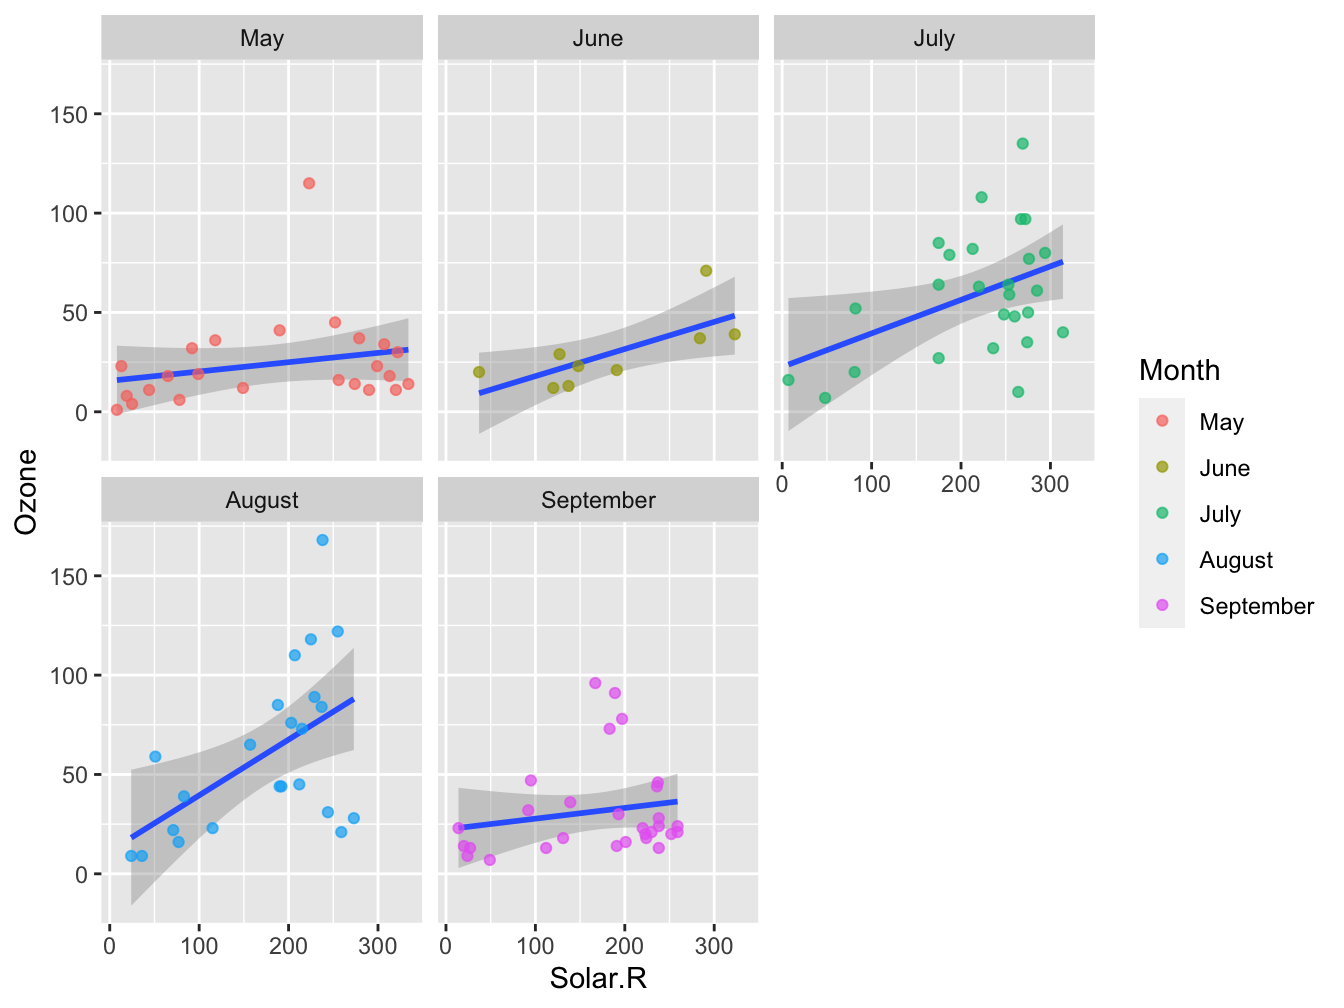
\includegraphics[width=0.8\linewidth]{davur_ebook_files/figure-latex/facetting-example-1} 

}

\caption{A facetplot - multiple similar plots split over a single nominal or ordinal variable}\label{fig:facetting-example}
\end{figure}

\begin{figure}

{\centering 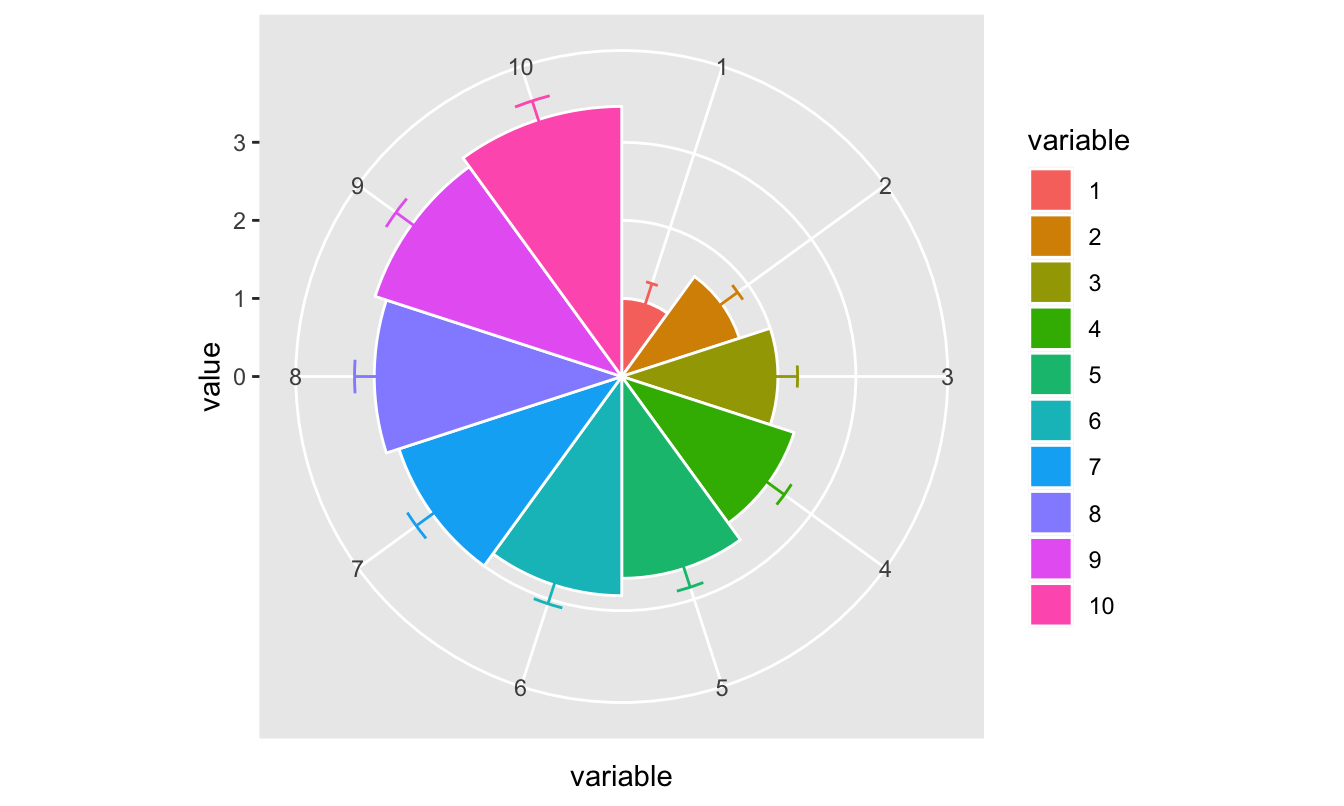
\includegraphics[width=0.8\linewidth]{davur_ebook_files/figure-latex/polarplot-1} 

}

\caption{A polar plot - the dimensions are not your normal 2d x and y}\label{fig:polarplot}
\end{figure}

\begin{figure}
\centering
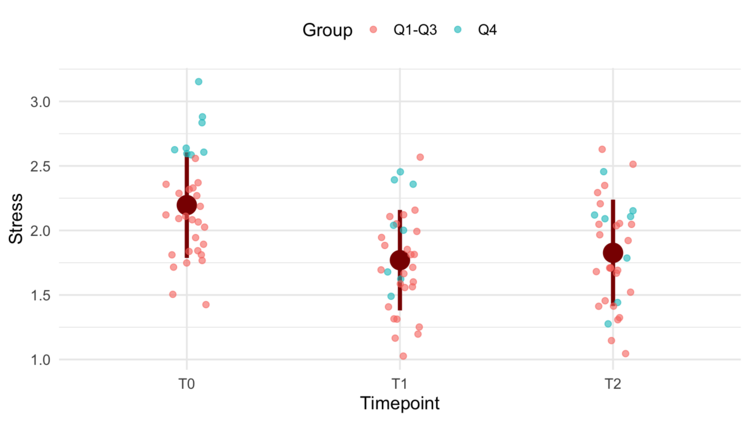
\includegraphics{figures/ptsd-jitter-5-1s.png}
\caption{A custom jitter visualization}
\end{figure}

\hypertarget{tool-2-rstudio-as-development-environment}{%
\subsection{Tool 2: RStudio as development environment}\label{tool-2-rstudio-as-development-environment}}

\begin{figure}
\centering

\includegraphics{figures/RStudioLogo.png}
\caption{RStudio logo}
\end{figure}

RStudio is a so-called Integrated Development Environment. This means it is a ``Swiss Mulitool'' for programming. With it, you manage and run code, files, documentation on the language (help pages), building different output formats.
The workbench has several panels and looks like this when you run the application.

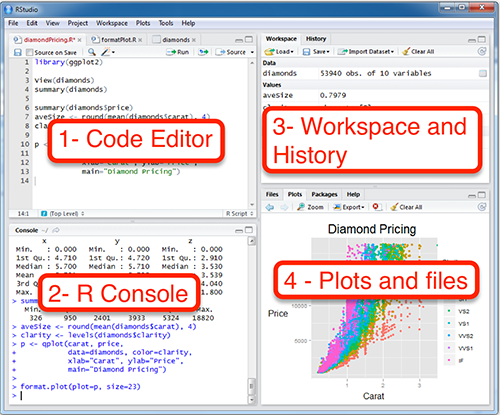
\includegraphics{figures/RStudio_screen3.png}

You primarily work with 4 panels of the workbench:

\begin{enumerate}
\def\labelenumi{\arabic{enumi}.}
\tightlist
\item
  \textbf{Code editor} where you write your scripts and RMarkdown documents: text files with code you want to execute more than once
\item
  \textbf{R console} where you execute lines of code one by one
\item
  \textbf{Environment and History} See what data you have in memory, and what you have done so far
\item
  \textbf{Plots, Help \& Files}
\end{enumerate}

You use the console to do basic calculations, try pieces of code, develop a function, or load scripts (from the code editor) into memory. On the other hand, the code editor is used to work on code that has life span longer than a few minutes: analyses you may want to repeat, or develop further in the form of scripts and RMarkdown documents.
The code editor supports many file types for viewing and editing: regular text, structured datafiles (text, csv, data files), scripts (programs), and analytical notebooks (RMarkdown).

What is nice about the \textbf{\emph{code editor}} above regular text editors such as Notepad, Wordpad, TextEdit, is that it knows about different file types and their constituting elements and helps your read, write (autocomplete, error alerts), scan and organize them by displaying these elements using coloring, font types and other visual aids.

Here is the same piece of code, which is a plain text file, in two different editors. First as plain text in the Mac TextEdit app and next in the RStudio code editor:

\begin{figure}
\centering
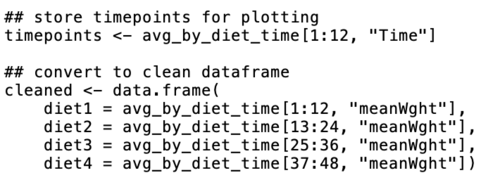
\includegraphics{figures/R_code_plain.png}
\caption{code in TextEdit}
\end{figure}

\begin{figure}
\centering
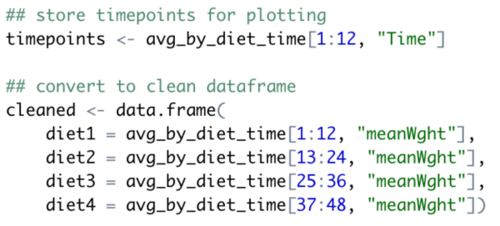
\includegraphics{figures/R_code_highlighted.png}
\caption{exact same file in RStudio editor}
\end{figure}

It is clearly visible where the code elements, numeric data and character data are within the code.

\hypertarget{tool-3-rmarkdown}{%
\subsection{Tool 3: RMarkdown}\label{tool-3-rmarkdown}}


\includegraphics{figures/markdown_logo.jpg}

In RMarkdown, you can combine regular text and figures with embedded R code that will be executed to generate a final document.

You can use it to create reports in word, pdf or web (html); create presentations (pdf or web); create entire ebooks and websites (such as this one). This entire ebook itself is written in RMarkdown!

Markdown is a very basic \textbf{\emph{markup}} language. Markup means that you use textual elements to indicate structure instead of content. RMarkdown simply is Markdown with embedded pieces of R code. Consider this piece of Markdown:

\begin{verbatim}
### Tool 3: RMarkdown

![](figures/markdown_logo.jpg)

In RMarkdown, you can combine regular text and figures with embedded R code that will be executed to generate a final document.
\end{verbatim}

The result of this snippet is the top of the current paragraph you are reading.

Here is a piece of R code we call a \textbf{\emph{code chunk}} that plots some random data in a scatter plot. In RStudio this piece of R code within (the current) RMarkdown document looks like this:

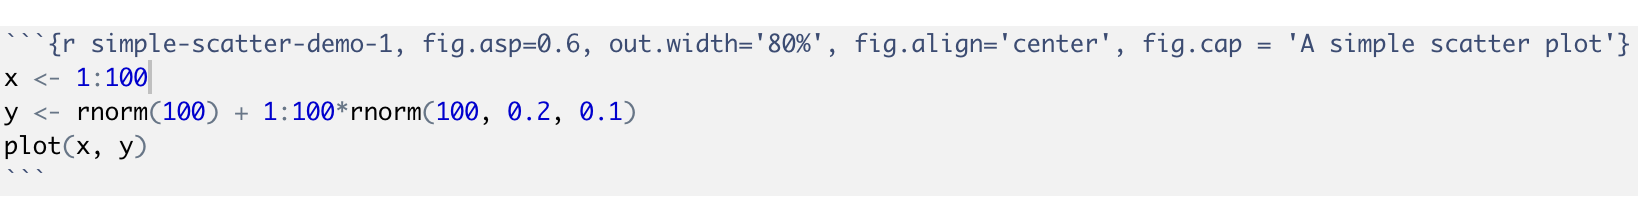
\includegraphics{figures/code_chunk.png}
Next, when I \textbf{\emph{knit}} the document into web format it results in the piece below together with its output, a scatter plot.

\begin{Shaded}
\begin{Highlighting}[]
\NormalTok{x <-}\StringTok{ }\DecValTok{1}\OperatorTok{:}\DecValTok{100}
\NormalTok{y <-}\StringTok{ }\KeywordTok{rnorm}\NormalTok{(}\DecValTok{100}\NormalTok{) }\OperatorTok{+}\StringTok{ }\DecValTok{1}\OperatorTok{:}\DecValTok{100}\OperatorTok{*}\KeywordTok{rnorm}\NormalTok{(}\DecValTok{100}\NormalTok{, }\FloatTok{0.2}\NormalTok{, }\FloatTok{0.1}\NormalTok{)}
\KeywordTok{plot}\NormalTok{(x, y)}
\end{Highlighting}
\end{Shaded}

\begin{figure}

{\centering 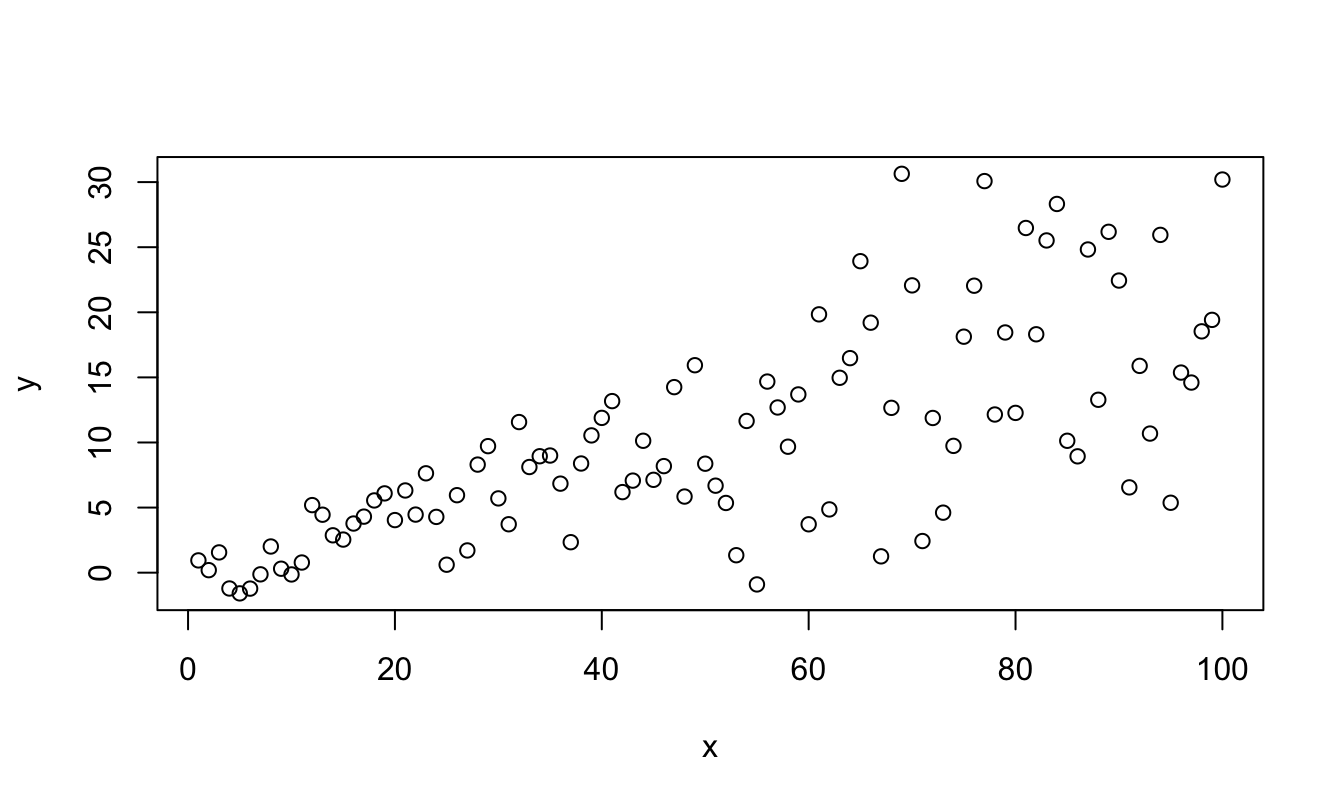
\includegraphics[width=0.8\linewidth]{davur_ebook_files/figure-latex/simple-scatter-demo-1-1} 

}

\caption{A simple scatter plot}\label{fig:simple-scatter-demo-1}
\end{figure}

RMarkdown is really basic; in fact it is translated into html, the markup language of the web, before any further processing occurs. That is why you can also embed html elements within it. Here are the most basic elements you can use in Markdown documents.

\begin{figure}
\centering
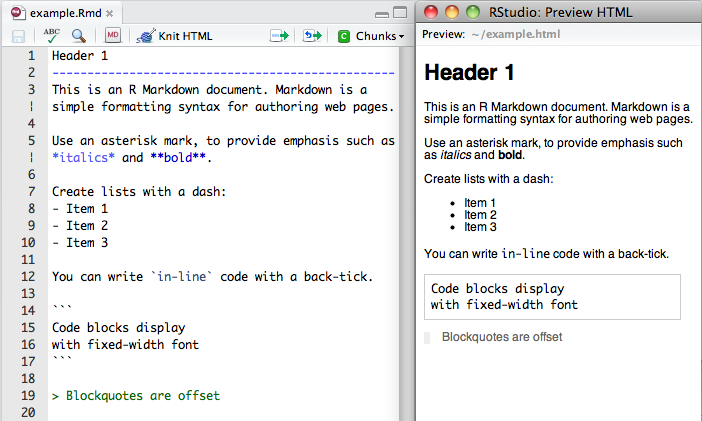
\includegraphics{figures/markdownOverview.png}
\caption{RMarkdown}
\end{figure}

Finally, it is also possible to embed Latex elements. For instance, equations can be defined in a text format. This:

\begin{verbatim}
$$d(p, q) = \sqrt{\sum_{i = 1}^{n}(q_i-p_i)^2}$$
\end{verbatim}

results in this:

\[d(p, q) = \sqrt{\sum_{i = 1}^{n}(q_i-p_i)^2}\]

Happy coding!

\hypertarget{basic-r}{%
\chapter{Basic R}\label{basic-r}}

\textbf{\emph{TO BE PORTED FROM PRESENTATION}}

\hypertarget{complex-datatypes}{%
\chapter{Complex Datatypes}\label{complex-datatypes}}

\textbf{\emph{TO BE PORTED FROM PRESENTATION}}

\hypertarget{functions}{%
\chapter{Functions}\label{functions}}

\textbf{\emph{TO BE PORTED FROM PRESENTATION}}

\hypertarget{scripting}{%
\chapter{Scripting}\label{scripting}}

\textbf{\emph{TO BE PORTED FROM PRESENTATION}}

\hypertarget{dataframe-manipulations}{%
\chapter{Dataframe manipulations}\label{dataframe-manipulations}}

\textbf{\emph{TO BE PORTED FROM PRESENTATION}}

\hypertarget{exercises}{%
\chapter{Exercises}\label{exercises}}

This chapter only contains exercises. The solutions are in the next chapter which has a numbering parallel to this one.

\hypertarget{basic-r-1}{%
\section{Basic R}\label{basic-r-1}}

\hypertarget{plotting-rules}{%
\subsection*{Plotting rules}\label{plotting-rules}}
\addcontentsline{toc}{subsection}{Plotting rules}

With all plots, take care to adhere to the rules regarding titles and other decorations. Tip: the site \href{http://www.statmethods.net/}{Quick-R} has nice detailed information with examples on the different plot types and their configuration. Especially the section \href{http://www.statmethods.net/graphs/index.html}{on plotting} is helpful for these assignments.

\hypertarget{stair-walking-and-heart-rate}{%
\subsection{Stair walking and heart rate}\label{stair-walking-and-heart-rate}}

The vectors below hold data for a staircase walking experiment. A subject of normal weight and height was asked to ascend a (long) stairs wearing a heart-rate monitor. The subjects' heart was registered for different step heights. Create a \textbf{line plot} showing the dependence of heart rate (y axis) on stair height (x axis).

\begin{Shaded}
\begin{Highlighting}[]
\CommentTok{#number of steps on the stairs}
\NormalTok{stair_height <-}\StringTok{ }\KeywordTok{c}\NormalTok{(}\DecValTok{0}\NormalTok{, }\DecValTok{5}\NormalTok{, }\DecValTok{10}\NormalTok{, }\DecValTok{15}\NormalTok{, }\DecValTok{20}\NormalTok{, }\DecValTok{25}\NormalTok{, }\DecValTok{30}\NormalTok{, }\DecValTok{35}\NormalTok{)}
\CommentTok{#heart rate after ascending the stairs}
\NormalTok{heart_rate <-}\StringTok{ }\KeywordTok{c}\NormalTok{(}\DecValTok{66}\NormalTok{, }\DecValTok{65}\NormalTok{, }\DecValTok{67}\NormalTok{, }\DecValTok{69}\NormalTok{, }\DecValTok{73}\NormalTok{, }\DecValTok{79}\NormalTok{, }\DecValTok{86}\NormalTok{, }\DecValTok{97}\NormalTok{)}
\end{Highlighting}
\end{Shaded}

\hypertarget{more-subjects}{%
\subsection{More subjects}\label{more-subjects}}

The experiment from the previous question was extended with three more subjects. One of these subjects was like the first of normal weight, whereas the two others were obese. The data are given below. Create a single \textbf{scatter plot} with connector lines between the points showing the data for all four subjects. Give the normal-weighted subjects a green line and symbol and the obese subjects a red line and symbol.\\
You can add new data series to a plot by using the \texttt{points(x,\ y)} function. Use the \texttt{ylim()} function to adjust the Y-axis range.

\begin{Shaded}
\begin{Highlighting}[]
\CommentTok{#number of steps on the stairs}
\NormalTok{stair_height <-}\StringTok{ }\KeywordTok{c}\NormalTok{(}\DecValTok{0}\NormalTok{, }\DecValTok{5}\NormalTok{, }\DecValTok{10}\NormalTok{, }\DecValTok{15}\NormalTok{, }\DecValTok{20}\NormalTok{, }\DecValTok{25}\NormalTok{, }\DecValTok{30}\NormalTok{, }\DecValTok{35}\NormalTok{)}
\CommentTok{#heart rates for subjects with normal weight}
\NormalTok{heart_rate_}\DecValTok{1}\NormalTok{ <-}\StringTok{ }\KeywordTok{c}\NormalTok{(}\DecValTok{66}\NormalTok{, }\DecValTok{65}\NormalTok{, }\DecValTok{67}\NormalTok{, }\DecValTok{69}\NormalTok{, }\DecValTok{73}\NormalTok{, }\DecValTok{79}\NormalTok{, }\DecValTok{86}\NormalTok{, }\DecValTok{97}\NormalTok{)}
\NormalTok{heart_rate_}\DecValTok{2}\NormalTok{ <-}\StringTok{ }\KeywordTok{c}\NormalTok{(}\DecValTok{61}\NormalTok{, }\DecValTok{61}\NormalTok{, }\DecValTok{63}\NormalTok{, }\DecValTok{68}\NormalTok{, }\DecValTok{74}\NormalTok{, }\DecValTok{81}\NormalTok{, }\DecValTok{89}\NormalTok{, }\DecValTok{104}\NormalTok{)}
\CommentTok{#heart rates for obese subjects}
\NormalTok{heart_rate_}\DecValTok{3}\NormalTok{ <-}\StringTok{ }\KeywordTok{c}\NormalTok{(}\DecValTok{58}\NormalTok{, }\DecValTok{60}\NormalTok{, }\DecValTok{67}\NormalTok{, }\DecValTok{71}\NormalTok{, }\DecValTok{78}\NormalTok{, }\DecValTok{89}\NormalTok{, }\DecValTok{104}\NormalTok{, }\DecValTok{121}\NormalTok{)}
\NormalTok{heart_rate_}\DecValTok{4}\NormalTok{ <-}\StringTok{ }\KeywordTok{c}\NormalTok{(}\DecValTok{69}\NormalTok{, }\DecValTok{73}\NormalTok{, }\DecValTok{77}\NormalTok{, }\DecValTok{83}\NormalTok{, }\DecValTok{88}\NormalTok{, }\DecValTok{96}\NormalTok{, }\DecValTok{102}\NormalTok{, }\DecValTok{127}\NormalTok{)}
\end{Highlighting}
\end{Shaded}

\hypertarget{chickens-on-a-diet}{%
\subsection{Chickens on a diet}\label{chickens-on-a-diet}}

The body weights of chicks were measured at birth and every second day thereafter until day 20. They were also measured on day 21. In the experiment there were four groups of chicks on different protein diets. Here are the data for the first four chicks. Chick one and two were on diet 1 and chick three and four were on diet 2. Create a single line plot showing the data for all four chicks. Give each chick its own color.

\begin{Shaded}
\begin{Highlighting}[]
\CommentTok{# chick weight data}
\NormalTok{time <-}\StringTok{ }\KeywordTok{c}\NormalTok{(}\DecValTok{0}\NormalTok{, }\DecValTok{2}\NormalTok{, }\DecValTok{4}\NormalTok{, }\DecValTok{6}\NormalTok{, }\DecValTok{8}\NormalTok{, }\DecValTok{10}\NormalTok{, }\DecValTok{12}\NormalTok{, }\DecValTok{14}\NormalTok{, }\DecValTok{16}\NormalTok{, }\DecValTok{18}\NormalTok{, }\DecValTok{20}\NormalTok{, }\DecValTok{21}\NormalTok{)}
\NormalTok{chick_}\DecValTok{1}\NormalTok{ <-}\StringTok{ }\KeywordTok{c}\NormalTok{(}\DecValTok{42}\NormalTok{, }\DecValTok{51}\NormalTok{, }\DecValTok{59}\NormalTok{, }\DecValTok{64}\NormalTok{, }\DecValTok{76}\NormalTok{, }\DecValTok{93}\NormalTok{, }\DecValTok{106}\NormalTok{, }\DecValTok{125}\NormalTok{, }\DecValTok{149}\NormalTok{, }\DecValTok{171}\NormalTok{, }\DecValTok{199}\NormalTok{, }\DecValTok{205}\NormalTok{)}
\NormalTok{chick_}\DecValTok{2}\NormalTok{ <-}\StringTok{ }\KeywordTok{c}\NormalTok{(}\DecValTok{40}\NormalTok{, }\DecValTok{49}\NormalTok{, }\DecValTok{58}\NormalTok{, }\DecValTok{72}\NormalTok{, }\DecValTok{84}\NormalTok{, }\DecValTok{103}\NormalTok{, }\DecValTok{122}\NormalTok{, }\DecValTok{138}\NormalTok{, }\DecValTok{162}\NormalTok{, }\DecValTok{187}\NormalTok{, }\DecValTok{209}\NormalTok{, }\DecValTok{215}\NormalTok{)}
\NormalTok{chick_}\DecValTok{3}\NormalTok{ <-}\StringTok{ }\KeywordTok{c}\NormalTok{(}\DecValTok{42}\NormalTok{, }\DecValTok{53}\NormalTok{, }\DecValTok{62}\NormalTok{, }\DecValTok{73}\NormalTok{, }\DecValTok{85}\NormalTok{, }\DecValTok{102}\NormalTok{, }\DecValTok{123}\NormalTok{, }\DecValTok{138}\NormalTok{, }\DecValTok{170}\NormalTok{, }\DecValTok{204}\NormalTok{, }\DecValTok{235}\NormalTok{, }\DecValTok{256}\NormalTok{)}
\NormalTok{chick_}\DecValTok{4}\NormalTok{ <-}\StringTok{ }\KeywordTok{c}\NormalTok{(}\DecValTok{41}\NormalTok{, }\DecValTok{49}\NormalTok{, }\DecValTok{61}\NormalTok{, }\DecValTok{74}\NormalTok{, }\DecValTok{98}\NormalTok{, }\DecValTok{109}\NormalTok{, }\DecValTok{128}\NormalTok{, }\DecValTok{154}\NormalTok{, }\DecValTok{192}\NormalTok{, }\DecValTok{232}\NormalTok{, }\DecValTok{280}\NormalTok{, }\DecValTok{290}\NormalTok{)}
\end{Highlighting}
\end{Shaded}

\hypertarget{chicken-bar-plot}{%
\subsection{Chicken bar plot}\label{chicken-bar-plot}}

With the data from the previous question, create a bar plot of the maximum weights of the chicks.

\hypertarget{discoveries}{%
\subsection{Discoveries}\label{discoveries}}

The R language comes with a wealth of datasets for you to use as practice materials. We will see several of these. One of these datasets is The Time-Series dataset called \texttt{discoveries} holding the numbers of ``great'' inventions and scientific discoveries in each year from 1860 to 1959. Type its name in the console to see it. Create plot(s) answering these questions:

\textbf{A}

What is the number of discoveries per year? Use the \texttt{barplot()} and \texttt{table()} functions for this.

\textbf{B}

What is the 5-number summary of discoveries per year?

\textbf{C}

What is the trend over time for the numbers of discoveries per year?

PS: This is actually not a simple vector but a vector with some time-related attributes. It is called a Time-Series (a \texttt{ts} class), but this does not really matter for this assignment.

\hypertarget{lung-cancer}{%
\subsection{Lung cancer}\label{lung-cancer}}

The R datasets package has three related timeseries datasets relating to lung cancer deaths. These are \texttt{ldeaths}, \texttt{mdeaths} and \texttt{fdeaths} for total, male and female deaths respectively. Create a line plot showing the monthly mortality holding all three of these datasets. Use the \texttt{legend()} function to add a legend to the plot, as demonstrated in this example:

\begin{Shaded}
\begin{Highlighting}[]
\NormalTok{t <-}\StringTok{ }\DecValTok{1}\OperatorTok{:}\DecValTok{5}
\NormalTok{y1 <-}\StringTok{ }\KeywordTok{c}\NormalTok{(}\DecValTok{2}\NormalTok{, }\DecValTok{3}\NormalTok{, }\DecValTok{5}\NormalTok{, }\DecValTok{4}\NormalTok{, }\DecValTok{6}\NormalTok{)}
\NormalTok{y2 <-}\StringTok{ }\KeywordTok{c}\NormalTok{(}\DecValTok{1}\NormalTok{, }\DecValTok{3}\NormalTok{, }\DecValTok{4}\NormalTok{, }\DecValTok{5}\NormalTok{, }\DecValTok{7}\NormalTok{)}
\KeywordTok{plot}\NormalTok{(t, y1, }\DataTypeTok{type =} \StringTok{"b"}\NormalTok{, }\DataTypeTok{ylab =} \StringTok{"response"}\NormalTok{, }\DataTypeTok{ylim =} \KeywordTok{c}\NormalTok{(}\DecValTok{0}\NormalTok{, }\DecValTok{8}\NormalTok{))}
\KeywordTok{points}\NormalTok{(t, y2, }\DataTypeTok{col =} \StringTok{"blue"}\NormalTok{, }\DataTypeTok{type =} \StringTok{"b"}\NormalTok{)}
\KeywordTok{legend}\NormalTok{(}\StringTok{"topleft"}\NormalTok{, }\DataTypeTok{legend =} \KeywordTok{c}\NormalTok{(}\StringTok{"series 1"}\NormalTok{, }\StringTok{"series 2"}\NormalTok{), }\DataTypeTok{col =} \KeywordTok{c}\NormalTok{(}\StringTok{"black"}\NormalTok{, }\StringTok{"blue"}\NormalTok{), }\DataTypeTok{pch =} \DecValTok{1}\NormalTok{, }\DataTypeTok{lty =} \DecValTok{1}\NormalTok{)}
\end{Highlighting}
\end{Shaded}

\begin{center}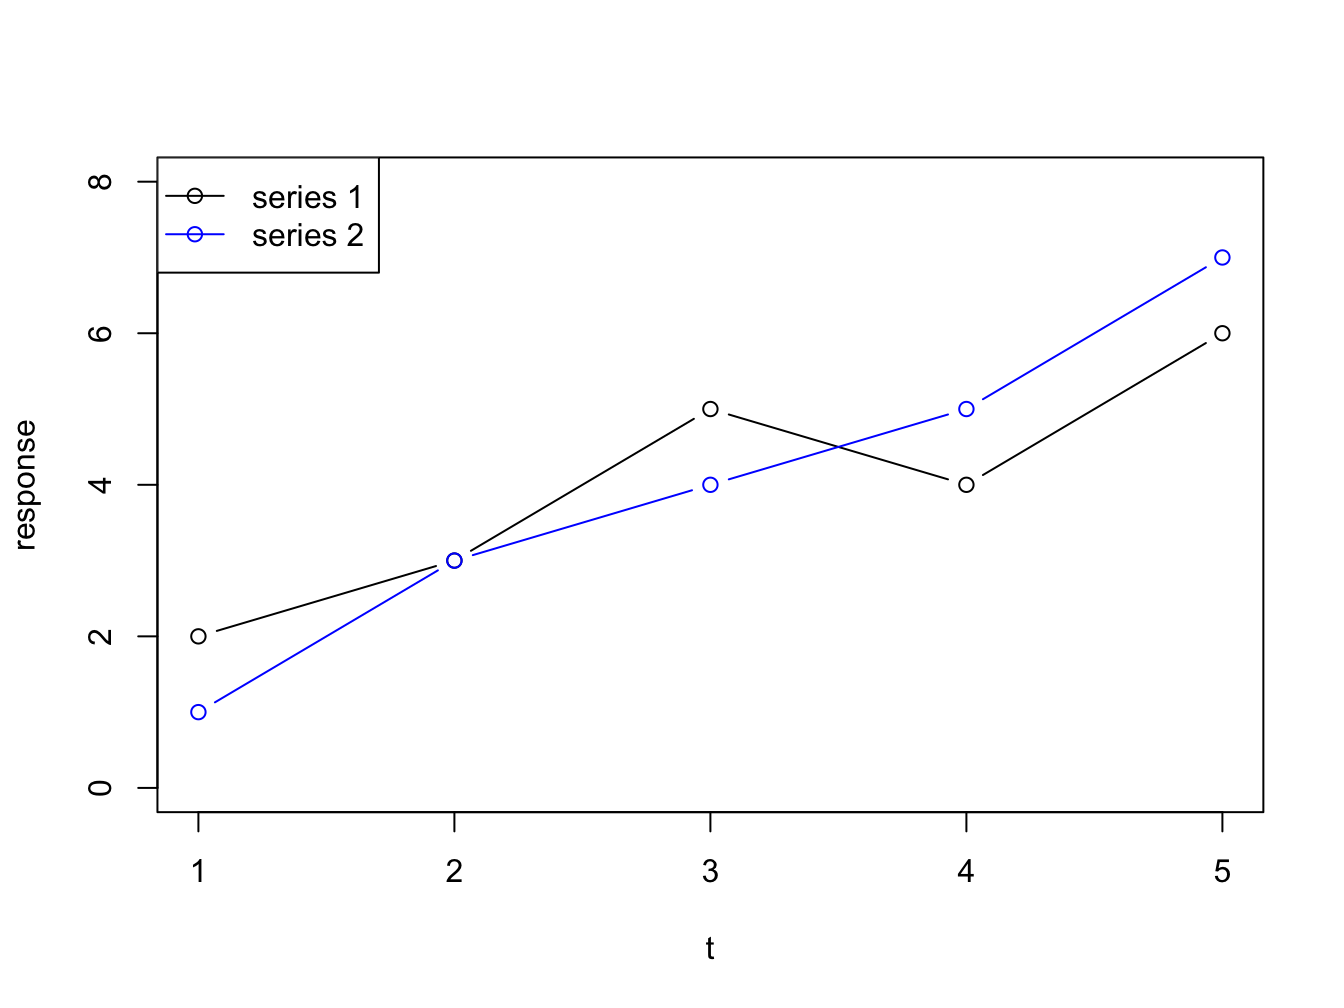
\includegraphics[width=0.8\linewidth]{davur_ebook_files/figure-latex/legend-demo-1} \end{center}

\textbf{A}

Create the mentioned line plot. Do you see trends and/or patterns and if so, can you explain these?

\textbf{B}

Create a combined boxplot of the three time-series. Are there outliers? If so, can you figure out when this occurred?

\hypertarget{complex-datatypes-1}{%
\section{Complex datatypes}\label{complex-datatypes-1}}

This section serves you some datatype challenges.

\hypertarget{creating-factors}{%
\subsection{Creating factors}\label{creating-factors}}

\textbf{A}

Given this vector:

\begin{Shaded}
\begin{Highlighting}[]
\NormalTok{animal_risk <-}\StringTok{ }\KeywordTok{c}\NormalTok{(}\DecValTok{2}\NormalTok{, }\DecValTok{4}\NormalTok{, }\DecValTok{1}\NormalTok{, }\DecValTok{1}\NormalTok{, }\DecValTok{2}\NormalTok{, }\DecValTok{4}\NormalTok{, }\DecValTok{1}\NormalTok{, }\DecValTok{4}\NormalTok{, }\DecValTok{1}\NormalTok{, }\DecValTok{1}\NormalTok{, }\DecValTok{2}\NormalTok{, }\DecValTok{1}\NormalTok{)}
\end{Highlighting}
\end{Shaded}

and these possible levels:
1: harmless
2: risky
3: dangerous
4: deadly

Create a factor from this data and then barplot the result.

\textbf{B}

Given this data, a simulation of wealth distribution of ``poor'', ``middle class'', ``wealthy'' "rich:

\begin{Shaded}
\begin{Highlighting}[]
\KeywordTok{set.seed}\NormalTok{(}\DecValTok{1234}\NormalTok{)}
\NormalTok{wealth_male <-}\StringTok{ }\KeywordTok{sample}\NormalTok{(}\DataTypeTok{x =}\NormalTok{ letters[}\DecValTok{1}\OperatorTok{:}\DecValTok{4}\NormalTok{], }
                 \DataTypeTok{size =} \DecValTok{1000}\NormalTok{,}
                 \DataTypeTok{replace=} \OtherTok{TRUE}\NormalTok{, }
                 \DataTypeTok{prob =} \KeywordTok{c}\NormalTok{(}\FloatTok{0.7}\NormalTok{, }\FloatTok{0.17}\NormalTok{, }\FloatTok{0.12}\NormalTok{, }\FloatTok{0.01}\NormalTok{))}
\NormalTok{wealth_female <-}\StringTok{ }\KeywordTok{sample}\NormalTok{(}\DataTypeTok{x =}\NormalTok{ letters[}\DecValTok{1}\OperatorTok{:}\DecValTok{4}\NormalTok{], }
                 \DataTypeTok{size =} \DecValTok{1000}\NormalTok{,}
                 \DataTypeTok{replace=} \OtherTok{TRUE}\NormalTok{, }
                 \DataTypeTok{prob =} \KeywordTok{c}\NormalTok{(}\FloatTok{0.8}\NormalTok{, }\FloatTok{0.15}\NormalTok{, }\FloatTok{0.497}\NormalTok{, }\FloatTok{0.003}\NormalTok{))}
\end{Highlighting}
\end{Shaded}

Create a factor from these two and report the cumulative percentage of its individual levels starting at the most abundant level, combined for male and female. Hint: use \texttt{table()} and \texttt{prop.table()}.

Next, create a side-by-side barplot of this data. Don't forget the legend!

\hypertarget{a-dictionary-with-a-named-vector}{%
\subsection{A dictionary with a named vector}\label{a-dictionary-with-a-named-vector}}

Almost all programming languages know the (hash)map / dictionary data structure storing so-called ``key-and-value'' pairs. They make it possible to ``look up'' the value belonging to a ``key''. That is where the term dictionary comes from. A dictionary holds keys (the words) and their meaning (values). R does not have a dictionary type but you could make a dict-like structure using a \textbf{\emph{vector with named elements}}. Here follows an example.

If I wanted to create and use a DNA codon translation table, and use it to translate a piece of DNA, I could do something like what is shown below (there are only 4 of the 64 codons included). See if you can figure out what is going on there

\begin{Shaded}
\begin{Highlighting}[]
\CommentTok{## define codon table as named vector}
\NormalTok{codons <-}\StringTok{ }\KeywordTok{c}\NormalTok{(}\StringTok{"Gly"}\NormalTok{, }\StringTok{"Pro"}\NormalTok{, }\StringTok{"Lys"}\NormalTok{, }\StringTok{"Ser"}\NormalTok{)}
\KeywordTok{names}\NormalTok{(codons) <-}\StringTok{ }\KeywordTok{c}\NormalTok{(}\StringTok{"GGA"}\NormalTok{, }\StringTok{"CCU"}\NormalTok{, }\StringTok{"AAA"}\NormalTok{, }\StringTok{"AGU"}\NormalTok{)}

\CommentTok{## the DNA to translate}
\NormalTok{my_DNA <-}\StringTok{ "GGACCUAAAAGU"}
\NormalTok{my_prot <-}\StringTok{ ""}
\CommentTok{## iterate the DNA and take only every position}
\ControlFlowTok{for}\NormalTok{ (i }\ControlFlowTok{in} \KeywordTok{seq}\NormalTok{(}\DecValTok{1}\NormalTok{, }\KeywordTok{nchar}\NormalTok{(my_DNA), }\DataTypeTok{by=}\DecValTok{3}\NormalTok{)) \{}
\NormalTok{    codon <-}\StringTok{ }\KeywordTok{substr}\NormalTok{(my_DNA, i, i}\OperatorTok{+}\DecValTok{2}\NormalTok{);}
\NormalTok{    my_prot <-}\StringTok{ }\KeywordTok{paste}\NormalTok{(my_prot, codons[codon])}
\NormalTok{\}}
\KeywordTok{print}\NormalTok{(my_prot)}
\end{Highlighting}
\end{Shaded}

\begin{verbatim}
## [1] " Gly Pro Lys Ser"
\end{verbatim}

\textbf{A}

Make a modified copy of this code chunk in such a way that no spaces are present between the amino acid residues (use help on \texttt{paste()} to figure this out) and that single-letter codes of amino acids are used instead of three-letter codes.

\textbf{B}

\textbf{{[}Challenge{]}} Here is a vector called \texttt{nuc\_weights}. It holds the weights for the nucleotides A, C, G and U respectively. Make it a named vector, iterate \texttt{my\_DNA} from the above code chunk and calculate its molecular weight.

\begin{Shaded}
\begin{Highlighting}[]
\NormalTok{nuc_weights <-}\StringTok{ }\KeywordTok{c}\NormalTok{(}\FloatTok{491.2}\NormalTok{, }\FloatTok{467.2}\NormalTok{, }\FloatTok{507.2}\NormalTok{, }\FloatTok{482.2}\NormalTok{)}
\end{Highlighting}
\end{Shaded}

\hypertarget{airquality}{%
\subsection{airquality}\label{airquality}}

The \texttt{airquality} dataset is also one of the datasets included in the \texttt{datasets} package. We'll explore this for a few questions.

\textbf{A}

Create a scatterplot of Temperature as a function of Solar radiation. Is there, as you might naively expect, a strong correlation? You could use \texttt{cor.test()} to find out. Add a linear model using \texttt{lm()} to extend your plot.

\textbf{B}

Create a boxplot-series of \texttt{Temp} as a function of \texttt{Month} (use \texttt{?boxplot} to find out how this works). What appears to be the warmest month?

\textbf{C}

What date (day/month) has the lowest recorded temperature? Which the highest? Please give temperature values in Celsius, not Fahrenheit! (Yes, this is an extra challenge!)

\textbf{D}

Create a histogram of the wind speeds, and add a thick blue vertical line for the value of the mean and a fat red line for the median (use \texttt{abline()} for this).

\textbf{E}

Use the \texttt{pairs()} function with argument \texttt{panel\ =\ panel.smooth} to plot all pairwise correlations between Ozone, Solar radiation, Wind and Temperature. Which pair shows the strongest correlation in your opinion? Verify this using the \texttt{cor()} function after removing incomplete cases. Create a separate well annotated scatterplot of this pair.

\hypertarget{bird-observations}{%
\subsection{Bird observations}\label{bird-observations}}

You will explore a bird observation dataset, downloaded from \href{http://goldengateaudubon.org/birding-resources/observations/}{GOLDEN GATE AUDUBON SOCIETY}. This file lists bird observations collected by this bird monitoring group in the San Francisco Bay Area. I already cleaned it a bit and placed it here: \url{data/Observations-Data-2014.csv}.

You can download it as follows:

\begin{Shaded}
\begin{Highlighting}[]
\NormalTok{file_name <-}\StringTok{ "Observations-Data-2014.csv"}
\NormalTok{remote_url <-}\StringTok{ }\KeywordTok{paste0}\NormalTok{(}\StringTok{"https://raw.githubusercontent.com/MichielNoback/davur1_gitbook/master/data/"}\NormalTok{, file_name)}

\KeywordTok{download.file}\NormalTok{(}\DataTypeTok{url =}\NormalTok{ remote_url, }\DataTypeTok{destfile =}\NormalTok{ file_name)}
\end{Highlighting}
\end{Shaded}

Load the observation data into R and assign it to a variable called \texttt{bird\_obs}.

From here on, it is assumed that you have the dataframe \texttt{bird\_obs} loaded. This series of exercises deals with cleaning and transforming data, and exploring a cleaned dataset using basic plotting techniques and descriptive statistics.

\textbf{A}

First, explore the raw data as they are.

\begin{itemize}
\tightlist
\item
  What data on bird observations were recorded (i.e.~what kind of variables do you have)?
\item
  What did R do to the original column names?
\item
  Are all column names clear to you?
\end{itemize}

\textbf{B}

How many bird observations were recorded?

\textbf{C}

The column holding observation ``Number'' is actually not a number. Into what type has R converted it?

\textbf{D}

Convert the ``Number'' column into an integer column using \texttt{as.integer()}, but assign it to a new column called ``Count'' (i.e.~do not overwrite the original values). Compare the first 50 values or so of these two columns. What happened to the data? Is this OK?

\textbf{E}

The previous question has shown that converting factors to numbers is a bit dangerous. It is often easiest to convert characters to numbers. The best way to do this is by using the \texttt{as.is\ =\ c(\textless{}column\ indices\textgreater{})} argument for the \texttt{read.table()} function.

So, which columns should be loaded as real factor data and which as plain character data? Use \texttt{read.table()} and the \texttt{as.is} argument to reload the data, and then transform the \texttt{Number} column to integer again as \texttt{Count}.

\textbf{F}

Compare the first 50 values of the Number and Count columns again. Has the conversion succeeded? How many \texttt{Number} values could not be transformed into an integer value? Hint: use \texttt{is.na()}

\textbf{G}

Explore the sighting counts:

\begin{itemize}
\tightlist
\item
  What is the maximum number of birds in a single sighting? (Use max() and which() or is.na() to solve this)
\item
  What is the mean sighting count
\item
  What is the median of the sighting count
\end{itemize}

\textbf{H}

Is the \texttt{Count} variable a normal distributed value? You can use \texttt{hist(...)}, \texttt{table()} or \texttt{plot(density(...))} to explore this further.

\textbf{I}

Explore the species constitution:

\begin{itemize}
\tightlist
\item
  How many different species were recorded?
\item
  How many genera do they constitute?
\item
  What species from the genus ``Puffinus'' have been observed?
\end{itemize}

Hint: use the function \texttt{unique()} here.

\textbf{J {[}Challenge{]}}\\
This is a challenge exercise for those who like to grind their brains! Think of a strategy to ``rescue'' the NAs that appear after transforming ``Number'' to ``Count''. Hint: use \texttt{gsub()} or\texttt{grep()}

\hypertarget{regular-expressions}{%
\section{Regular Expressions}\label{regular-expressions}}

\hypertarget{restriction-enzymes}{%
\subsection{Restriction enzymes}\label{restriction-enzymes}}

\textbf{A}

The restriction enzyme PacI has the recognition sequence ``TTAATTAA''. Define (at least) three alternative regex patterns that will catch these sites.

\textbf{B}

The restriction enzyme SfiI has the recognition sequence ``GGCCNNNNNGGCC''. Define (at least) three alternative regex patterns that will catch these sites.

\hypertarget{prosite-patterns}{%
\subsection{Prosite Patterns}\label{prosite-patterns}}

\textbf{A}

The Prosite pattern PS00211 (ABC-transporter-1; \url{https://prosite.expasy.org/PS00211}) has the pattern:\\
``{[}LIVMFYC{]}-{[}SA{]}-{[}SAPGLVFYKQH{]}-G-{[}DENQMW{]}-{[}KRQASPCLIMFW{]}-{[}KRNQSTAVM{]}-{[}KRACLVM{]}-{[}LIVMFYPAN{]}-\{PHY\}-{[}LIVMFW{]}-{[}SAGCLIVP{]}-\{FYWHP\}-\{KRHP\}-{[}LIVMFYWSTA{]}.''
Translate it into a regex pattern. Info on the syntax is here: \url{https://prosite.expasy.org/prosuser.html\#conv_pa}

\textbf{B}

The Prosite pattern PS00018 (EF-hand calcium-binding domain; \url{https://prosite.expasy.org/PS00018}) has the pattern:
``D-\{W\}-{[}DNS{]}-\{ILVFYW\}-{[}DENSTG{]}-{[}DNQGHRK{]}-\{GP\}-{[}LIVMC{]}-{[}DENQSTAGC{]}-x(2)- {[}DE{]}-{[}LIVMFYW{]}.''
Translate it into a regex pattern.

You could exercise more by simply browsing Prosite. Test your pattern by fetching the proteins referred to within the Prosite pattern details page.

\hypertarget{fasta-headers}{%
\subsection{Fasta Headers}\label{fasta-headers}}

The fasta sequence format is a very common sequence file format used in molecular biology.
It looks like this (I omitted most of the actual protein sequences for better representation):

\begin{verbatim}
>gi|21595364|gb|AAH32336.1| FHIT protein [Homo sapiens]
MSFRFGQHLIK...ALRVYFQ
>gi|15215093|gb|AAH12662.1| Fhit protein [Mus musculus]
MSFRFGQHLIK...RVYFQA
>gi|151554847|gb|AAI47994.1| FHIT protein [Bos taurus]
MSFRFGQHLIK...LRVYFQ
\end{verbatim}

As you can see there are several distinct elements within the Fasta \textbf{\emph{header}} which is the description line above the actual sequence: one or more database identification strings, a protein description or name and an organism name. Study the format - we are going to extract some elements from these fasta headers using the \texttt{stringr} package. Install it if you don't have it yet.

Here is a small example:

\begin{Shaded}
\begin{Highlighting}[]
\KeywordTok{library}\NormalTok{(stringr)}
\NormalTok{hinfII_re <-}\StringTok{ "GA[GATC]TC"}
\NormalTok{sequences <-}\StringTok{ }\KeywordTok{c}\NormalTok{(}\StringTok{"GGGAATCC"}\NormalTok{, }\StringTok{"TCGATTCGC"}\NormalTok{, }\StringTok{"ACGAGTCTA"}\NormalTok{)}
\KeywordTok{str_extract}\NormalTok{(}\DataTypeTok{string =}\NormalTok{ sequences,}
            \DataTypeTok{pattern =}\NormalTok{ hinfII_re)}
\end{Highlighting}
\end{Shaded}

\begin{verbatim}
## [1] "GAATC" "GATTC" "GAGTC"
\end{verbatim}

Function \texttt{str\_extract()} simply extracts the exact match of your regex (shown above). On the other hand, function \texttt{str\_match()} supports \textbf{\emph{grouping capture}} through bounding parentheses:

\begin{Shaded}
\begin{Highlighting}[]
\NormalTok{phones <-}\StringTok{ }\KeywordTok{c}\NormalTok{(}\StringTok{"+31-6-23415239"}\NormalTok{, }\StringTok{"+49-51-55523146"}\NormalTok{, }\StringTok{"+31-50-5956566"}\NormalTok{)}
\NormalTok{phones_re <-}\StringTok{ "}\CharTok{\textbackslash{}\textbackslash{}}\StringTok{+(}\CharTok{\textbackslash{}\textbackslash{}}\StringTok{d\{2\})-(}\CharTok{\textbackslash{}\textbackslash{}}\StringTok{d\{1,2\})"} \CommentTok{#matching country codes and area codes}
\NormalTok{matches <-}\StringTok{ }\KeywordTok{str_match}\NormalTok{(phones, phones_re) }
\NormalTok{matches}
\end{Highlighting}
\end{Shaded}

\begin{verbatim}
##      [,1]     [,2] [,3]
## [1,] "+31-6"  "31" "6" 
## [2,] "+49-51" "49" "51"
## [3,] "+31-50" "31" "50"
\end{verbatim}

Thus, each set of parentheses will yield a column in the returned matrix. Simply use its column index to get that result set:

\begin{Shaded}
\begin{Highlighting}[]
\NormalTok{matches[, }\DecValTok{2}\NormalTok{] }\CommentTok{##the country codes}
\end{Highlighting}
\end{Shaded}

\begin{verbatim}
## [1] "31" "49" "31"
\end{verbatim}

Now, given the fasta headers in \url{./data/fasta_headers.txt}
which you can simply load into a character vector using \texttt{readLines()}, extract the following.

\textbf{A}

\begin{itemize}
\tightlist
\item
  Extract all complete organism names.\\
\item
  Extract all species-level organism names (omitting subspecies and strains etc).
\end{itemize}

\textbf{B}

Extract all \textbf{\emph{first}} database identifiers. So in this header element \texttt{\textgreater{}gi\textbar{}224017144\textbar{}gb\textbar{}EEF75156.1\textbar{}} you should extract only \texttt{gi\textbar{}224017144}

\textbf{C}

Extract all protein names/descriptions.

\hypertarget{scripting-1}{%
\section{Scripting}\label{scripting-1}}

This section serves you some exercises that will help you improve your function-writing skills.

\hypertarget{illegal-reproductions}{%
\subsection{Illegal reproductions}\label{illegal-reproductions}}

As an exercise, you will re-invent the wheel here for some statistical functions.

\hypertarget{the-mean}{%
\subsubsection*{The mean}\label{the-mean}}
\addcontentsline{toc}{subsubsection}{The mean}

Create a function, \texttt{my\_mean()}, that duplicates the R function \texttt{mean()}, i.e.~calculates and returns the mean of a vector of numbers, without actually using \texttt{mean()}.

\hypertarget{standard-deviation}{%
\subsubsection*{Standard deviation}\label{standard-deviation}}
\addcontentsline{toc}{subsubsection}{Standard deviation}

Create a function, \texttt{my\_sd()}, that duplicates the R function \texttt{sd()}, i.e.~calculates and returns the standard deviation of a vector of numbers, without actually using \texttt{sd()}.

\hypertarget{median}{%
\subsubsection*{Median}\label{median}}
\addcontentsline{toc}{subsubsection}{Median}

\textbf{{[}Challenge{]}} Create a function, \texttt{my\_median()}, that duplicates the R function \texttt{median()}, i.e.~calculates and returns the median of a vector of numbers. This is actually a bit harder than you might expect. Hint: use the \texttt{sort()} function.

\hypertarget{interquantile-ranges}{%
\subsection{Interquantile ranges}\label{interquantile-ranges}}

Create a function that will calculate a custom ``interquantile range''. The function should accept three arguments: a numeric vector, a lower quantile and an upper quantile. It should return the difference (range) between these two quantile values. The lower quantile should default to 0 and the higher to 1, thus returning \texttt{max(x)} minus \texttt{min(x)}. The function therefore has this ``signature'':

\begin{Shaded}
\begin{Highlighting}[]
\NormalTok{interquantile_range <-}\StringTok{ }\ControlFlowTok{function}\NormalTok{(x, }\DataTypeTok{lower =} \DecValTok{0}\NormalTok{, }\DataTypeTok{higher =} \DecValTok{100}\NormalTok{) \{\}}
\end{Highlighting}
\end{Shaded}

Perform some tests on the arguments to make a robust method: are all arguments numeric?

To test you method, you can compare \texttt{interquantile\_range(some\_vector,\ 0.25,\ 0.75)} with \texttt{IQR(some\_vector)} - they should be the same.

\hypertarget{vector-distance}{%
\subsection{Vector distance}\label{vector-distance}}

Create a function, \texttt{distance(p,\ q)}, that will calculate and return the Euclidean distance between two vectors of equal length. A numeric vector can be seen as a point in multidimensional space. Euclidean distance is defined as

\[d(p, q) = \sqrt{\sum_{i = 1}^{n}(q_i-p_i)^2}\]
Where \emph{p} and \emph{q} are the two vectors and \emph{n} the length of the two vectors.\\
You should first perform a check whether the two vectors are of equal length and both of type \texttt{numeric} or \texttt{integer}. If not, the function should abort with an appropriate error message.

\hypertarget{other-distance-measures}{%
\subsubsection*{Other distance measures}\label{other-distance-measures}}
\addcontentsline{toc}{subsubsection}{Other distance measures}

Extend the function of the previous assignment in such a way that a third argument is accepted, \texttt{method\ =}, which defaults to ``euclidean''. Other possible distance measures are ``Manhattan'' (same as ``city block'' and ``taxicab'') and Pearson correlation. Look the equations for these up in Wikipedia or some other place.

\hypertarget{gc-percentage-of-dna}{%
\subsection{G/C percentage of DNA}\label{gc-percentage-of-dna}}

\textbf{{[}Challenge XL{]}} Create a function, \texttt{GC\_perc()}, that calculates and returns the GC percentage of a DNA or RNA sequence. Accept as input a sequence and a flag -\texttt{strict}- indicating whether other characters are accepted than core DNA/RNA (GATUC). If \texttt{strict\ =\ FALSE}, the percentage of other characters should be reported using a \texttt{warning()} call. If \texttt{strict\ =\ TRUE}, the function should terminate with an error message. Use \texttt{stop()} for this. \texttt{strict} should default to \texttt{TRUE}. NOTE, usage of \texttt{strict} can complicate things, so start with the core functionality!
You can use \texttt{strsplit()} or \texttt{substr()} to get hold of individual sequence characters.

\hypertarget{function-apply-and-its-relatives}{%
\section{\texorpdfstring{Function \texttt{apply} and its relatives}{Function apply and its relatives}}\label{function-apply-and-its-relatives}}

In this section you will encounter some exercises revolving around the different flavors of apply.

\hypertarget{whale-selenium}{%
\subsection{Whale selenium}\label{whale-selenium}}

On the course website under \href{https://michielnoback.github.io/bincourses/course_contents/davur/resources.html}{Resources} you will find a link to file \texttt{whale\_selenium.txt}. You could download it into your working directory manually or use \texttt{download.file()} to obtain it. However, there is a third way to get its contents without actually downloading it as a local copy. You can read it directly using \texttt{read.table()} as shown here.

\begin{Shaded}
\begin{Highlighting}[]
\NormalTok{whale_sel_url <-}\StringTok{ "https://raw.githubusercontent.com/MichielNoback/davur1/gh-pages/exercises/data/whale_selenium.txt"}
\NormalTok{whale_selenium <-}\StringTok{ }\KeywordTok{read.table}\NormalTok{(whale_sel_url,}
    \DataTypeTok{header =}\NormalTok{ T,}
    \DataTypeTok{row.names =} \DecValTok{1}\NormalTok{)}
\end{Highlighting}
\end{Shaded}

Note: when you are going to load a file many times it is probably better to store a local copy.

\textbf{A}

Report the means of both columns using \texttt{apply()}.

\textbf{B}

Report the standard deviation of both columns, using \texttt{apply()}

\textbf{C}

Report the standard error of the mean of both columns, using \texttt{apply()} The SEM is calculated as \[\frac{sd}{\sqrt{n}}\] where \(sd\) is the sample standard deviation and \(n\) the number of measurements. You should create the function calculating this statistic yourself.

\textbf{D}

Using \texttt{apply()}, calculate the ratio of \(Se_{tooth} / Se_{liver}\) and attach it to the \texttt{whale\_selenium} dataframe as column \texttt{ratio}. Create a histogram of this ratio.

\textbf{E}

Using \texttt{print()} and \texttt{paste()}, report the mean and the standard deviation of the ratio column, but do this with an inline expression, e.g.~an expression embedded in the R markdown paragraph text.

\hypertarget{chickweight}{%
\subsection{ChickWeight}\label{chickweight}}

This exercise revolves around the \texttt{ChickWeight} dataset of the built-in \texttt{datasets} package.

\textbf{A}

Report the number of chickens used in the experiment.

\textbf{B}

Use \texttt{aggregate()} to get the mean weight of the chickens for the different Diets.

\textbf{C}

Use \texttt{coplot()} to plot a panel with weight as function of Time, split over Diet.

\textbf{D}

Add a column called \texttt{weight\_gain} to the dataframe holding values for the weight gain since the last measurement. Take special care with rows marking the boundaries between individual chickens! You could consider using a traditional for loop here.
In the next course, we'll see a more efficient way of doing this.

\textbf{E}

Split the \texttt{weight\_gain} column on Diet and report the mean, median and standard deviation for each diet.
If you were not successful in the previous question, load and attach the data from file \texttt{ChickWeight\_weight\_gain.Rdata} downloadable from \url{https://github.com/MichielNoback/davur1_gitbook/raw/master/data/ChickWeight_weight_gain.Rdata}. You can use this code chunk for downloading and loading the data into variable \texttt{stored\_weight\_gain}. Don't forget to attach the column to the data frame!

\begin{Shaded}
\begin{Highlighting}[]
\NormalTok{local_file <-}\StringTok{ "ChickWeight_weight_gain.Rdata"}
\KeywordTok{download.file}\NormalTok{(}\KeywordTok{paste0}\NormalTok{(}\StringTok{"https://github.com/MichielNoback/davur1_gitbook/raw/master/data/"}\NormalTok{, local_file), local_file)}
\KeywordTok{load}\NormalTok{(local_file)}
\end{Highlighting}
\end{Shaded}

\textbf{F}

Create a (single-panel) boxplot for weight gain, split over Diet. Hint: read the \texttt{boxplot()} help page!

\hypertarget{food-constituents}{%
\subsection{Food constituents}\label{food-constituents}}

The \href{https://raw.githubusercontent.com/MichielNoback/davur1_gitbook/master/data/food_constituents.txt}{food constituents dataset} holds information on ingredients for different foods. Individual foods are simply marked with an id.

\textbf{A}

Load the data and report the different food categories (\texttt{Type}). Also report the numbers of entries for each Type.

\textbf{B}

What is the mean energy content of chocolate foods?

\textbf{C}

What is the food category with the highest mean fat content?

\textbf{D}

What food category has the highest mean energy content, and which has the lowest?

\textbf{E}

\textbf{{[}Challenge{]}} Create a boxplot showing the difference in sugar content between drink and solid food.

\textbf{F}

Assuming both unsaturated fats and sugar are bad for you, what food category do you consider the worst? Think of a means to answer this, explain it and carry it out.

\hypertarget{bird-observations-revisited}{%
\subsection{Bird observations revisited}\label{bird-observations-revisited}}

This exercise revisits the bird observations dataset. You can download it \href{data/Observations-Data-2014.csv}{here}. (Re)load the dataset.

\textbf{A}

Report the number of observations per \texttt{County}. Use both a textual as a barplot representation. With the barplot, you should order the bars according to observation numbers.

\textbf{B}

Report the number of observations per \texttt{Observer.1} but only for observers with more than 10 observations, ordered from high to low observation count. Use \texttt{order()} to achieve this.

\textbf{C}

Which observer has the highest number of observations listed (and how many is that)?

\textbf{D}

Report the different observed species (using \texttt{Common.name}) for each genus. \textbf{{[}Challenge{]}} Report only the 5 Genera with the highest number of observed species.

\textbf{E}

\textbf{{[}Challenge{]}} Create a Dataframe holding the number of birds per day (use Date.start) and plot it with date on the x-axis and number of birds on the y-axis. Hint: use \texttt{as.Date()} to convert the character date to a real date field. See this page how you can do that \href{http://www.statmethods.net/input/dates.html}{Date Values}.

\hypertarget{exercise-solutions}{%
\chapter{Exercise solutions}\label{exercise-solutions}}

\hypertarget{basic-r-2}{%
\section{Basic R}\label{basic-r-2}}

\hypertarget{plotting-rules-1}{%
\subsection*{Plotting rules}\label{plotting-rules-1}}
\addcontentsline{toc}{subsection}{Plotting rules}

Since everything needs to be done in a (corona virus induced) rush, plots may be (far) from perfect. Sorry about that.

\hypertarget{stair-walking-and-heart-rate-1}{%
\subsection{Stair walking and heart rate}\label{stair-walking-and-heart-rate-1}}

\begin{Shaded}
\begin{Highlighting}[]
\CommentTok{#number of steps on the stairs}
\NormalTok{stair_height <-}\StringTok{ }\KeywordTok{c}\NormalTok{(}\DecValTok{0}\NormalTok{, }\DecValTok{5}\NormalTok{, }\DecValTok{10}\NormalTok{, }\DecValTok{15}\NormalTok{, }\DecValTok{20}\NormalTok{, }\DecValTok{25}\NormalTok{, }\DecValTok{30}\NormalTok{, }\DecValTok{35}\NormalTok{)}
\CommentTok{#heart rate after ascending the stairs}
\NormalTok{heart_rate <-}\StringTok{ }\KeywordTok{c}\NormalTok{(}\DecValTok{66}\NormalTok{, }\DecValTok{65}\NormalTok{, }\DecValTok{67}\NormalTok{, }\DecValTok{69}\NormalTok{, }\DecValTok{73}\NormalTok{, }\DecValTok{79}\NormalTok{, }\DecValTok{86}\NormalTok{, }\DecValTok{97}\NormalTok{)}
\KeywordTok{plot}\NormalTok{(heart_rate }\OperatorTok{~}\StringTok{ }\NormalTok{stair_height,}
      \DataTypeTok{main =} \StringTok{"Heart rate versus stair height"}\NormalTok{,}
      \DataTypeTok{xlab =} \StringTok{"number of steps"}\NormalTok{,}
      \DataTypeTok{ylab =} \StringTok{"heart rate (beats/minute)"}\NormalTok{,}
      \DataTypeTok{type =} \StringTok{"l"}\NormalTok{,}
      \DataTypeTok{lwd =} \DecValTok{2}\NormalTok{,}
      \DataTypeTok{col =} \StringTok{"blue"}\NormalTok{)}
\end{Highlighting}
\end{Shaded}

\begin{center}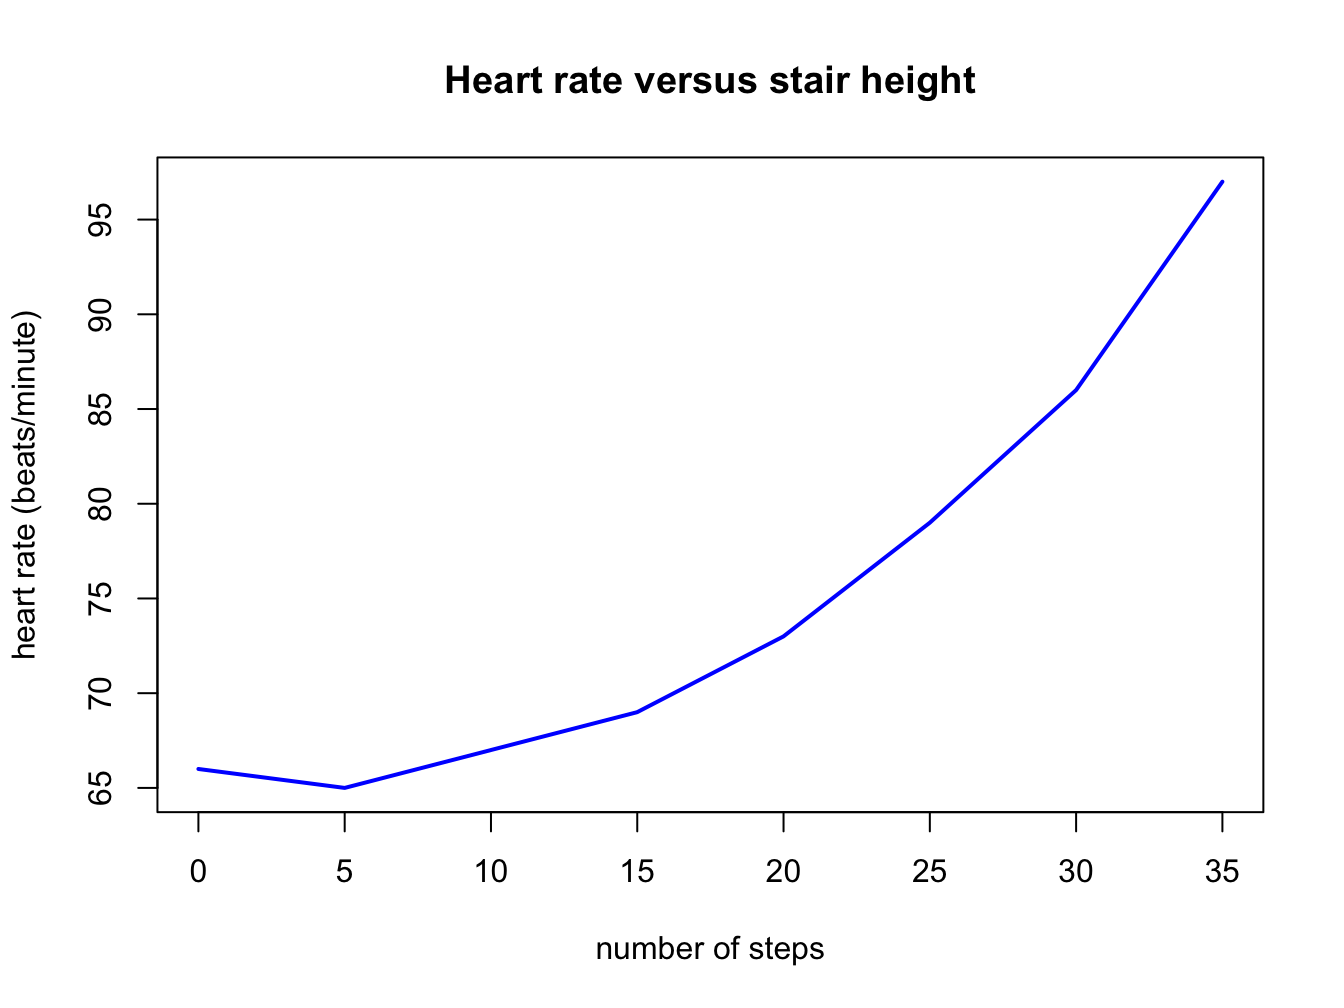
\includegraphics[width=0.8\linewidth]{davur_ebook_files/figure-latex/stair-walking-exp-1-1} \end{center}

\hypertarget{more-subjects-1}{%
\subsection{More subjects}\label{more-subjects-1}}

\begin{Shaded}
\begin{Highlighting}[]
\CommentTok{#number of steps on the stairs}
\NormalTok{stair_height <-}\StringTok{ }\KeywordTok{c}\NormalTok{(}\DecValTok{0}\NormalTok{, }\DecValTok{5}\NormalTok{, }\DecValTok{10}\NormalTok{, }\DecValTok{15}\NormalTok{, }\DecValTok{20}\NormalTok{, }\DecValTok{25}\NormalTok{, }\DecValTok{30}\NormalTok{, }\DecValTok{35}\NormalTok{)}
\CommentTok{#heart rates for subjects with normal weight}
\NormalTok{heart_rate_}\DecValTok{1}\NormalTok{ <-}\StringTok{ }\KeywordTok{c}\NormalTok{(}\DecValTok{66}\NormalTok{, }\DecValTok{65}\NormalTok{, }\DecValTok{67}\NormalTok{, }\DecValTok{69}\NormalTok{, }\DecValTok{73}\NormalTok{, }\DecValTok{79}\NormalTok{, }\DecValTok{86}\NormalTok{, }\DecValTok{97}\NormalTok{)}
\NormalTok{heart_rate_}\DecValTok{2}\NormalTok{ <-}\StringTok{ }\KeywordTok{c}\NormalTok{(}\DecValTok{61}\NormalTok{, }\DecValTok{61}\NormalTok{, }\DecValTok{63}\NormalTok{, }\DecValTok{68}\NormalTok{, }\DecValTok{74}\NormalTok{, }\DecValTok{81}\NormalTok{, }\DecValTok{89}\NormalTok{, }\DecValTok{104}\NormalTok{)}
\CommentTok{#heart rates for obese subjects}
\NormalTok{heart_rate_}\DecValTok{3}\NormalTok{ <-}\StringTok{ }\KeywordTok{c}\NormalTok{(}\DecValTok{58}\NormalTok{, }\DecValTok{60}\NormalTok{, }\DecValTok{67}\NormalTok{, }\DecValTok{71}\NormalTok{, }\DecValTok{78}\NormalTok{, }\DecValTok{89}\NormalTok{, }\DecValTok{104}\NormalTok{, }\DecValTok{121}\NormalTok{)}
\NormalTok{heart_rate_}\DecValTok{4}\NormalTok{ <-}\StringTok{ }\KeywordTok{c}\NormalTok{(}\DecValTok{69}\NormalTok{, }\DecValTok{73}\NormalTok{, }\DecValTok{77}\NormalTok{, }\DecValTok{83}\NormalTok{, }\DecValTok{88}\NormalTok{, }\DecValTok{96}\NormalTok{, }\DecValTok{102}\NormalTok{, }\DecValTok{127}\NormalTok{)}
\KeywordTok{plot}\NormalTok{(}\DataTypeTok{x =}\NormalTok{ stair_height,}
    \DataTypeTok{y =}\NormalTok{ heart_rate_}\DecValTok{1}\NormalTok{,}
    \DataTypeTok{main =} \StringTok{"Heart rate vs stair height"}\NormalTok{,}
    \DataTypeTok{xlab =} \StringTok{"number of steps"}\NormalTok{,}
    \DataTypeTok{ylab =} \StringTok{"heart rate (beats/min.)"}\NormalTok{,}
    \DataTypeTok{type =} \StringTok{"b"}\NormalTok{,}
    \DataTypeTok{lwd =} \DecValTok{2}\NormalTok{,}
    \DataTypeTok{col =} \StringTok{"green"}\NormalTok{,}
    \DataTypeTok{ylim =} \KeywordTok{c}\NormalTok{(}\DecValTok{55}\NormalTok{, }\DecValTok{130}\NormalTok{))}
\KeywordTok{points}\NormalTok{(}\DataTypeTok{x =}\NormalTok{ stair_height,}
    \DataTypeTok{y =}\NormalTok{ heart_rate_}\DecValTok{2}\NormalTok{,}
    \DataTypeTok{col =} \StringTok{"green"}\NormalTok{,}
    \DataTypeTok{type =} \StringTok{"b"}\NormalTok{,}
    \DataTypeTok{lwd =} \DecValTok{2}\NormalTok{)}
\KeywordTok{points}\NormalTok{(}\DataTypeTok{x =}\NormalTok{ stair_height,}
    \DataTypeTok{y =}\NormalTok{ heart_rate_}\DecValTok{3}\NormalTok{,}
    \DataTypeTok{col =} \StringTok{"red"}\NormalTok{,}
    \DataTypeTok{type =} \StringTok{"b"}\NormalTok{,}
    \DataTypeTok{lwd =} \DecValTok{2}\NormalTok{)}
\KeywordTok{points}\NormalTok{(}\DataTypeTok{x =}\NormalTok{ stair_height,}
    \DataTypeTok{y =}\NormalTok{ heart_rate_}\DecValTok{4}\NormalTok{,}
    \DataTypeTok{col =} \StringTok{"red"}\NormalTok{,}
    \DataTypeTok{type =} \StringTok{"b"}\NormalTok{,}
    \DataTypeTok{lwd =} \DecValTok{2}\NormalTok{)}
\end{Highlighting}
\end{Shaded}

\begin{center}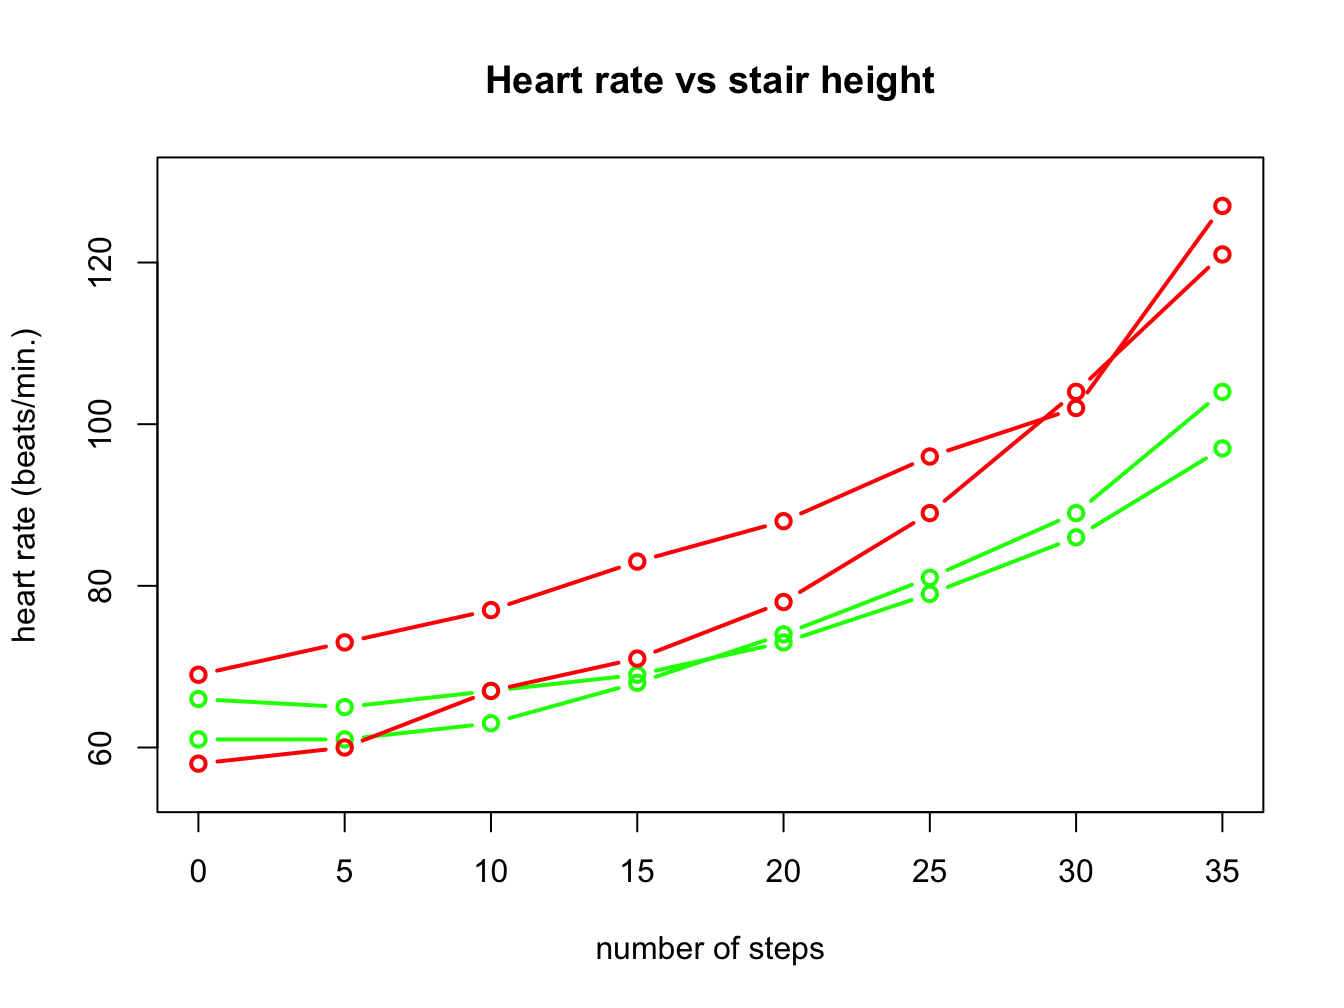
\includegraphics[width=0.8\linewidth]{davur_ebook_files/figure-latex/stair-walking-exp-2-1} \end{center}

\hypertarget{chickens-on-a-diet-1}{%
\subsection{Chickens on a diet}\label{chickens-on-a-diet-1}}

\begin{Shaded}
\begin{Highlighting}[]
\NormalTok{time <-}\StringTok{ }\KeywordTok{c}\NormalTok{(}\DecValTok{0}\NormalTok{, }\DecValTok{2}\NormalTok{, }\DecValTok{4}\NormalTok{, }\DecValTok{6}\NormalTok{, }\DecValTok{8}\NormalTok{, }\DecValTok{10}\NormalTok{, }\DecValTok{12}\NormalTok{, }\DecValTok{14}\NormalTok{, }\DecValTok{16}\NormalTok{, }\DecValTok{18}\NormalTok{, }\DecValTok{20}\NormalTok{, }\DecValTok{21}\NormalTok{)}
\NormalTok{chick_}\DecValTok{1}\NormalTok{ <-}\StringTok{ }\KeywordTok{c}\NormalTok{(}\DecValTok{42}\NormalTok{, }\DecValTok{51}\NormalTok{, }\DecValTok{59}\NormalTok{, }\DecValTok{64}\NormalTok{, }\DecValTok{76}\NormalTok{, }\DecValTok{93}\NormalTok{, }\DecValTok{106}\NormalTok{, }\DecValTok{125}\NormalTok{, }\DecValTok{149}\NormalTok{, }\DecValTok{171}\NormalTok{, }\DecValTok{199}\NormalTok{, }\DecValTok{205}\NormalTok{)}
\NormalTok{chick_}\DecValTok{2}\NormalTok{ <-}\StringTok{ }\KeywordTok{c}\NormalTok{(}\DecValTok{40}\NormalTok{, }\DecValTok{49}\NormalTok{, }\DecValTok{58}\NormalTok{, }\DecValTok{72}\NormalTok{, }\DecValTok{84}\NormalTok{, }\DecValTok{103}\NormalTok{, }\DecValTok{122}\NormalTok{, }\DecValTok{138}\NormalTok{, }\DecValTok{162}\NormalTok{, }\DecValTok{187}\NormalTok{, }\DecValTok{209}\NormalTok{, }\DecValTok{215}\NormalTok{)}
\NormalTok{chick_}\DecValTok{3}\NormalTok{ <-}\StringTok{ }\KeywordTok{c}\NormalTok{(}\DecValTok{42}\NormalTok{, }\DecValTok{53}\NormalTok{, }\DecValTok{62}\NormalTok{, }\DecValTok{73}\NormalTok{, }\DecValTok{85}\NormalTok{, }\DecValTok{102}\NormalTok{, }\DecValTok{123}\NormalTok{, }\DecValTok{138}\NormalTok{, }\DecValTok{170}\NormalTok{, }\DecValTok{204}\NormalTok{, }\DecValTok{235}\NormalTok{, }\DecValTok{256}\NormalTok{)}
\NormalTok{chick_}\DecValTok{4}\NormalTok{ <-}\StringTok{ }\KeywordTok{c}\NormalTok{(}\DecValTok{41}\NormalTok{, }\DecValTok{49}\NormalTok{, }\DecValTok{61}\NormalTok{, }\DecValTok{74}\NormalTok{, }\DecValTok{98}\NormalTok{, }\DecValTok{109}\NormalTok{, }\DecValTok{128}\NormalTok{, }\DecValTok{154}\NormalTok{, }\DecValTok{192}\NormalTok{, }\DecValTok{232}\NormalTok{, }\DecValTok{280}\NormalTok{, }\DecValTok{290}\NormalTok{)}

\KeywordTok{plot}\NormalTok{(}\DataTypeTok{x =}\NormalTok{ time, }\DataTypeTok{y =}\NormalTok{ chick_}\DecValTok{1}\NormalTok{,}
         \DataTypeTok{type =} \StringTok{"l"}\NormalTok{,}
         \DataTypeTok{lwd =} \DecValTok{2}\NormalTok{,}
         \DataTypeTok{col =} \StringTok{"blue"}\NormalTok{,}
         \DataTypeTok{ylim =} \KeywordTok{c}\NormalTok{(}\DecValTok{40}\NormalTok{, }\DecValTok{300}\NormalTok{))}
\KeywordTok{points}\NormalTok{(}\DataTypeTok{x =}\NormalTok{ time, }\DataTypeTok{y =}\NormalTok{ chick_}\DecValTok{2}\NormalTok{,}
         \DataTypeTok{type =} \StringTok{"l"}\NormalTok{,}
         \DataTypeTok{lwd =} \DecValTok{2}\NormalTok{,}
         \DataTypeTok{lty =} \DecValTok{3}\NormalTok{,}
         \DataTypeTok{col =} \StringTok{"blue"}\NormalTok{)}
\KeywordTok{points}\NormalTok{(}\DataTypeTok{x =}\NormalTok{ time, }\DataTypeTok{y =}\NormalTok{ chick_}\DecValTok{3}\NormalTok{,}
         \DataTypeTok{type =} \StringTok{"l"}\NormalTok{,}
         \DataTypeTok{lwd =} \DecValTok{2}\NormalTok{,}
         \DataTypeTok{lty =} \DecValTok{1}\NormalTok{,}
         \DataTypeTok{col =} \StringTok{"red"}\NormalTok{)}
\KeywordTok{points}\NormalTok{(}\DataTypeTok{x =}\NormalTok{ time, }\DataTypeTok{y =}\NormalTok{ chick_}\DecValTok{4}\NormalTok{,}
         \DataTypeTok{type =} \StringTok{"l"}\NormalTok{,}
         \DataTypeTok{lwd =} \DecValTok{2}\NormalTok{,}
         \DataTypeTok{lty =} \DecValTok{3}\NormalTok{,}
         \DataTypeTok{col =} \StringTok{"red"}\NormalTok{)}
\end{Highlighting}
\end{Shaded}

\begin{center}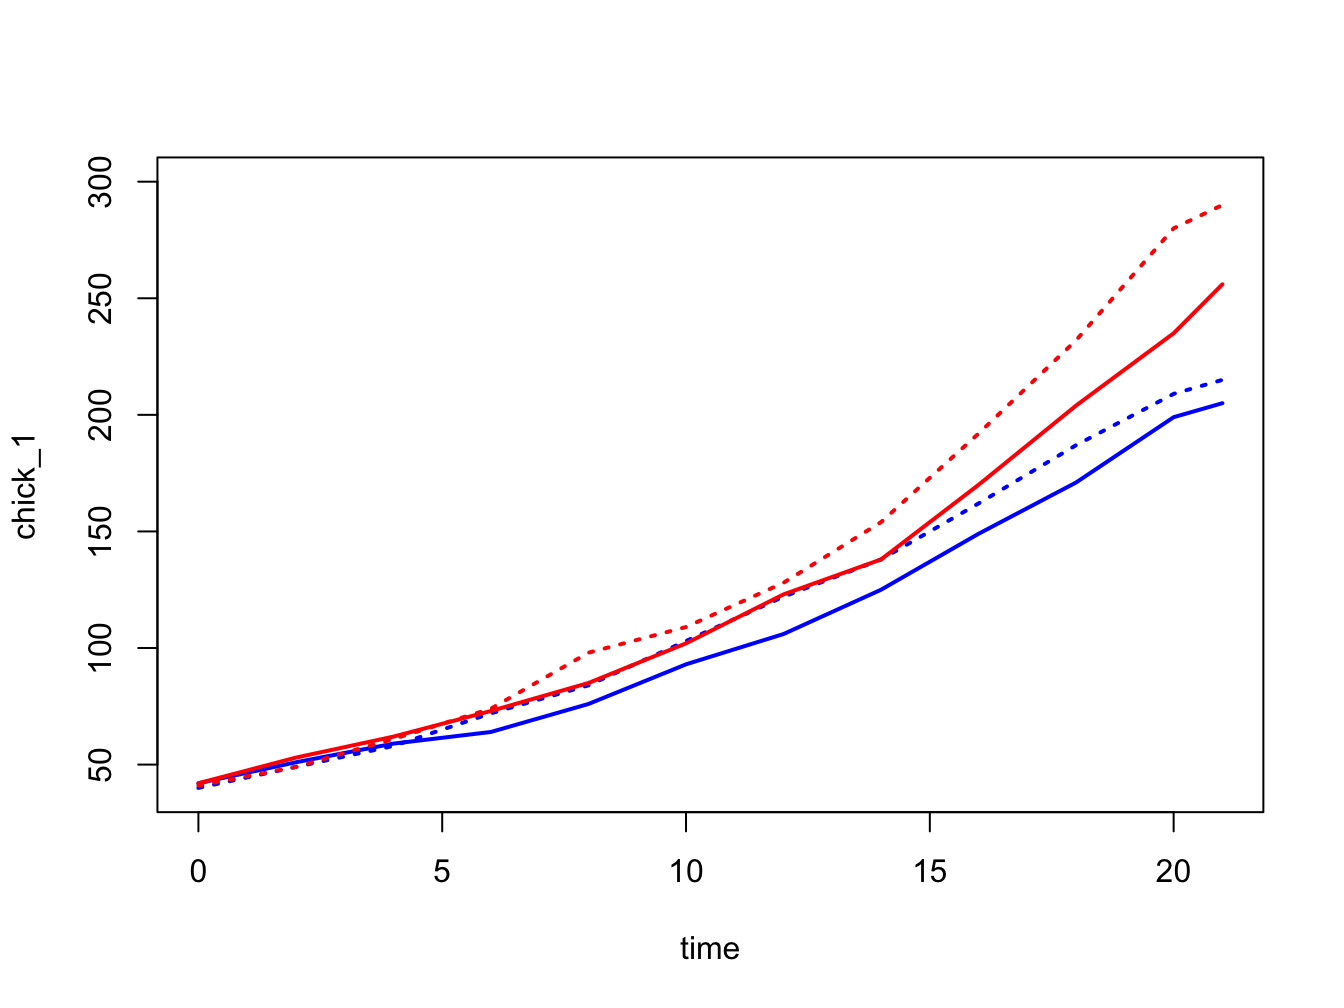
\includegraphics[width=0.8\linewidth]{davur_ebook_files/figure-latex/chicken-diets1-1} \end{center}

\hypertarget{chicken-bar-plot-1}{%
\subsection{Chicken bar plot}\label{chicken-bar-plot-1}}

\begin{Shaded}
\begin{Highlighting}[]
\NormalTok{maxima <-}\StringTok{ }\KeywordTok{c}\NormalTok{(}\KeywordTok{max}\NormalTok{(chick_}\DecValTok{1}\NormalTok{), }\KeywordTok{max}\NormalTok{(chick_}\DecValTok{2}\NormalTok{), }\KeywordTok{max}\NormalTok{(chick_}\DecValTok{3}\NormalTok{), }\KeywordTok{max}\NormalTok{(chick_}\DecValTok{4}\NormalTok{))}

\KeywordTok{barplot}\NormalTok{(maxima,}
    \DataTypeTok{names =} \KeywordTok{c}\NormalTok{(}\StringTok{"Chick 1"}\NormalTok{,}\StringTok{"Chick 2"}\NormalTok{,}\StringTok{"Chick 3"}\NormalTok{,}\StringTok{"Chick 4"}\NormalTok{),}
    \DataTypeTok{ylab =} \StringTok{"Maximum weight (grams)"}\NormalTok{,}
    \DataTypeTok{col =} \StringTok{"gold"}\NormalTok{,}
    \DataTypeTok{main =} \StringTok{"Maximum chick weights"}\NormalTok{)}
\end{Highlighting}
\end{Shaded}

\begin{center}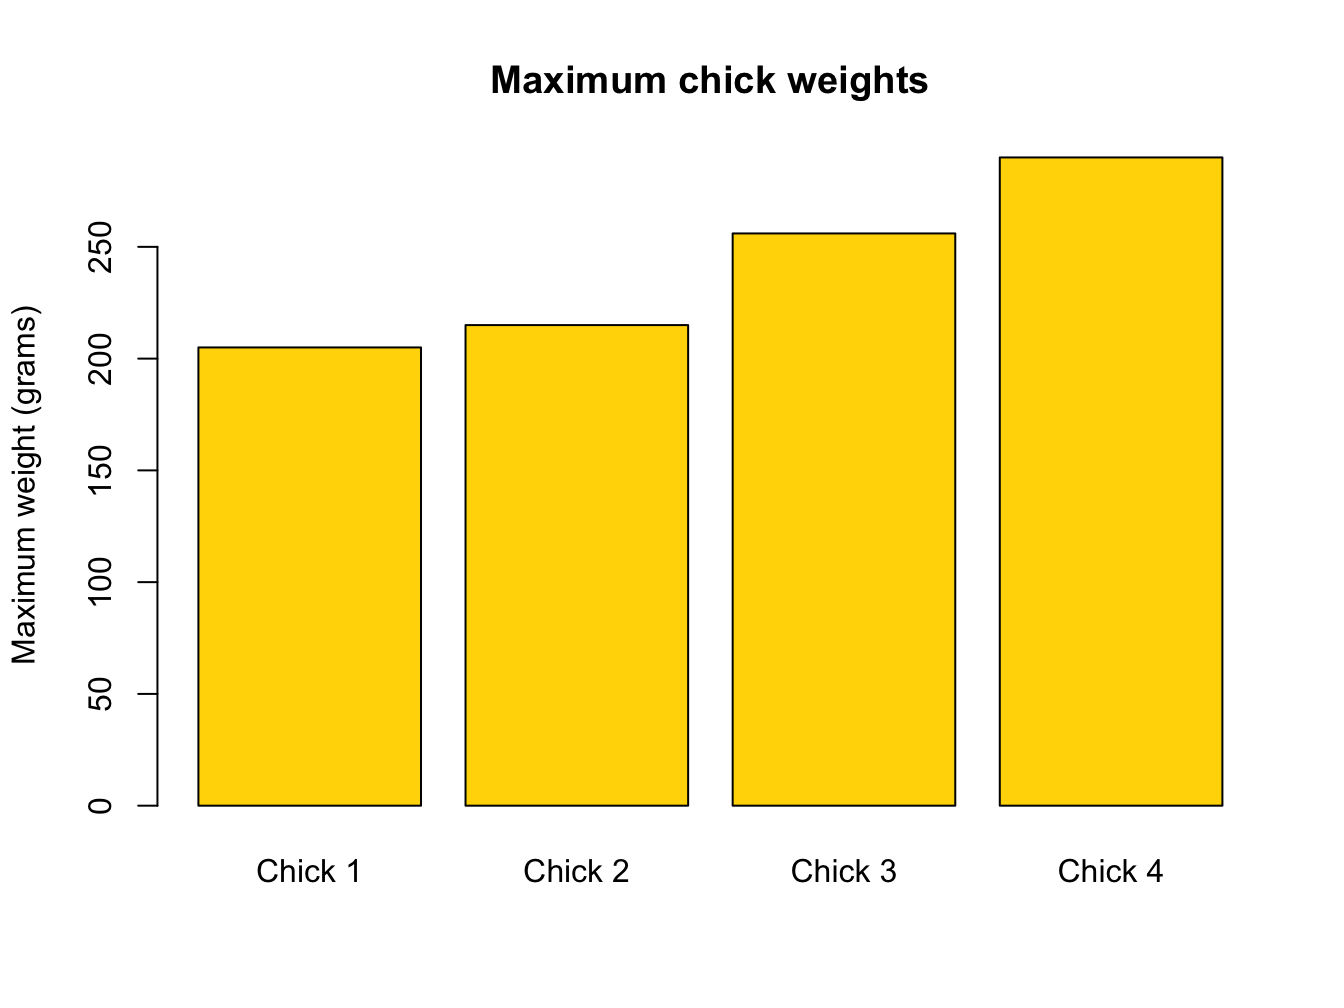
\includegraphics[width=0.8\linewidth]{davur_ebook_files/figure-latex/chicken-diets2-1} \end{center}

\hypertarget{discoveries-1}{%
\subsection{Discoveries}\label{discoveries-1}}

\textbf{A}

\begin{Shaded}
\begin{Highlighting}[]
\KeywordTok{barplot}\NormalTok{(}\KeywordTok{table}\NormalTok{(discoveries),}
    \DataTypeTok{main =} \StringTok{"great discoveries per year"}\NormalTok{,}
    \DataTypeTok{xlab =} \StringTok{"number of discoveries"}\NormalTok{,}
    \DataTypeTok{ylab =} \StringTok{"frequency"}\NormalTok{,}
    \DataTypeTok{col =} \StringTok{"green"}\NormalTok{)}
\end{Highlighting}
\end{Shaded}

\begin{center}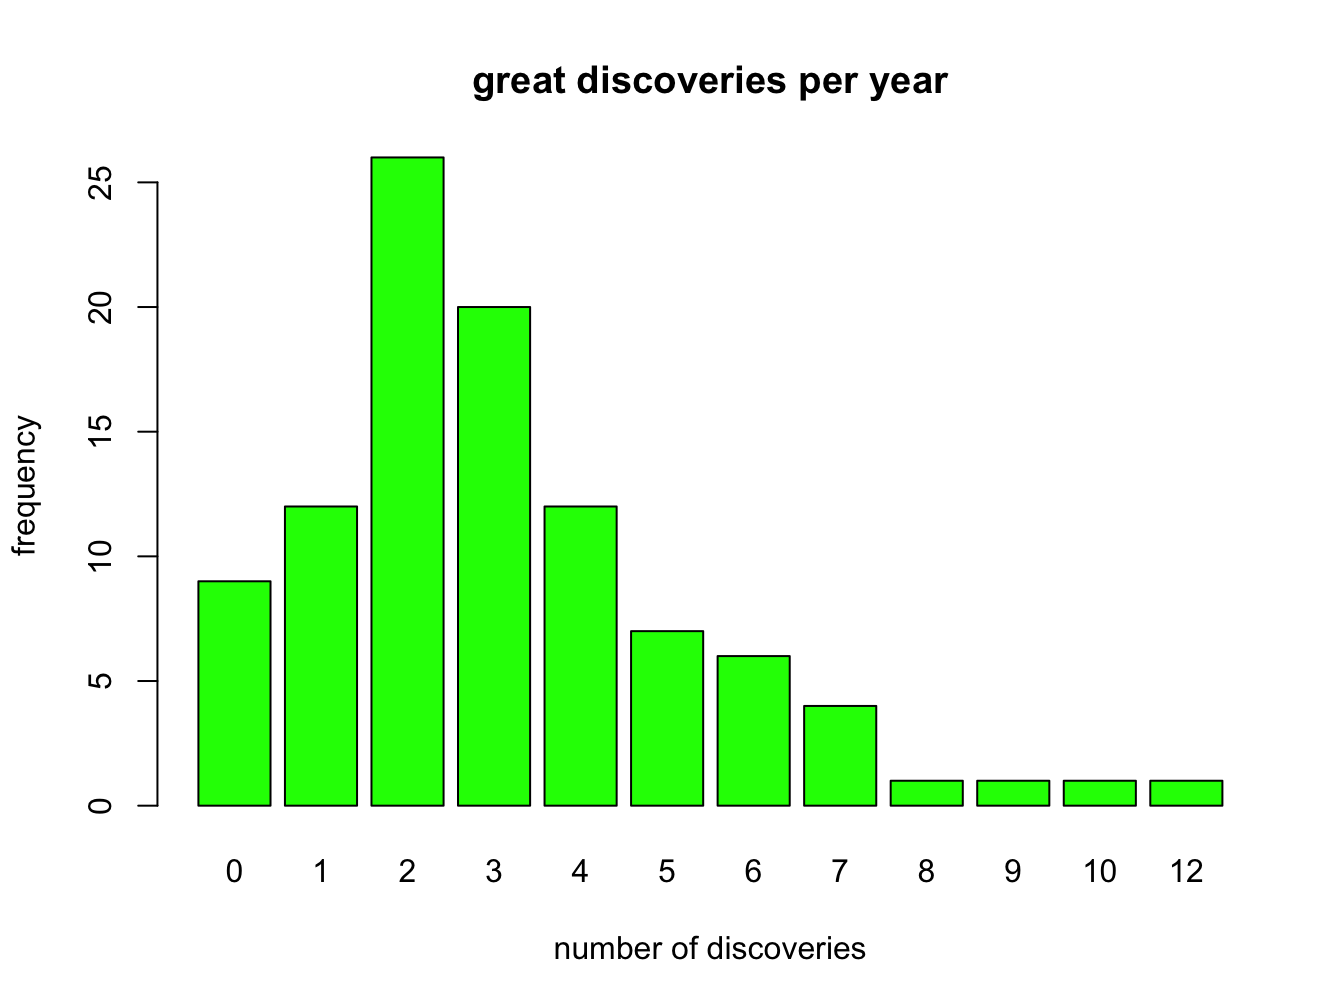
\includegraphics[width=0.8\linewidth]{davur_ebook_files/figure-latex/discoveries-1-1} \end{center}

\textbf{B}

\begin{Shaded}
\begin{Highlighting}[]
\KeywordTok{summary}\NormalTok{(discoveries)}
\end{Highlighting}
\end{Shaded}

\textbf{C}

\begin{Shaded}
\begin{Highlighting}[]
\KeywordTok{plot}\NormalTok{(discoveries,}
         \DataTypeTok{xlab =} \StringTok{"year"}\NormalTok{,}
         \DataTypeTok{ylab =} \StringTok{"number of discoveries"}\NormalTok{,}
         \DataTypeTok{main =} \StringTok{"Great discoveries"}\NormalTok{,}
         \DataTypeTok{col =} \StringTok{"blue"}\NormalTok{, }
         \DataTypeTok{lwd =} \DecValTok{2}\NormalTok{)}
\end{Highlighting}
\end{Shaded}

\begin{center}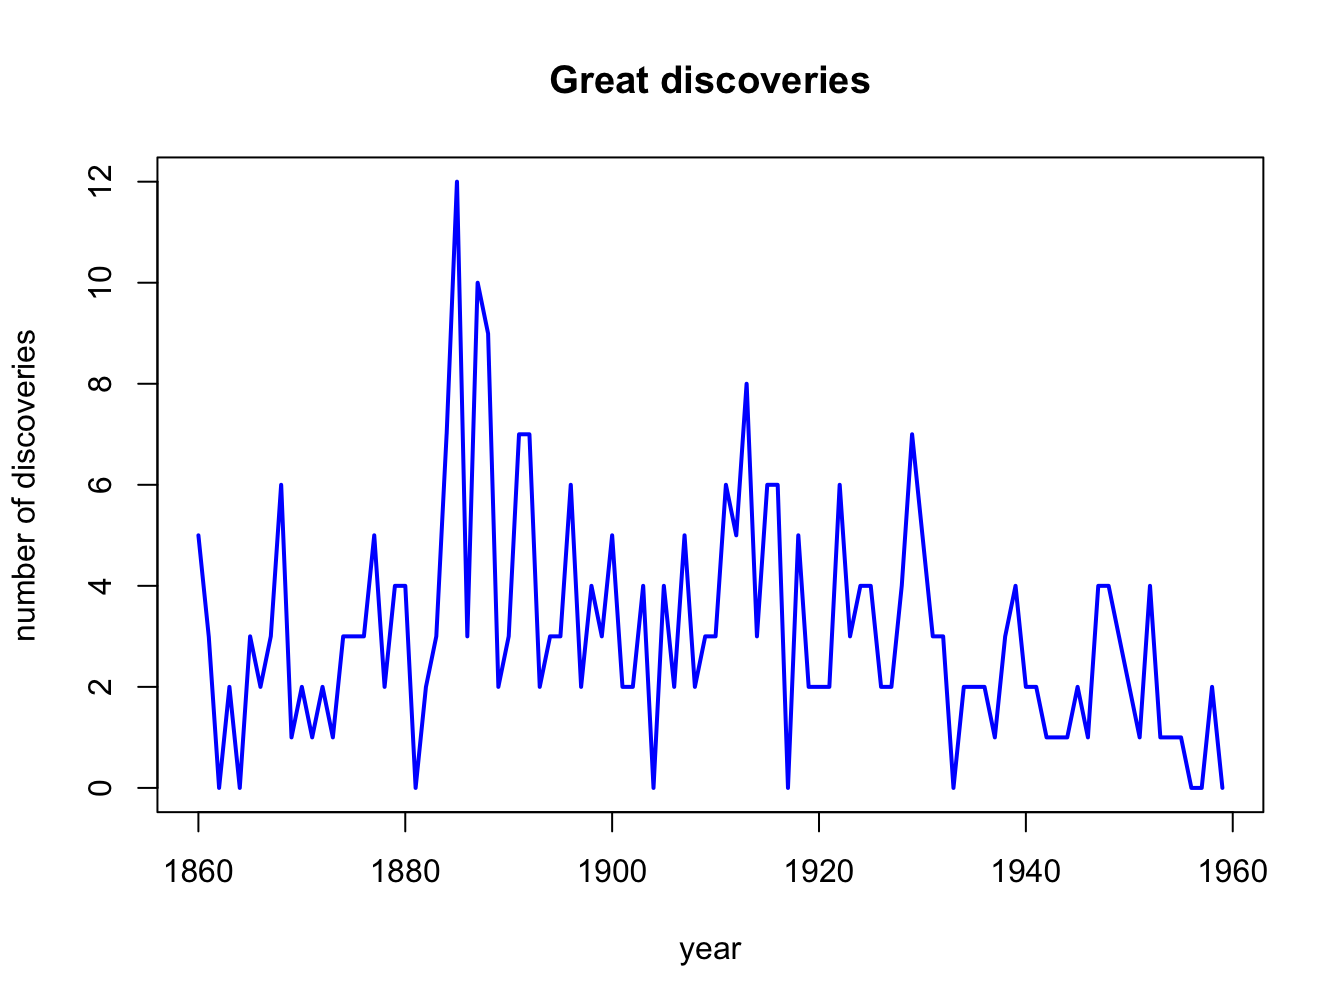
\includegraphics[width=0.8\linewidth]{davur_ebook_files/figure-latex/discoveries-3-1} \end{center}

\hypertarget{lung-cancer-1}{%
\subsection{Lung cancer}\label{lung-cancer-1}}

\textbf{A}

\begin{Shaded}
\begin{Highlighting}[]
\NormalTok{total.col <-}\StringTok{ "red"}
\NormalTok{m.col <-}\StringTok{ "blue"}
\NormalTok{f.col <-}\StringTok{ "green"}
\KeywordTok{plot}\NormalTok{(ldeaths,}
         \DataTypeTok{main =} \StringTok{"deaths from lung cancer"}\NormalTok{,}
         \DataTypeTok{xlab =} \StringTok{"year"}\NormalTok{,}
         \DataTypeTok{ylab =} \StringTok{"number"}\NormalTok{,}
         \DataTypeTok{col =}\NormalTok{ total.col,}
         \DataTypeTok{ylim =} \KeywordTok{c}\NormalTok{(}\DecValTok{0}\NormalTok{, }\DecValTok{4000}\NormalTok{),}
         \DataTypeTok{lwd =} \DecValTok{2}
\NormalTok{)}
\KeywordTok{lines}\NormalTok{(fdeaths, }\DataTypeTok{col =}\NormalTok{ f.col, }\DataTypeTok{lwd =} \DecValTok{2}\NormalTok{)}
\KeywordTok{lines}\NormalTok{(mdeaths, }\DataTypeTok{col =}\NormalTok{ m.col, }\DataTypeTok{lwd =} \DecValTok{2}\NormalTok{)}
\KeywordTok{legend}\NormalTok{(}
    \StringTok{"topleft"}\NormalTok{, }
    \DataTypeTok{legend =} \KeywordTok{c}\NormalTok{(}\StringTok{"total"}\NormalTok{, }\StringTok{"female"}\NormalTok{, }\StringTok{"male"}\NormalTok{), }
    \DataTypeTok{col =} \KeywordTok{c}\NormalTok{(total.col, f.col, m.col), }
    \DataTypeTok{lty =} \DecValTok{1}\NormalTok{)}
\end{Highlighting}
\end{Shaded}

\begin{center}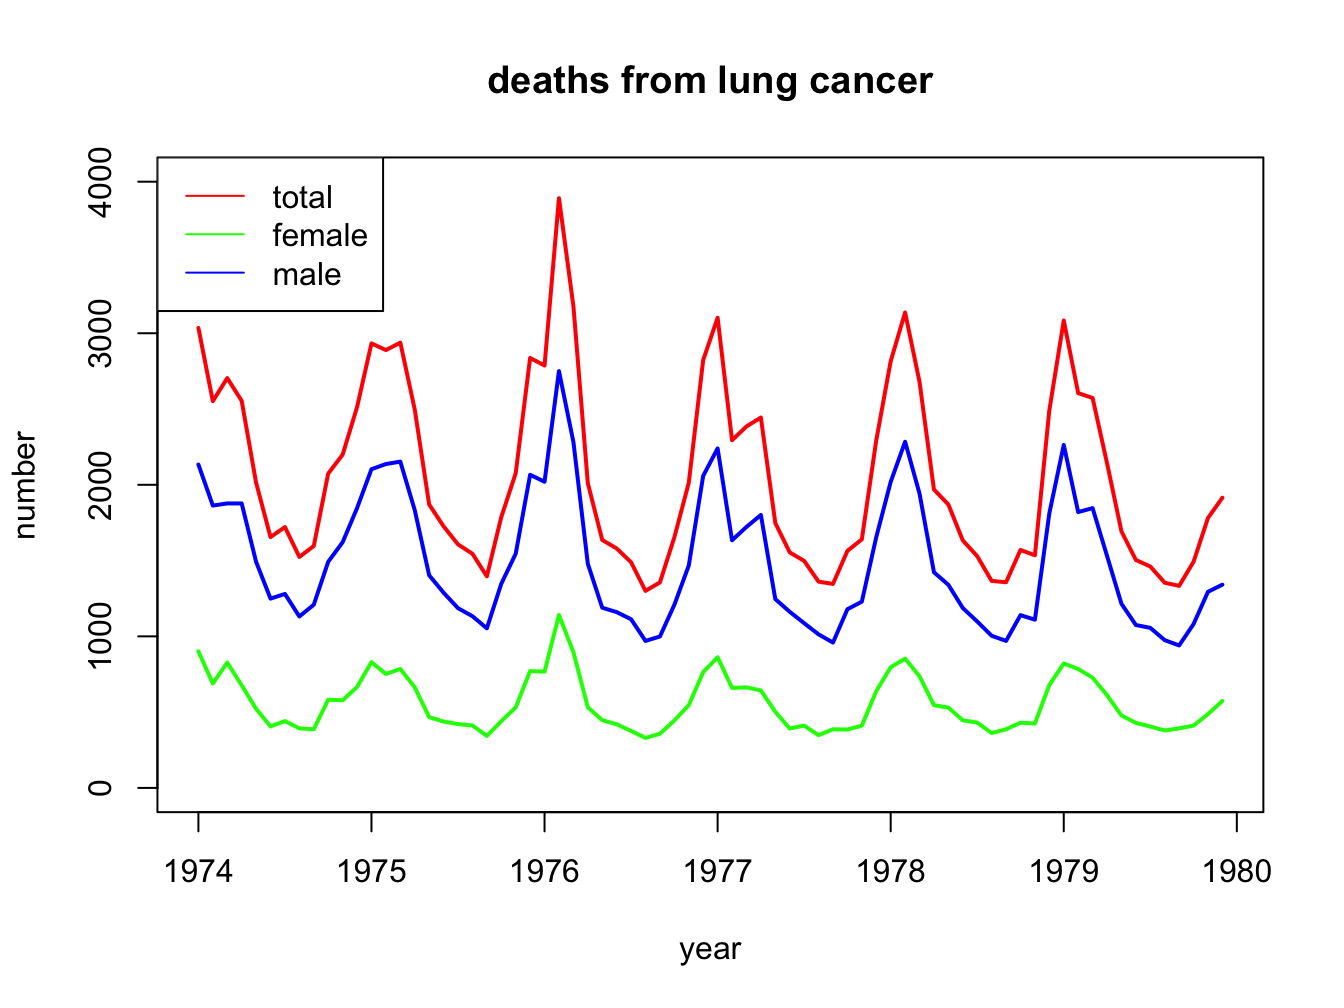
\includegraphics[width=0.8\linewidth]{davur_ebook_files/figure-latex/lung-cancer-1-1} \end{center}

\textbf{B}

Create a combined boxplot of the three time-series. Are they indicative of a normal distribution? Are there outliers? If so, can you figure out when this occurred?

\begin{Shaded}
\begin{Highlighting}[]
\KeywordTok{boxplot}\NormalTok{(}
\NormalTok{    fdeaths, mdeaths, ldeaths}
\NormalTok{)}
\end{Highlighting}
\end{Shaded}

\begin{center}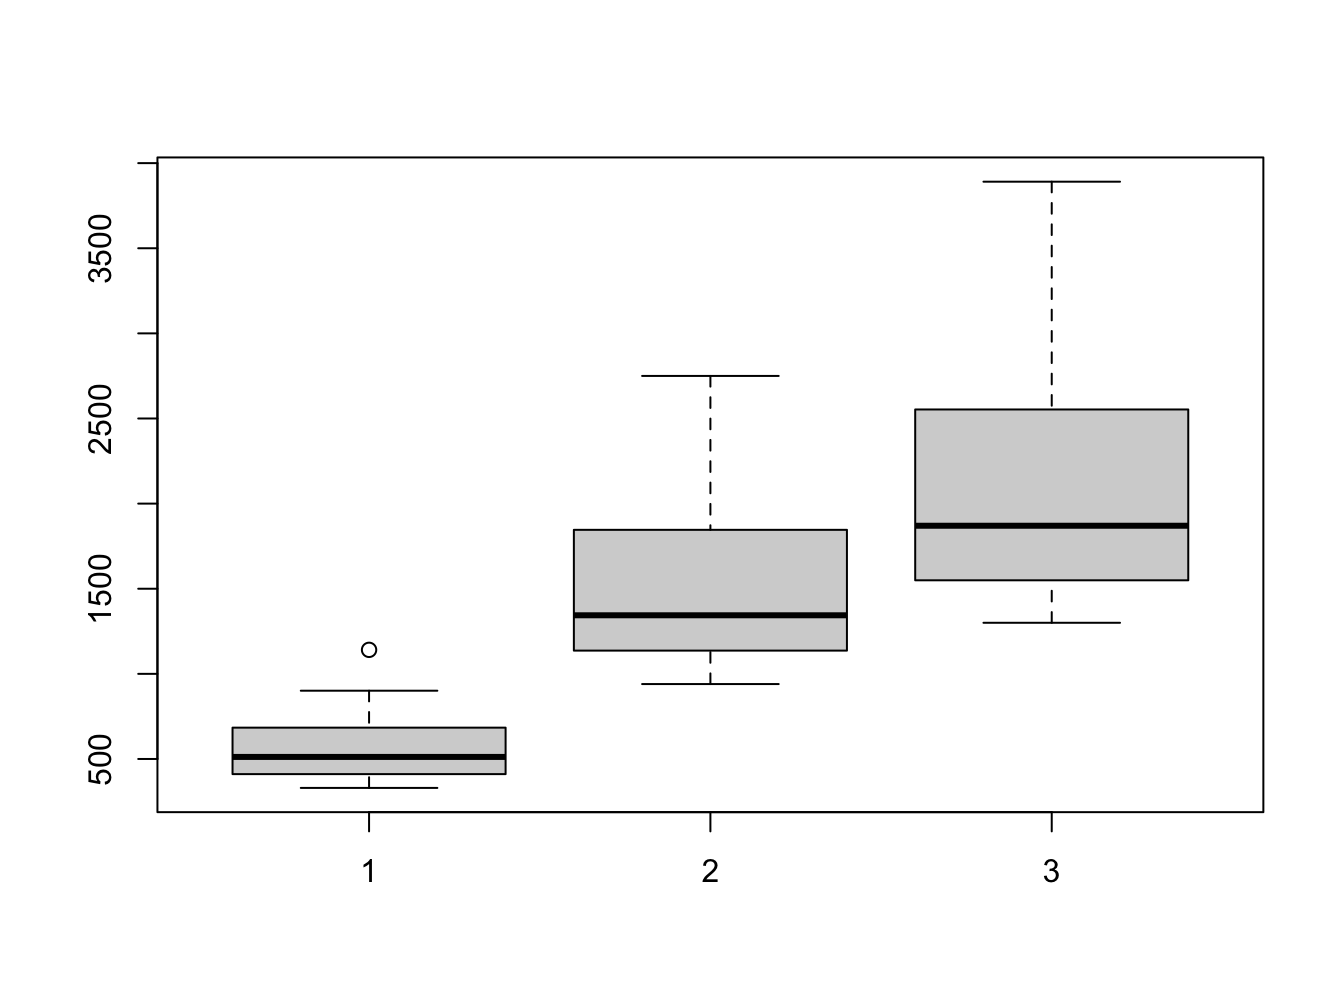
\includegraphics[width=0.8\linewidth]{davur_ebook_files/figure-latex/lung-cancer-2-1} \end{center}

\hypertarget{complex-datatypes-2}{%
\section{Complex datatypes}\label{complex-datatypes-2}}

\hypertarget{creating-factors-1}{%
\subsection{Creating factors}\label{creating-factors-1}}

\textbf{A}

\begin{Shaded}
\begin{Highlighting}[]
\NormalTok{animal_risk <-}\StringTok{ }\KeywordTok{c}\NormalTok{(}\DecValTok{2}\NormalTok{, }\DecValTok{4}\NormalTok{, }\DecValTok{1}\NormalTok{, }\DecValTok{1}\NormalTok{, }\DecValTok{2}\NormalTok{, }\DecValTok{4}\NormalTok{, }\DecValTok{1}\NormalTok{, }\DecValTok{4}\NormalTok{, }\DecValTok{1}\NormalTok{, }\DecValTok{1}\NormalTok{, }\DecValTok{2}\NormalTok{, }\DecValTok{1}\NormalTok{)}
\NormalTok{animal_risk_factor <-}\StringTok{ }\KeywordTok{factor}\NormalTok{(}\DataTypeTok{x =}\NormalTok{ animal_risk,}
                             \DataTypeTok{levels =} \KeywordTok{c}\NormalTok{(}\DecValTok{1}\NormalTok{, }\DecValTok{2}\NormalTok{, }\DecValTok{3}\NormalTok{, }\DecValTok{4}\NormalTok{),}
                             \DataTypeTok{labels =} \KeywordTok{c}\NormalTok{(}\StringTok{"harmless"}\NormalTok{, }\StringTok{"risky"}\NormalTok{, }\StringTok{"dangerous"}\NormalTok{, }\StringTok{"deadly"}\NormalTok{),}
                             \DataTypeTok{ordered =} \OtherTok{TRUE}\NormalTok{)}
\KeywordTok{barplot}\NormalTok{(}\KeywordTok{table}\NormalTok{(animal_risk_factor))}
\end{Highlighting}
\end{Shaded}

\textbf{B}

\begin{Shaded}
\begin{Highlighting}[]
\KeywordTok{set.seed}\NormalTok{(}\DecValTok{1234}\NormalTok{)}
\NormalTok{wealth_male <-}\StringTok{ }\KeywordTok{sample}\NormalTok{(}\DataTypeTok{x =}\NormalTok{ letters[}\DecValTok{1}\OperatorTok{:}\DecValTok{4}\NormalTok{], }
                 \DataTypeTok{size =} \DecValTok{1000}\NormalTok{,}
                 \DataTypeTok{replace=} \OtherTok{TRUE}\NormalTok{, }
                 \DataTypeTok{prob =} \KeywordTok{c}\NormalTok{(}\FloatTok{0.7}\NormalTok{, }\FloatTok{0.17}\NormalTok{, }\FloatTok{0.12}\NormalTok{, }\FloatTok{0.01}\NormalTok{))}
\NormalTok{wealth_female <-}\StringTok{ }\KeywordTok{sample}\NormalTok{(}\DataTypeTok{x =}\NormalTok{ letters[}\DecValTok{1}\OperatorTok{:}\DecValTok{4}\NormalTok{], }
                 \DataTypeTok{size =} \DecValTok{1000}\NormalTok{,}
                 \DataTypeTok{replace=} \OtherTok{TRUE}\NormalTok{, }
                 \DataTypeTok{prob =} \KeywordTok{c}\NormalTok{(}\FloatTok{0.8}\NormalTok{, }\FloatTok{0.15}\NormalTok{, }\FloatTok{0.497}\NormalTok{, }\FloatTok{0.003}\NormalTok{))}

\NormalTok{wealth_labels <-}\StringTok{ }\KeywordTok{c}\NormalTok{(}\StringTok{"poor"}\NormalTok{, }\StringTok{"middle class"}\NormalTok{, }\StringTok{"wealthy"}\NormalTok{, }\StringTok{"rich"}\NormalTok{)}

\NormalTok{wealth_male_f <-}\StringTok{ }\KeywordTok{factor}\NormalTok{(}\DataTypeTok{x =}\NormalTok{ wealth_male,}
                        \DataTypeTok{levels =}\NormalTok{ letters[}\DecValTok{1}\OperatorTok{:}\DecValTok{4}\NormalTok{],}
                        \DataTypeTok{labels =}\NormalTok{ wealth_labels,}
                        \DataTypeTok{ordered =} \OtherTok{TRUE}\NormalTok{)}

\NormalTok{wealth_female_f <-}\StringTok{ }\KeywordTok{factor}\NormalTok{(}\DataTypeTok{x =}\NormalTok{ wealth_female,}
                        \DataTypeTok{levels =}\NormalTok{ letters[}\DecValTok{1}\OperatorTok{:}\DecValTok{4}\NormalTok{],}
                        \DataTypeTok{labels =}\NormalTok{ wealth_labels,}
                        \DataTypeTok{ordered =} \OtherTok{TRUE}\NormalTok{)}

\CommentTok{#combine}
\NormalTok{wealth_all_f <-}\StringTok{ }\KeywordTok{factor}\NormalTok{(}\KeywordTok{c}\NormalTok{(wealth_male_f, wealth_female_f),}
                        \DataTypeTok{levels =} \DecValTok{1}\OperatorTok{:}\DecValTok{4}\NormalTok{,}
                        \DataTypeTok{labels =}\NormalTok{ wealth_labels,}
                        \DataTypeTok{ordered =} \OtherTok{TRUE}\NormalTok{)}

\KeywordTok{prop.table}\NormalTok{(}\KeywordTok{table}\NormalTok{(wealth_all_f)) }\OperatorTok{*}\StringTok{ }\DecValTok{100}
\end{Highlighting}
\end{Shaded}

\begin{verbatim}
## wealth_all_f
##         poor middle class      wealthy         rich 
##        63.65        12.45        23.35         0.55
\end{verbatim}

\begin{Shaded}
\begin{Highlighting}[]
\CommentTok{#getting this data right may be a bit of a challenge...}
\NormalTok{bar_data <-}\StringTok{ }\KeywordTok{rbind}\NormalTok{(}\KeywordTok{table}\NormalTok{(wealth_female_f), }\KeywordTok{table}\NormalTok{(wealth_male_f))}
\KeywordTok{rownames}\NormalTok{(bar_data) <-}\StringTok{ }\KeywordTok{c}\NormalTok{(}\StringTok{"female"}\NormalTok{, }\StringTok{"male"}\NormalTok{)}

\KeywordTok{barplot}\NormalTok{(bar_data, }\DataTypeTok{beside =}\NormalTok{ T, }\DataTypeTok{legend =} \KeywordTok{rownames}\NormalTok{(bar_data))}
\end{Highlighting}
\end{Shaded}

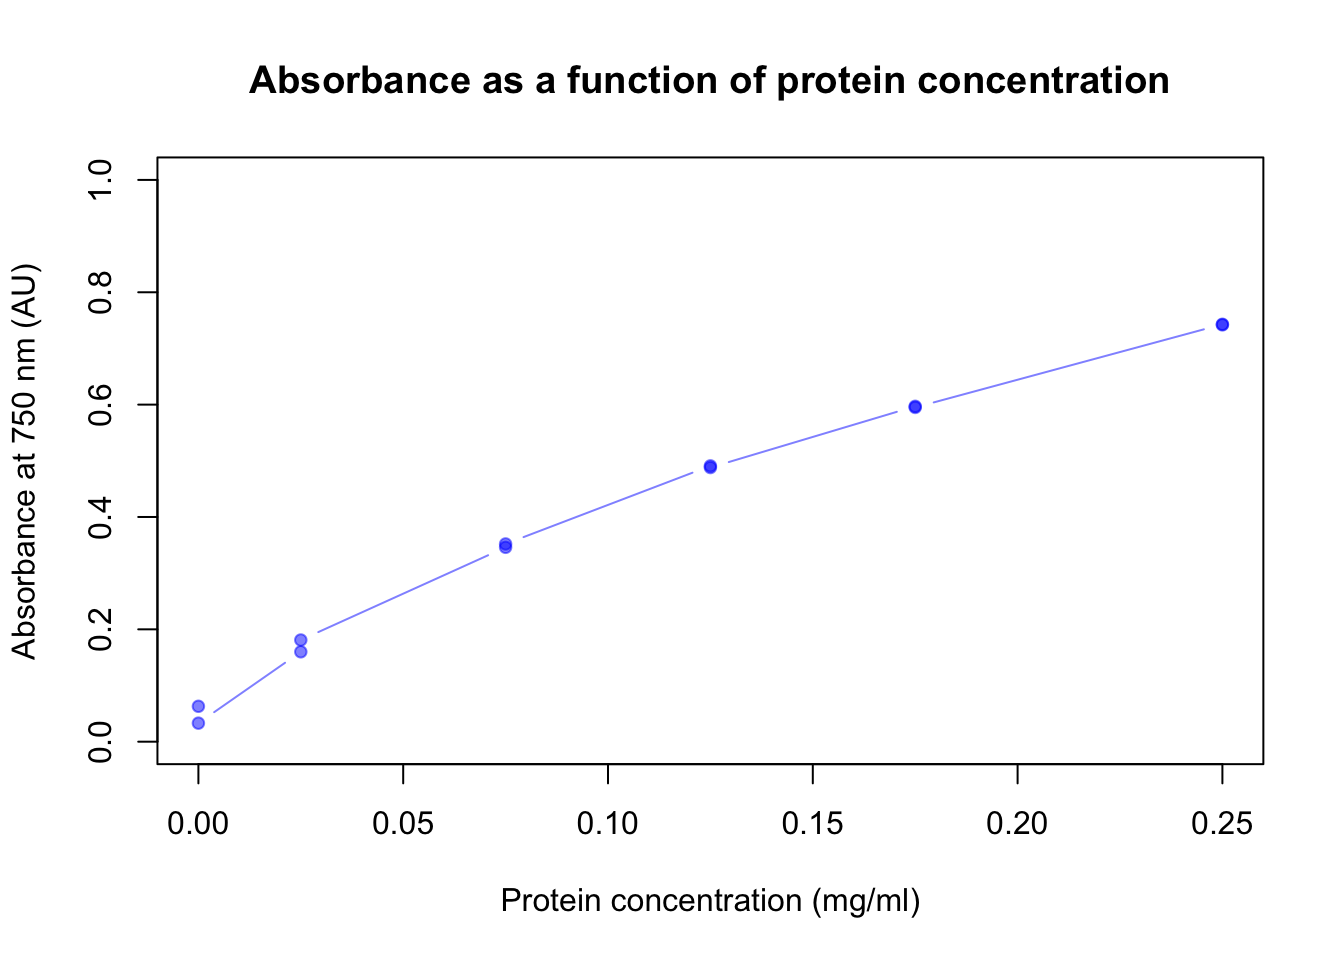
\includegraphics{davur_ebook_files/figure-latex/unnamed-chunk-13-1.pdf}

\hypertarget{a-dictionary-with-a-named-vector-1}{%
\subsection{A dictionary with a named vector}\label{a-dictionary-with-a-named-vector-1}}

\textbf{A}

\begin{Shaded}
\begin{Highlighting}[]
\NormalTok{codons <-}\StringTok{ }\KeywordTok{c}\NormalTok{(}\StringTok{"G"}\NormalTok{, }\StringTok{"P"}\NormalTok{, }\StringTok{"K"}\NormalTok{, }\StringTok{"S"}\NormalTok{)}
\KeywordTok{names}\NormalTok{(codons) <-}\StringTok{ }\KeywordTok{c}\NormalTok{(}\StringTok{"GGA"}\NormalTok{, }\StringTok{"CCU"}\NormalTok{, }\StringTok{"AAA"}\NormalTok{, }\StringTok{"AGU"}\NormalTok{)}

\NormalTok{my_DNA <-}\StringTok{ "GGACCUAAAAGU"}
\NormalTok{my_prot <-}\StringTok{ ""}
\ControlFlowTok{for}\NormalTok{ (i }\ControlFlowTok{in} \KeywordTok{seq}\NormalTok{(}\DataTypeTok{from =} \DecValTok{1}\NormalTok{, }\DataTypeTok{to =} \KeywordTok{nchar}\NormalTok{(my_DNA), }\DataTypeTok{by =} \DecValTok{3}\NormalTok{)) \{}
\NormalTok{        codon <-}\StringTok{ }\KeywordTok{substr}\NormalTok{(my_DNA, i, i}\OperatorTok{+}\DecValTok{2}\NormalTok{)}
\NormalTok{        my_prot <-}\StringTok{ }\KeywordTok{paste0}\NormalTok{(my_prot, codons[codon])}
\NormalTok{\}}
\KeywordTok{print}\NormalTok{(my_prot)}
\end{Highlighting}
\end{Shaded}

\begin{verbatim}
## [1] "GPKS"
\end{verbatim}

\textbf{B}

\begin{Shaded}
\begin{Highlighting}[]
\NormalTok{nuc_weights <-}\StringTok{ }\KeywordTok{c}\NormalTok{(}\FloatTok{491.2}\NormalTok{, }\FloatTok{467.2}\NormalTok{, }\FloatTok{507.2}\NormalTok{, }\FloatTok{482.2}\NormalTok{)}
\KeywordTok{names}\NormalTok{(nuc_weights) <-}\StringTok{ }\KeywordTok{c}\NormalTok{(}\StringTok{'A'}\NormalTok{, }\StringTok{'C'}\NormalTok{, }\StringTok{'G'}\NormalTok{, }\StringTok{'U'}\NormalTok{)}

\NormalTok{mol_weight <-}\StringTok{ }\DecValTok{0}
\ControlFlowTok{for}\NormalTok{ (i }\ControlFlowTok{in} \DecValTok{1}\OperatorTok{:}\KeywordTok{nchar}\NormalTok{(my_DNA)) \{}
\NormalTok{        nuc <-}\StringTok{ }\KeywordTok{substr}\NormalTok{(my_DNA, i, i);}
        \KeywordTok{print}\NormalTok{(nuc)}
\NormalTok{        mol_weight <-}\StringTok{ }\NormalTok{mol_weight }\OperatorTok{+}\StringTok{ }\NormalTok{nuc_weights[nuc]}
\NormalTok{\}}
\NormalTok{mol_weight}
\end{Highlighting}
\end{Shaded}

\hypertarget{airquality-1}{%
\subsection{airquality}\label{airquality-1}}

\textbf{A}

\begin{Shaded}
\begin{Highlighting}[]
\KeywordTok{plot}\NormalTok{(airquality}\OperatorTok{$}\NormalTok{Solar.R, airquality}\OperatorTok{$}\NormalTok{Temp,}
         \DataTypeTok{main =} \StringTok{"Temperature as a function of Solar radiation"}\NormalTok{,}
         \DataTypeTok{xlab =} \StringTok{"Solar radiation (lang)"}\NormalTok{,}
         \DataTypeTok{ylab =} \StringTok{"Temperature (F)"}\NormalTok{)}
\KeywordTok{abline}\NormalTok{(}\KeywordTok{lm}\NormalTok{(airquality}\OperatorTok{$}\NormalTok{Temp }\OperatorTok{~}\StringTok{ }\NormalTok{airquality}\OperatorTok{$}\NormalTok{Solar.R), }\DataTypeTok{col =} \StringTok{"blue"}\NormalTok{, }\DataTypeTok{lwd =} \DecValTok{2}\NormalTok{)}
\end{Highlighting}
\end{Shaded}

\begin{center}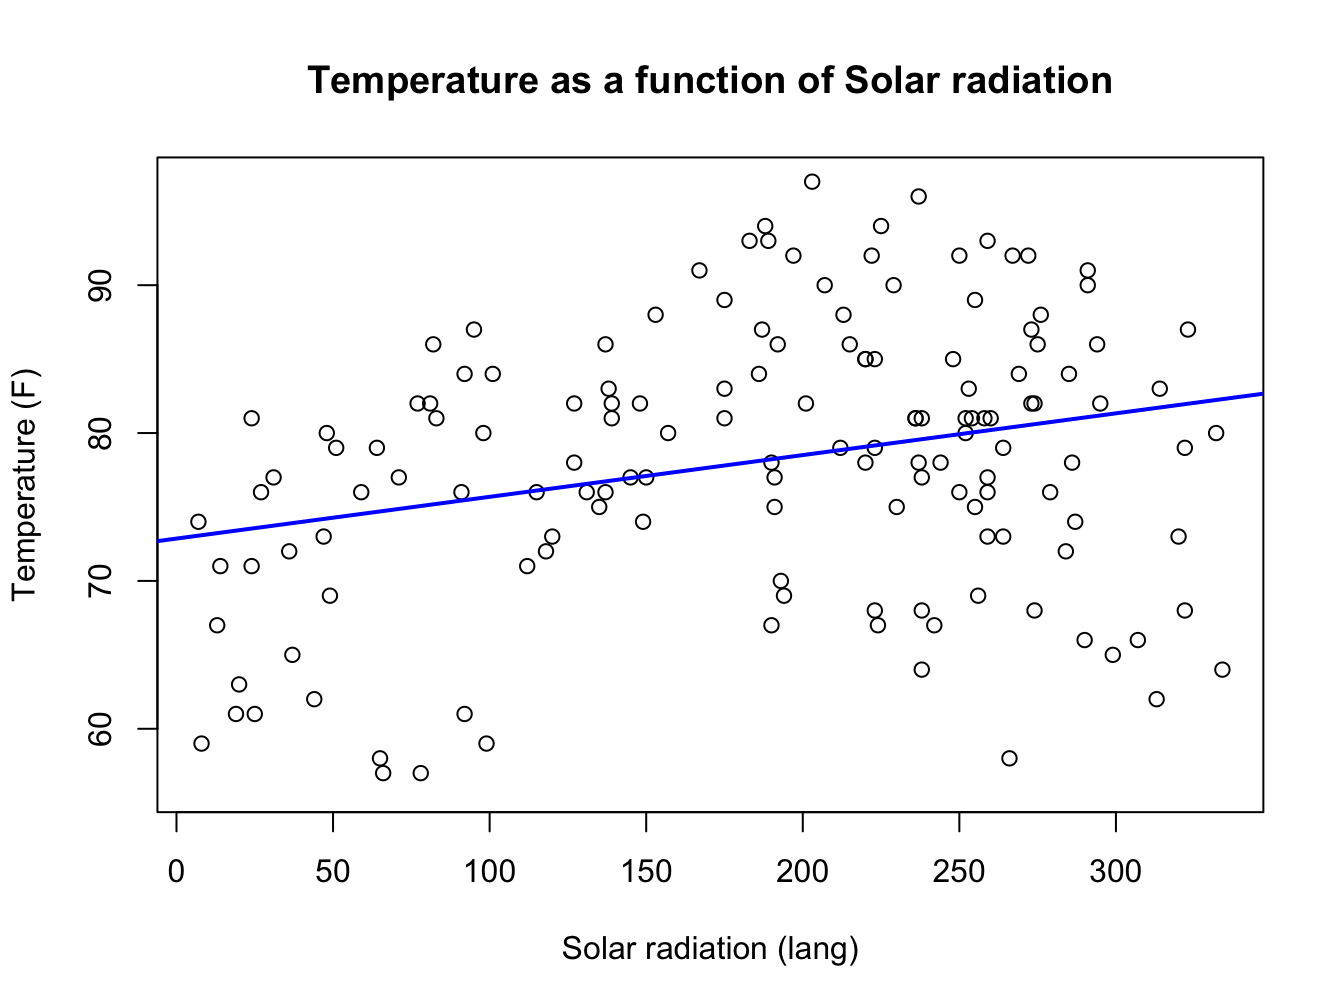
\includegraphics[width=0.8\linewidth]{davur_ebook_files/figure-latex/airquality-1-1} \end{center}

\textbf{B}

\begin{Shaded}
\begin{Highlighting}[]
\KeywordTok{with}\NormalTok{(airquality, }
        \KeywordTok{boxplot}\NormalTok{(Temp }\OperatorTok{~}\StringTok{ }\NormalTok{Month, }
        \DataTypeTok{main =} \StringTok{"Temperature over the months"}\NormalTok{,}
        \DataTypeTok{xlab =} \StringTok{"Month"}\NormalTok{,}
        \DataTypeTok{ylab =} \StringTok{"Temperature (F)"}\NormalTok{))}
\end{Highlighting}
\end{Shaded}

\begin{center}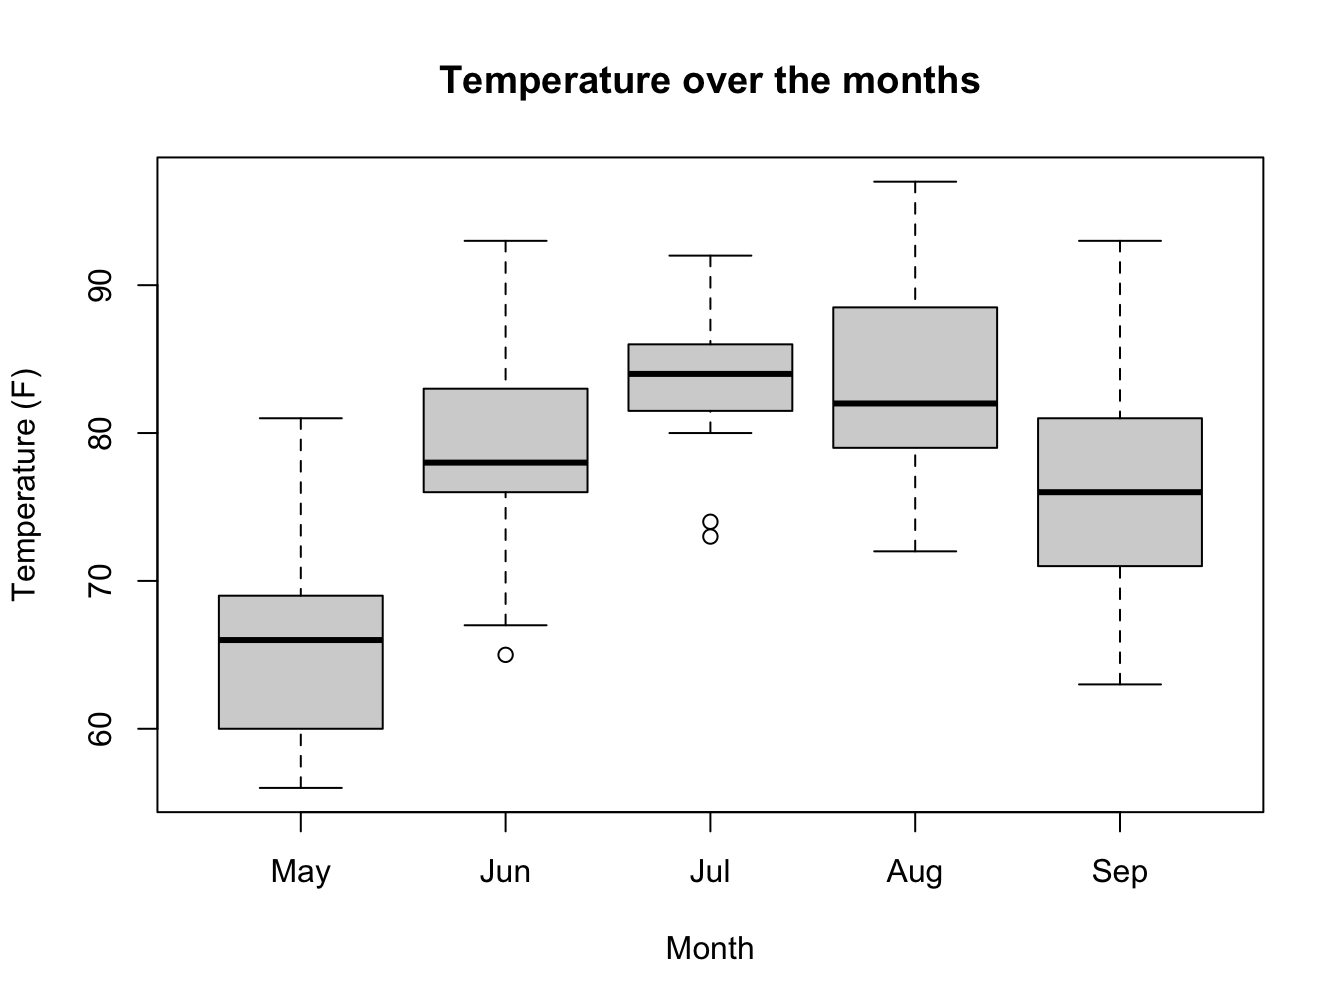
\includegraphics[width=0.8\linewidth]{davur_ebook_files/figure-latex/airquality-2-1} \end{center}

\textbf{C}

\begin{Shaded}
\begin{Highlighting}[]
\CommentTok{#first create Temp Celcius column:}
\CommentTok{#(°F    -    32)    x    5/9 = °C}
\NormalTok{airquality}\OperatorTok{$}\NormalTok{Temp.C <-}\StringTok{ }\NormalTok{(airquality}\OperatorTok{$}\NormalTok{Temp }\OperatorTok{-}\StringTok{ }\DecValTok{32}\NormalTok{) }\OperatorTok{*}\StringTok{ }\DecValTok{5}\OperatorTok{/}\DecValTok{9}
\CommentTok{#get the required data}
\NormalTok{airquality[airquality}\OperatorTok{$}\NormalTok{Temp.C }\OperatorTok{==}\StringTok{ }\KeywordTok{min}\NormalTok{(airquality}\OperatorTok{$}\NormalTok{Temp.C), }\KeywordTok{c}\NormalTok{(}\StringTok{"Temp.C"}\NormalTok{, }\StringTok{"Month"}\NormalTok{, }\StringTok{"Day"}\NormalTok{)]}
\end{Highlighting}
\end{Shaded}

\begin{verbatim}
##     Temp.C Month Day
## 5 13.33333   May   5
\end{verbatim}

\textbf{D}

\begin{Shaded}
\begin{Highlighting}[]
\KeywordTok{hist}\NormalTok{(airquality}\OperatorTok{$}\NormalTok{Wind, }\DataTypeTok{xlab =} \StringTok{"Wind speed (mph)"}\NormalTok{)}
\KeywordTok{abline}\NormalTok{(}\DataTypeTok{v =} \KeywordTok{mean}\NormalTok{(airquality}\OperatorTok{$}\NormalTok{Wind), }\DataTypeTok{col =} \StringTok{"blue"}\NormalTok{, }\DataTypeTok{lwd =} \DecValTok{2}\NormalTok{)}
\KeywordTok{abline}\NormalTok{(}\DataTypeTok{v =} \KeywordTok{median}\NormalTok{(airquality}\OperatorTok{$}\NormalTok{Wind), }\DataTypeTok{col =} \StringTok{"red"}\NormalTok{, }\DataTypeTok{lwd =} \DecValTok{2}\NormalTok{)}
\end{Highlighting}
\end{Shaded}

\begin{center}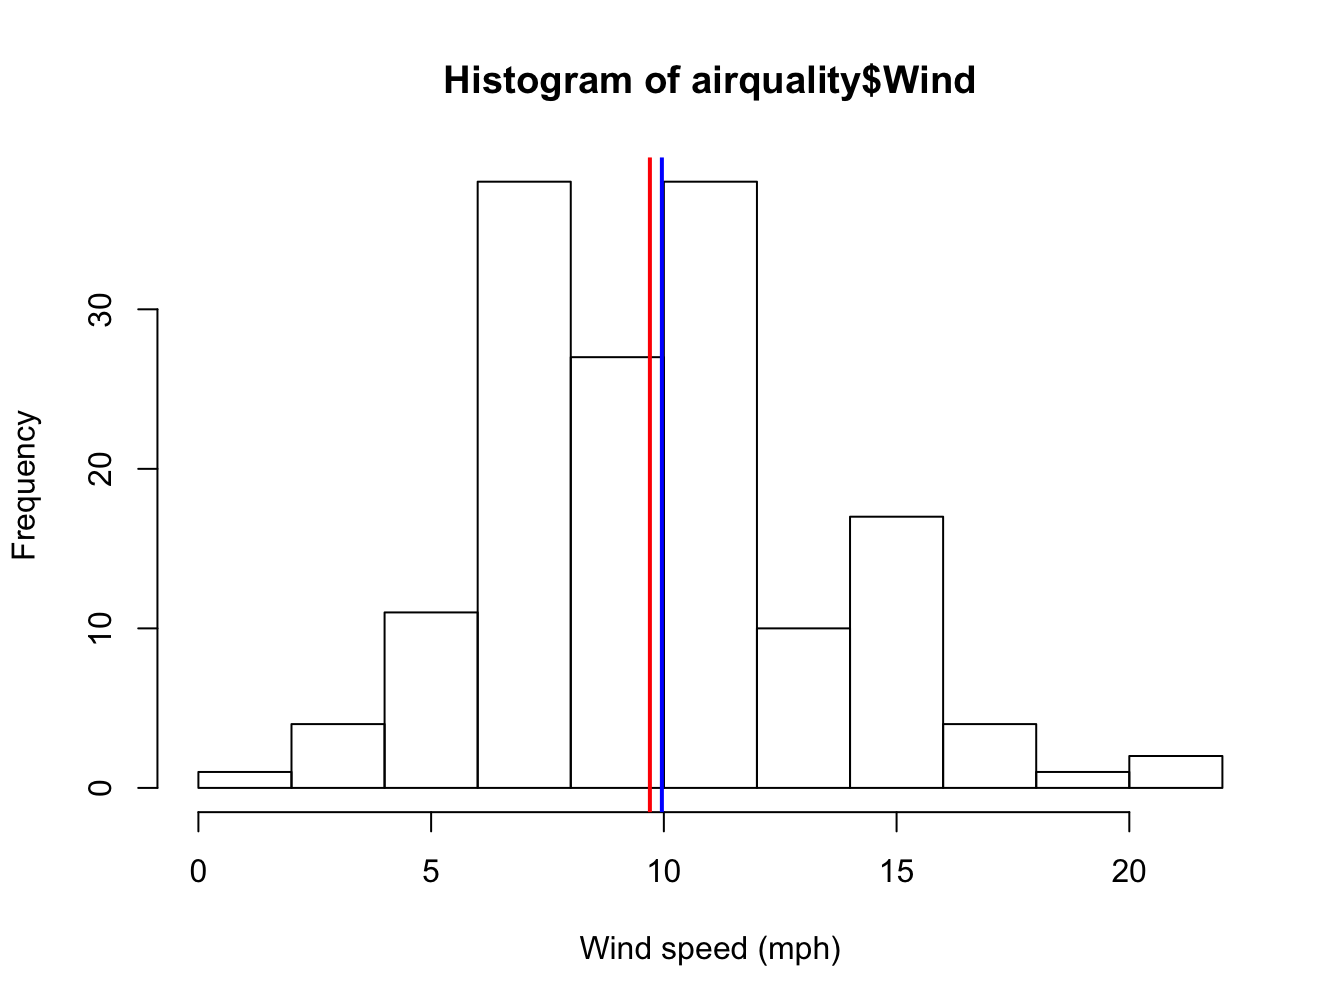
\includegraphics[width=0.8\linewidth]{davur_ebook_files/figure-latex/airquality-4-1} \end{center}

\textbf{E}

\begin{Shaded}
\begin{Highlighting}[]
\KeywordTok{pairs}\NormalTok{(airquality, }\DataTypeTok{panel =}\NormalTok{ panel.smooth)}
\end{Highlighting}
\end{Shaded}

\begin{center}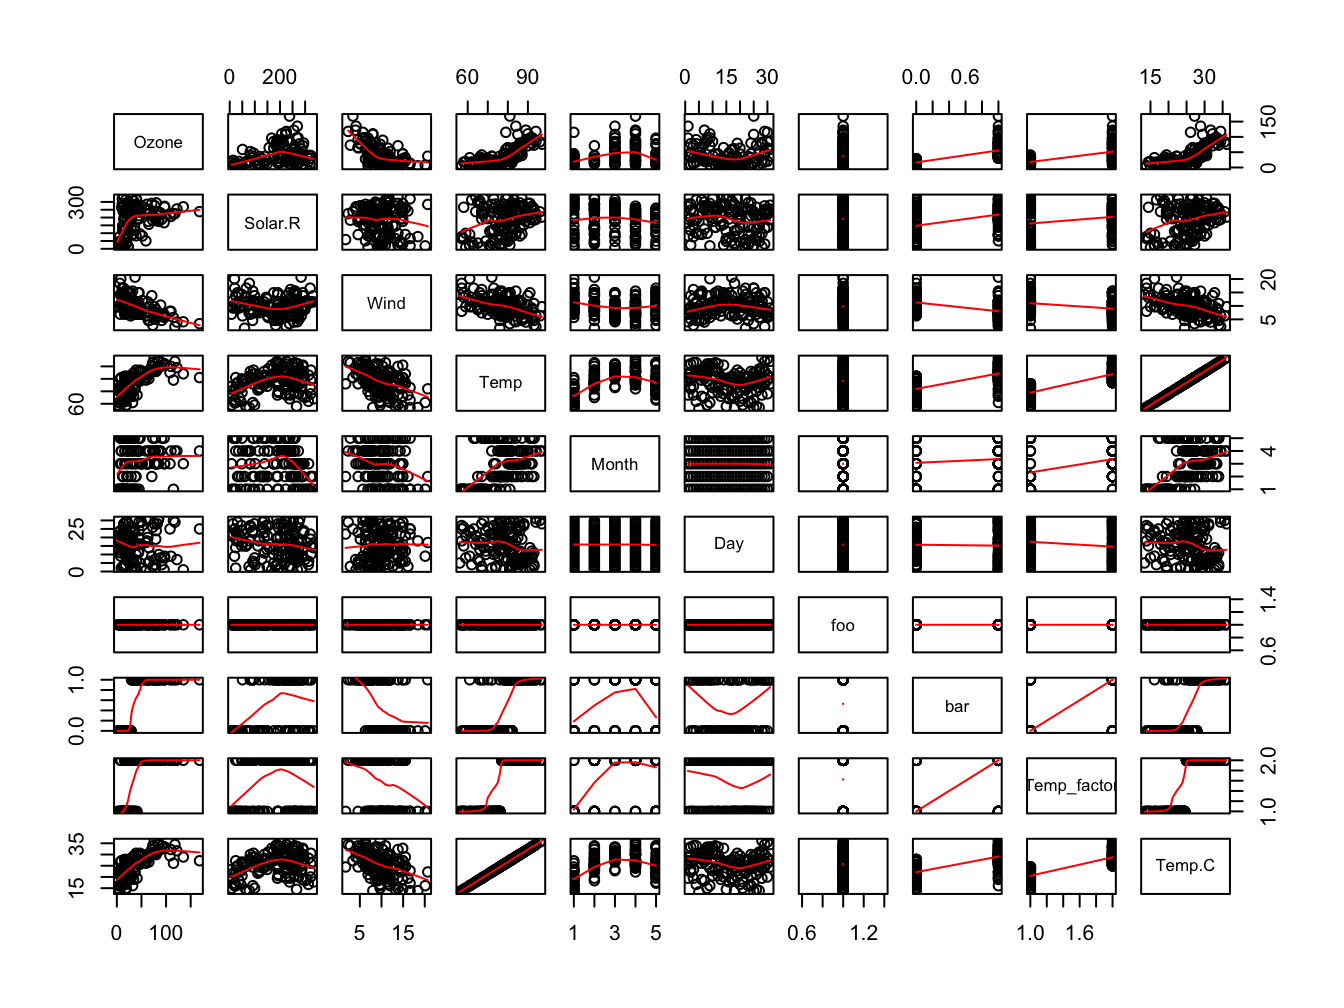
\includegraphics[width=0.8\linewidth]{davur_ebook_files/figure-latex/airquality-5-1} \end{center}

Calculate pairwise correlation.

\begin{Shaded}
\begin{Highlighting}[]
\KeywordTok{cor}\NormalTok{(}\KeywordTok{na.omit}\NormalTok{(airquality))}
\end{Highlighting}
\end{Shaded}

\hypertarget{bird-observations-1}{%
\subsection{Bird observations}\label{bird-observations-1}}

\begin{Shaded}
\begin{Highlighting}[]
\NormalTok{bird_obs <-}\StringTok{ }\KeywordTok{read.table}\NormalTok{(}\StringTok{"data/Observations-Data-2014.csv"}\NormalTok{, }
                                             \DataTypeTok{sep=}\StringTok{";"}\NormalTok{, }
                                             \DataTypeTok{head=}\NormalTok{T, }
                                             \DataTypeTok{na.strings =} \StringTok{""}\NormalTok{, }
                                             \DataTypeTok{quote =} \StringTok{""}\NormalTok{, }
                                             \DataTypeTok{comment.char =} \StringTok{""}\NormalTok{)}
\end{Highlighting}
\end{Shaded}

\textbf{A}

\begin{Shaded}
\begin{Highlighting}[]
\CommentTok{## look at the loaded data structure}
\KeywordTok{str}\NormalTok{(bird_obs)}
\end{Highlighting}
\end{Shaded}

Apparently, all variables are loaded as a factor; also the \texttt{Date.start}, \texttt{Date.end} (should be dates of course), \texttt{Number} (should be \texttt{integer}) and \texttt{Notes} (should be \texttt{character}) columns. In the original column names there are spaces and these are replaced by dots. First column \texttt{Species..} is a serial number and the second \texttt{Species} is the English species name.

\textbf{B}

\begin{Shaded}
\begin{Highlighting}[]
\KeywordTok{nrow}\NormalTok{(bird_obs)}
\end{Highlighting}
\end{Shaded}

\textbf{C}

\begin{Shaded}
\begin{Highlighting}[]
\KeywordTok{class}\NormalTok{(bird_obs}\OperatorTok{$}\NormalTok{Number)}
\end{Highlighting}
\end{Shaded}

\textbf{D}

\begin{Shaded}
\begin{Highlighting}[]
\NormalTok{bird_obs}\OperatorTok{$}\NormalTok{Count <-}\StringTok{ }\KeywordTok{as.integer}\NormalTok{(bird_obs}\OperatorTok{$}\NormalTok{Number)}
\KeywordTok{head}\NormalTok{(bird_obs[, }\KeywordTok{c}\NormalTok{(}\DecValTok{4}\NormalTok{, }\DecValTok{8}\NormalTok{, }\DecValTok{14}\NormalTok{)], }\DataTypeTok{n=}\DecValTok{50}\NormalTok{)}
\end{Highlighting}
\end{Shaded}

\begin{verbatim}
##                    Common.name Number Count
## 1  Greater White-fronted Goose      1     1
## 2  Greater White-fronted Goose      6    58
## 3  Greater White-fronted Goose      1     1
## 4  Greater White-fronted Goose      1     1
## 5  Greater White-fronted Goose      2    22
## 6                   Snow Goose      1     1
## 7                 Ross's Goose      1     1
## 8                 Ross's Goose      1     1
## 9                 Ross's Goose      1     1
## 10                Ross's Goose      1     1
## 11                       Brant    3-6    41
## 12                       Brant      1     1
## 13                       Brant    300    43
## 14                       Brant      1     1
## 15                       Brant      3    36
## 16                       Brant      2    22
## 17                       Brant      9    68
## 18              Cackling Goose      3    36
## 19              Cackling Goose      1     1
## 20              Cackling Goose      1     1
## 21              Cackling Goose      1     1
## 22              Cackling Goose      1     1
## 23              Cackling Goose      3    36
## 24              Trumpeter Swan      6    58
## 25                 Tundra Swan      2    22
## 26                 Tundra Swan      1     1
## 27                 Tundra Swan      2    22
## 28                 Tundra Swan      3    36
## 29                 Tundra Swan      2    22
## 30                 Tundra Swan      1     1
## 31                 Tundra Swan      3    36
## 32                 Tundra Swan      1     1
## 33                 Tundra Swan    145    16
## 34                 Tundra Swan      6    58
## 35                 Tundra Swan     18    21
## 36                 Tundra Swan      3    36
## 37                   Wood Duck      1     1
## 38                     Gadwall      2    22
## 39                     Gadwall      3    36
## 40                     Gadwall      1     1
## 41             Eurasian Wigeon      1     1
## 42             American Wigeon      2    22
## 43             American Wigeon      3    36
## 44             American Wigeon      1     1
## 45             American Wigeon      1     1
## 46             American Wigeon    1-2     2
## 47             American Wigeon    2-5    27
## 48            Blue-winged Teal      3    36
## 49            Blue-winged Teal      1     1
## 50            Blue-winged Teal      1     1
\end{verbatim}

The factor \textbf{\emph{levels}} have been converted into integers, not the original values!

\textbf{E}

\begin{Shaded}
\begin{Highlighting}[]
\CommentTok{#read with as.is argument}
\NormalTok{bird_obs <-}\StringTok{ }\KeywordTok{read.table}\NormalTok{(}\StringTok{"data/Observations-Data-2014.csv"}\NormalTok{,}
                                \DataTypeTok{sep=}\StringTok{";"}\NormalTok{,}
                                \DataTypeTok{head=}\NormalTok{T,}
                                \DataTypeTok{na.strings =} \StringTok{""}\NormalTok{,}
                                \DataTypeTok{quote =} \StringTok{""}\NormalTok{,}
                                \DataTypeTok{comment.char =} \StringTok{""}\NormalTok{,}
                                \DataTypeTok{as.is =} \KeywordTok{c}\NormalTok{(}\DecValTok{1}\NormalTok{, }\DecValTok{6}\NormalTok{, }\DecValTok{7}\NormalTok{, }\DecValTok{8}\NormalTok{, }\DecValTok{13}\NormalTok{))}
\KeywordTok{str}\NormalTok{(bird_obs)}
\end{Highlighting}
\end{Shaded}

\begin{verbatim}
## 'data.frame':    2019 obs. of  13 variables:
##  $ Species..  : chr  "4" "4" "4" "4" ...
##  $ Genus      : Factor w/ 166 levels "Accipiter","Agelaius",..: 8 8 8 8 8 38 38 38 38 38 ...
##  $ Species    : Factor w/ 300 levels "aalge","acuta",..: 11 11 11 11 11 42 235 235 235 235 ...
##  $ Common.name: Factor w/ 329 levels "Acorn Woodpecker",..: 121 121 121 121 121 266 239 239 239 239 ...
##  $ CBRC.Review: Factor w/ 3 levels "FALSE","N","Y": 2 2 2 2 2 2 2 2 2 2 ...
##  $ Date.start : chr  "3-Jun-14" "28-Jul-14" "1-Sep-14" "2-Sep-14" ...
##  $ Date.end   : chr  "19-Jun-14" NA NA NA ...
##  $ Number     : chr  "1" "6" "1" "1" ...
##  $ Location   : Factor w/ 980 levels " Coyote Creek Trail San Jose",..: 629 639 169 503 28 673 503 503 420 420 ...
##  $ County     : Factor w/ 9 levels "Alameda","Contra Costa",..: 7 4 9 9 3 9 9 9 4 4 ...
##  $ Observer.1 : Factor w/ 692 levels "A Sojourner",..: 216 351 544 623 333 623 623 623 323 206 ...
##  $ Other.Obs  : Factor w/ 157 levels "Aaron Maizlish",..: NA NA NA NA NA NA NA NA 155 NA ...
##  $ Notes      : chr  "Adult bird seen on golf course grounds with Canada geese!" "Saw 6 along the shoreline of Napa Creek in mid-afternoon.  About 10 Mallards also  swimming nearby and a Caspia"| __truncated__ NA "This is the only bird that matches up with what I saw. Canada like goose, snow white bum prominent, coloring sl"| __truncated__ ...
\end{verbatim}

Convert Number column to Count of integers.

\begin{Shaded}
\begin{Highlighting}[]
\NormalTok{bird_obs}\OperatorTok{$}\NormalTok{Count <-}\StringTok{ }\KeywordTok{as.integer}\NormalTok{(bird_obs}\OperatorTok{$}\NormalTok{Number)}
\end{Highlighting}
\end{Shaded}

\begin{verbatim}
## Warning: NAs introduced by coercion
\end{verbatim}

Note that there are other ways to achieve this, e.g.~the \texttt{colClasses} argument to \texttt{read.table()}.

\textbf{F}

\begin{Shaded}
\begin{Highlighting}[]
\KeywordTok{head}\NormalTok{(bird_obs[, }\KeywordTok{c}\NormalTok{(}\DecValTok{4}\NormalTok{, }\DecValTok{8}\NormalTok{, }\DecValTok{14}\NormalTok{)], }\DataTypeTok{n=}\DecValTok{50}\NormalTok{)}
\KeywordTok{sum}\NormalTok{(}\KeywordTok{is.na}\NormalTok{(bird_obs}\OperatorTok{$}\NormalTok{Count))}
\end{Highlighting}
\end{Shaded}

\textbf{G}

\begin{Shaded}
\begin{Highlighting}[]
\CommentTok{#What is the maximum number of birds in a single sighting?}
\NormalTok{bird_obs[}\KeywordTok{which}\NormalTok{(bird_obs}\OperatorTok{$}\NormalTok{Count }\OperatorTok{==}\StringTok{ }\KeywordTok{max}\NormalTok{(bird_obs}\OperatorTok{$}\NormalTok{Count, }\DataTypeTok{na.rm =}\NormalTok{ T)), ]}
\CommentTok{##OR}
\NormalTok{bird_obs[}\OperatorTok{!}\KeywordTok{is.na}\NormalTok{(bird_obs}\OperatorTok{$}\NormalTok{Count) }\OperatorTok{&}\StringTok{ }\NormalTok{bird_obs}\OperatorTok{$}\NormalTok{Count }\OperatorTok{==}\StringTok{ }\KeywordTok{max}\NormalTok{(bird_obs}\OperatorTok{$}\NormalTok{Count, }\DataTypeTok{na.rm =}\NormalTok{ T), ]}

\CommentTok{#What is the mean sighting count}
\KeywordTok{mean}\NormalTok{(bird_obs}\OperatorTok{$}\NormalTok{Count, }\DataTypeTok{na.rm =}\NormalTok{ T)}

\CommentTok{#What is the median of the sighting count}
\KeywordTok{median}\NormalTok{(bird_obs}\OperatorTok{$}\NormalTok{Count, }\DataTypeTok{na.rm =}\NormalTok{ T)}
\end{Highlighting}
\end{Shaded}

\textbf{H}

\begin{Shaded}
\begin{Highlighting}[]
\KeywordTok{hist}\NormalTok{(bird_obs}\OperatorTok{$}\NormalTok{Count)}
\end{Highlighting}
\end{Shaded}

\begin{center}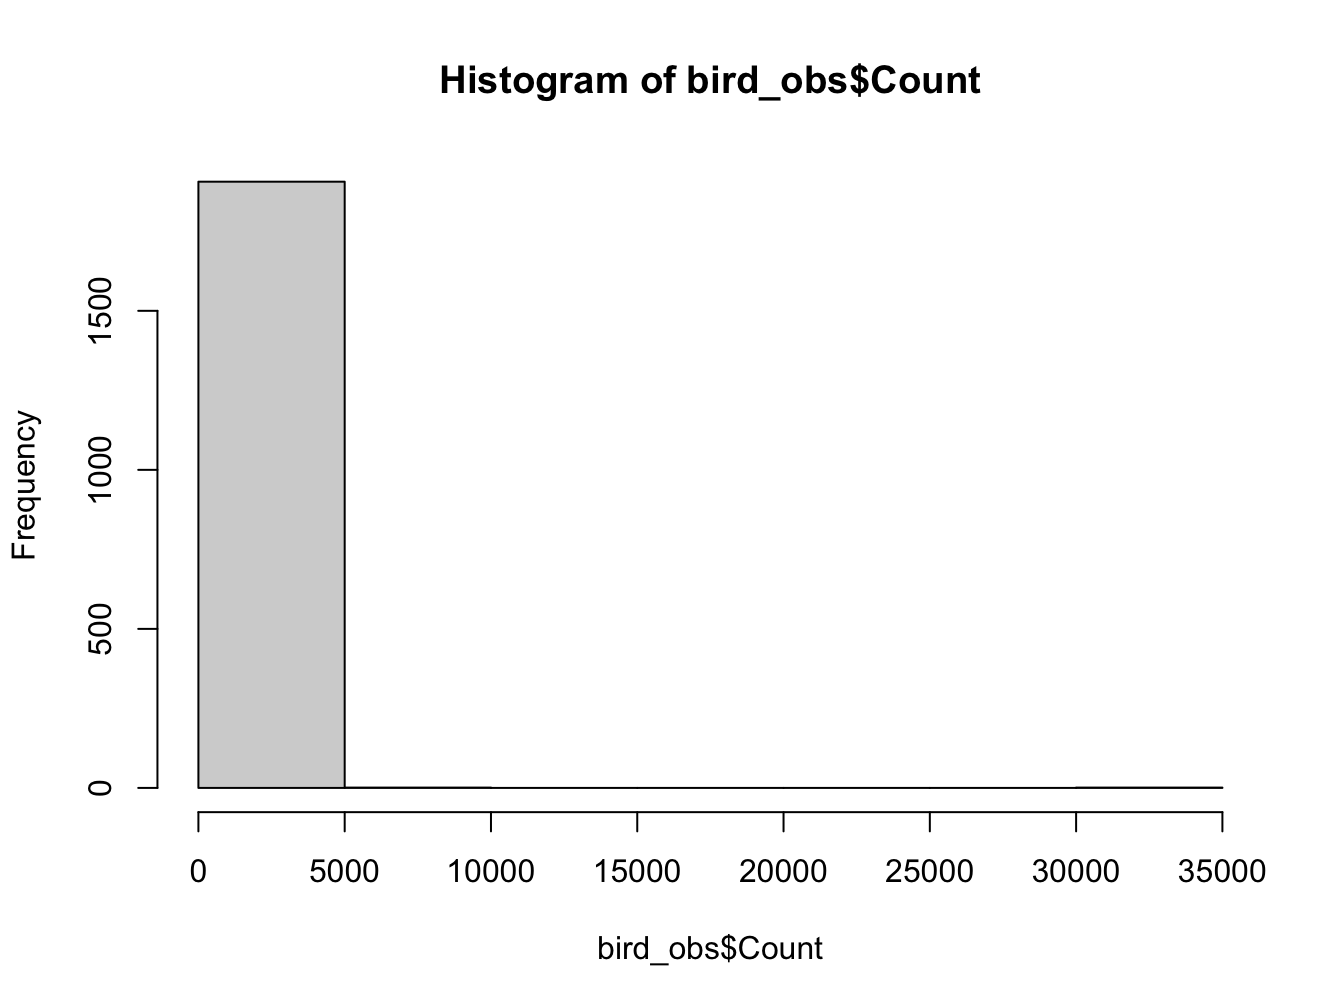
\includegraphics[width=0.8\linewidth]{davur_ebook_files/figure-latex/bird-obs-1-1} \end{center}

Not very helpful, now is it? Try fiddling with the \texttt{breaks} argument.

\begin{Shaded}
\begin{Highlighting}[]
\KeywordTok{plot}\NormalTok{(}\KeywordTok{density}\NormalTok{(bird_obs}\OperatorTok{$}\NormalTok{Count, }\DataTypeTok{na.rm=}\NormalTok{T),}
         \DataTypeTok{main =} \StringTok{"density of Counts"}\NormalTok{)}
\end{Highlighting}
\end{Shaded}

\begin{center}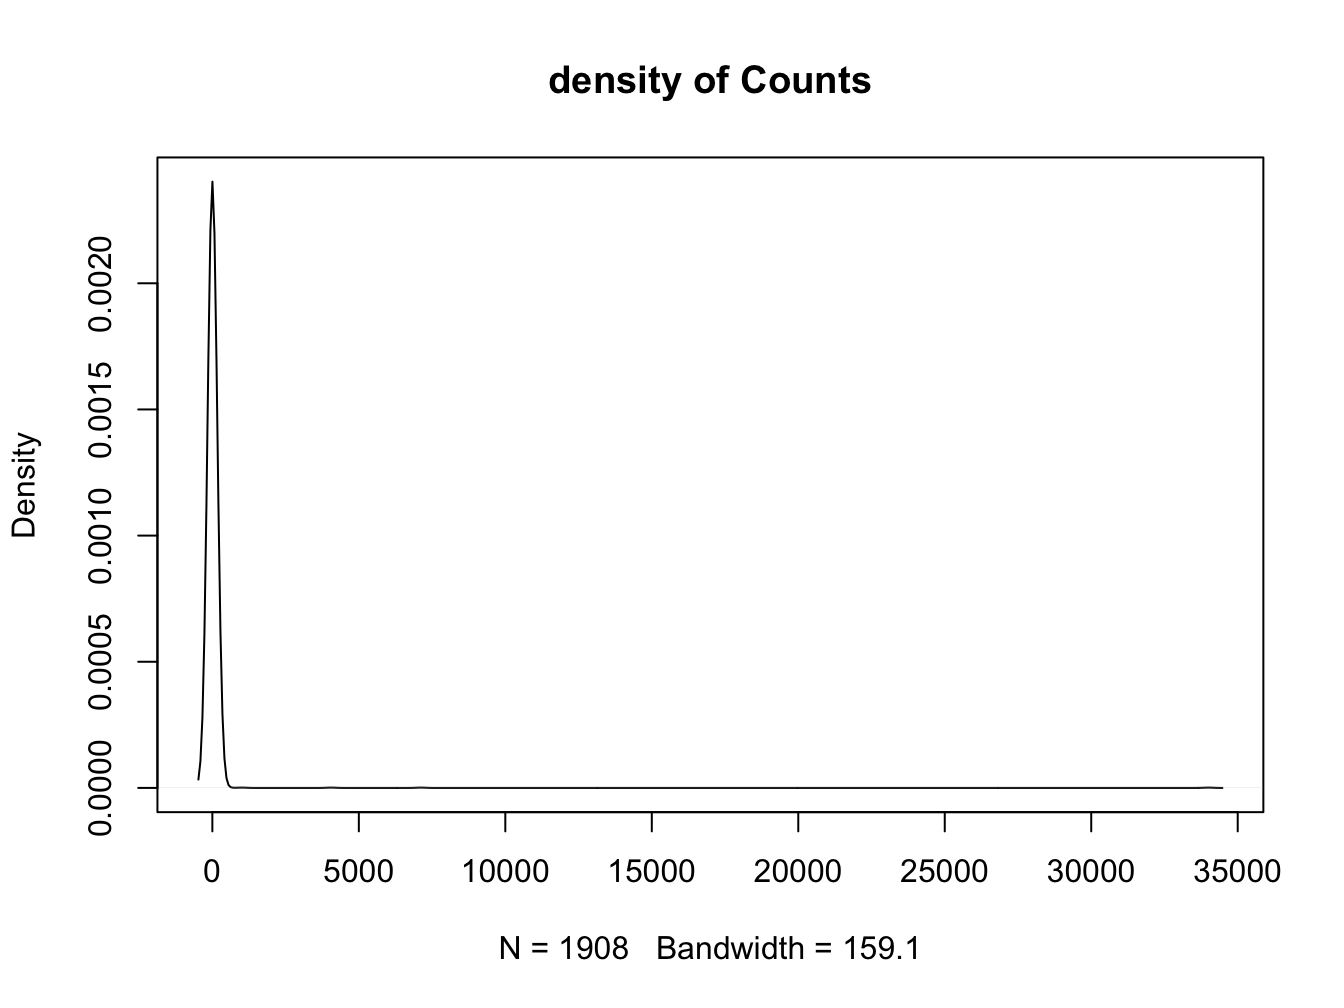
\includegraphics[width=0.8\linewidth]{davur_ebook_files/figure-latex/bird-obs-2-1} \end{center}

Better results with a log transformation (and some coloring)

\begin{Shaded}
\begin{Highlighting}[]
\NormalTok{d <-}\StringTok{ }\KeywordTok{density}\NormalTok{(}\KeywordTok{log}\NormalTok{(bird_obs}\OperatorTok{$}\NormalTok{Count), }\DataTypeTok{na.rm=}\NormalTok{T)}
\KeywordTok{plot}\NormalTok{(d, }\DataTypeTok{main =} \StringTok{"density of log-transformed Counts"}\NormalTok{)}
\KeywordTok{polygon}\NormalTok{(d, }\DataTypeTok{col =} \StringTok{"red"}\NormalTok{, }\DataTypeTok{border =} \StringTok{"blue"}\NormalTok{)}
\end{Highlighting}
\end{Shaded}

\begin{center}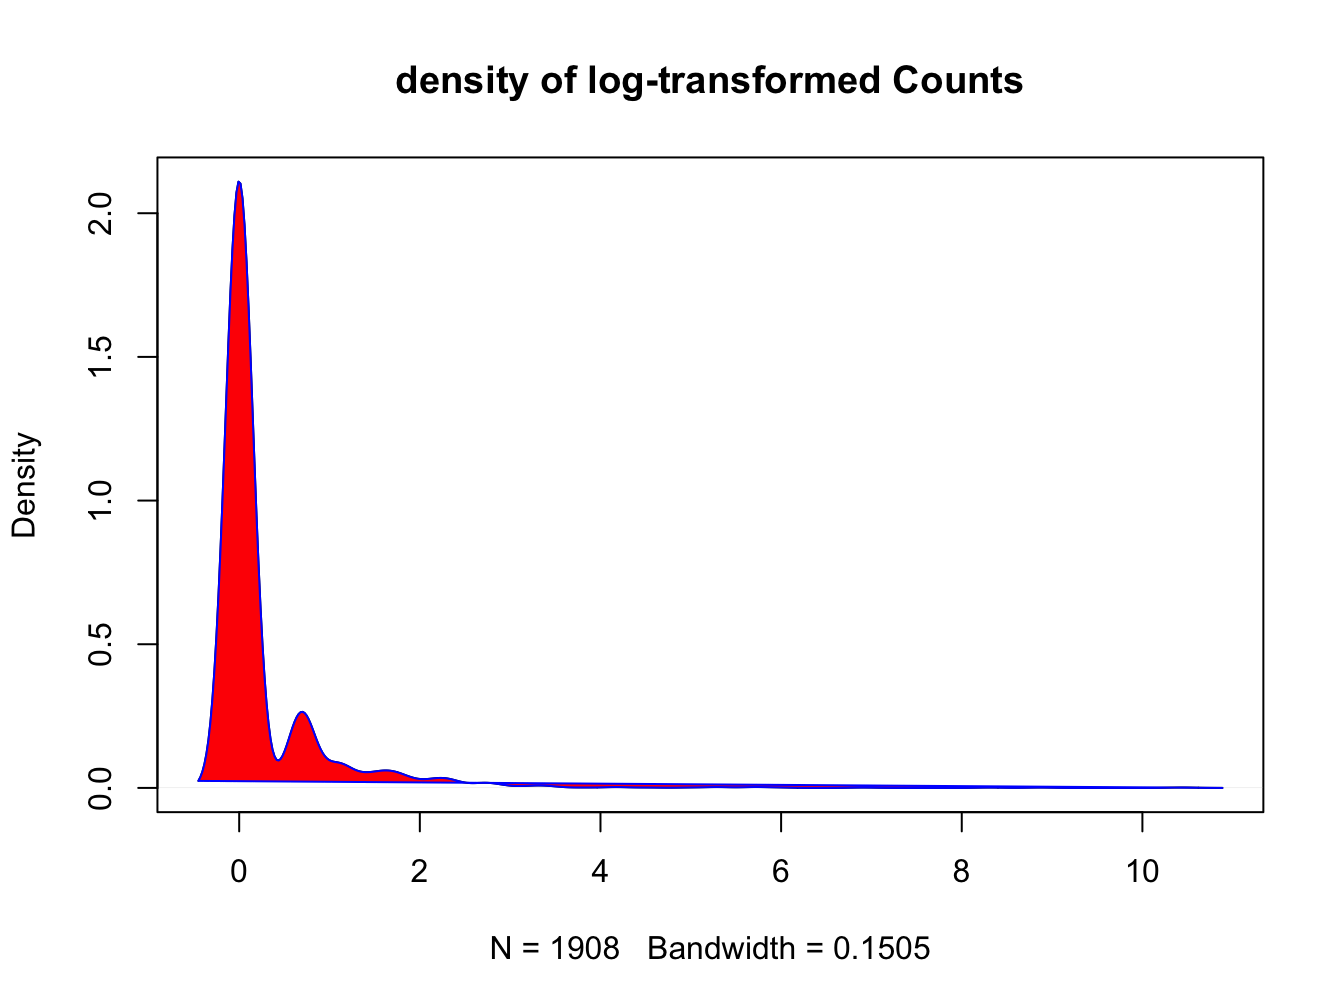
\includegraphics[width=0.8\linewidth]{davur_ebook_files/figure-latex/bird-obs-3-1} \end{center}

\textbf{I}

\begin{Shaded}
\begin{Highlighting}[]
\CommentTok{#How many different species were recorded?}
\KeywordTok{length}\NormalTok{(}\KeywordTok{unique}\NormalTok{(bird_obs}\OperatorTok{$}\NormalTok{Common.name))}

\CommentTok{#How many genera do they constitute?}
\KeywordTok{length}\NormalTok{(}\KeywordTok{unique}\NormalTok{(bird_obs}\OperatorTok{$}\NormalTok{Genus))}

\CommentTok{#What species from the genus "Puffinus" have been observed?}
\CommentTok{#the actual sightings}
\NormalTok{bird_obs[bird_obs}\OperatorTok{$}\NormalTok{Genus }\OperatorTok{==}\StringTok{ "Puffinus"}\NormalTok{, }\KeywordTok{c}\NormalTok{(}\DecValTok{2}\NormalTok{, }\DecValTok{3}\NormalTok{, }\DecValTok{4}\NormalTok{, }\DecValTok{6}\NormalTok{, }\DecValTok{14}\NormalTok{)]}
\CommentTok{#the species}
\KeywordTok{unique}\NormalTok{(bird_obs[bird_obs}\OperatorTok{$}\NormalTok{Genus }\OperatorTok{==}\StringTok{ "Puffinus"}\NormalTok{, }\StringTok{"Common.name"}\NormalTok{])}
\end{Highlighting}
\end{Shaded}

\textbf{J}

\begin{Shaded}
\begin{Highlighting}[]
\CommentTok{#these are the values that need to be rescued:}
\KeywordTok{table}\NormalTok{(bird_obs[}\KeywordTok{is.na}\NormalTok{(bird_obs}\OperatorTok{$}\NormalTok{Count), }\StringTok{"Number"}\NormalTok{])}
\CommentTok{#I suggest you take the lowest of the range-like values: }
\CommentTok{#1-3 becomes 1; 2-3 becomes 2; 100s becomes 100 etc}
\CommentTok{#then do something like}
\NormalTok{tmp <-}\StringTok{ }\NormalTok{bird_obs}\OperatorTok{$}\NormalTok{Number[}\DecValTok{1}\OperatorTok{:}\DecValTok{50}\NormalTok{]}
\NormalTok{tmp}
\KeywordTok{gsub}\NormalTok{(}\StringTok{"(}\CharTok{\textbackslash{}\textbackslash{}}\StringTok{d+)-(}\CharTok{\textbackslash{}\textbackslash{}}\StringTok{d+)"}\NormalTok{, }\StringTok{"}\CharTok{\textbackslash{}\textbackslash{}}\StringTok{1"}\NormalTok{, tmp)}
\end{Highlighting}
\end{Shaded}

\hypertarget{regular-expressions-1}{%
\section{Regular Expressions}\label{regular-expressions-1}}

\hypertarget{restriction-enzymes-1}{%
\subsection{Restriction enzymes}\label{restriction-enzymes-1}}

\textbf{A}

\begin{Shaded}
\begin{Highlighting}[]
\NormalTok{pacI_re <-}\StringTok{ "TTAATTAA"}
\NormalTok{patterns <-}\StringTok{ }\KeywordTok{c}\NormalTok{(}\StringTok{"T\{2\}A\{2\}T\{2\}A\{2\}"}\NormalTok{,}
           \StringTok{"(TTAA)\{2\}"}\NormalTok{, }
           \StringTok{"(T\{2\}A\{2\})\{2\}"}\NormalTok{)}
\ControlFlowTok{for}\NormalTok{(ptrn }\ControlFlowTok{in}\NormalTok{ patterns)\{}
    \KeywordTok{print}\NormalTok{(}\KeywordTok{grepl}\NormalTok{(ptrn, pacI_re))}
\NormalTok{\}}
\end{Highlighting}
\end{Shaded}

\textbf{B}

\begin{Shaded}
\begin{Highlighting}[]
\NormalTok{sfiI_re <-}\StringTok{ "GGCCACGTAGGCC"}
\NormalTok{patterns <-}\StringTok{ }\KeywordTok{c}\NormalTok{(}\StringTok{"G\{2\}C\{2\}[GATC]\{5\}G\{2\}C\{2\}"}\NormalTok{,}
           \StringTok{"GGCC[GATC]\{5\}GGCC"}\NormalTok{, }
           \StringTok{"[GC]\{4\}[GATC]\{5\}[GC]\{4\}"}\NormalTok{) }\CommentTok{#last one is less specific!}
\ControlFlowTok{for}\NormalTok{(ptrn }\ControlFlowTok{in}\NormalTok{ patterns)\{}
    \KeywordTok{print}\NormalTok{(}\KeywordTok{grepl}\NormalTok{(ptrn, sfiI_re))}
\NormalTok{\}}
\end{Highlighting}
\end{Shaded}

\hypertarget{prosite-patterns-1}{%
\subsection{Prosite Patterns}\label{prosite-patterns-1}}

\textbf{A}

PS00211:\\
``{[}LIVMFYC{]}-{[}SA{]}-{[}SAPGLVFYKQH{]}-G-{[}DENQMW{]}-{[}KRQASPCLIMFW{]}-{[}KRNQSTAVM{]}-{[}KRACLVM{]}-{[}LIVMFYPAN{]}-\{PHY\}-{[}LIVMFW{]}-{[}SAGCLIVP{]}-\{FYWHP\}-\{KRHP\}-{[}LIVMFYWSTA{]}.''

\begin{Shaded}
\begin{Highlighting}[]
\NormalTok{PS00211<-}\StringTok{ "[LIVMFYC][SA][SAPGLVFYKQH]G[DENQMW][KRQASPCLIMFW][KRNQSTAVM][KRACLVM][LIVMFYPAN][^PHY][LIVMFW][SAGCLIVP][^FYWHP][^KRHP][LIVMFYWSTA]"}
\end{Highlighting}
\end{Shaded}

\textbf{B}

PS00018:
``D-\{W\}-{[}DNS{]}-\{ILVFYW\}-{[}DENSTG{]}-{[}DNQGHRK{]}-\{GP\}-{[}LIVMC{]}-{[}DENQSTAGC{]}-x(2)- {[}DE{]}-{[}LIVMFYW{]}.''

\begin{Shaded}
\begin{Highlighting}[]
\NormalTok{PS00018 <-}\StringTok{ "D[^W][DNS][^ILVFYW][DENSTG][DNQGHRK][^GP][LIVMC][DENQSTAGC].\{2\} [DE][LIVMFYW]"}
\end{Highlighting}
\end{Shaded}

\hypertarget{fasta-headers-1}{%
\subsection{Fasta Headers}\label{fasta-headers-1}}

\begin{Shaded}
\begin{Highlighting}[]
\KeywordTok{library}\NormalTok{(stringr)}
\NormalTok{fasta_headers <-}\StringTok{ }\KeywordTok{readLines}\NormalTok{(}\StringTok{"./data/fasta_headers.txt"}\NormalTok{)}
\end{Highlighting}
\end{Shaded}

\textbf{A}

\begin{Shaded}
\begin{Highlighting}[]
\KeywordTok{str_match}\NormalTok{(fasta_headers, }\StringTok{"}\CharTok{\textbackslash{}\textbackslash{}}\StringTok{[(.+)}\CharTok{\textbackslash{}\textbackslash{}}\StringTok{]"}\NormalTok{)[, }\DecValTok{2}\NormalTok{]}
\KeywordTok{str_match}\NormalTok{(fasta_headers, }\StringTok{"}\CharTok{\textbackslash{}\textbackslash{}}\StringTok{[([[:alpha:]]+ [[:alpha:]]+) ?(.+)?}\CharTok{\textbackslash{}\textbackslash{}}\StringTok{]"}\NormalTok{)[, }\DecValTok{2}\NormalTok{]}
\end{Highlighting}
\end{Shaded}

\textbf{B}

\begin{Shaded}
\begin{Highlighting}[]
\KeywordTok{str_match}\NormalTok{(fasta_headers, }\StringTok{">([[:alpha:]]\{2,3\}}\CharTok{\textbackslash{}\textbackslash{}}\StringTok{|}\CharTok{\textbackslash{}\textbackslash{}}\StringTok{w+)}\CharTok{\textbackslash{}\textbackslash{}}\StringTok{|"}\NormalTok{)[, }\DecValTok{2}\NormalTok{]}
\end{Highlighting}
\end{Shaded}

\textbf{C}

\begin{Shaded}
\begin{Highlighting}[]
\KeywordTok{str_match}\NormalTok{(fasta_headers, }\StringTok{">.+}\CharTok{\textbackslash{}\textbackslash{}}\StringTok{| (.+?) }\CharTok{\textbackslash{}\textbackslash{}}\StringTok{["}\NormalTok{)[, }\DecValTok{2}\NormalTok{]}
\end{Highlighting}
\end{Shaded}

\hypertarget{scripting-2}{%
\section{Scripting}\label{scripting-2}}

\hypertarget{illegal-reproductions-1}{%
\subsection{Illegal reproductions}\label{illegal-reproductions-1}}

\hypertarget{the-mean-1}{%
\subsubsection*{The mean}\label{the-mean-1}}
\addcontentsline{toc}{subsubsection}{The mean}

\begin{Shaded}
\begin{Highlighting}[]
\NormalTok{my_mean <-}\StringTok{ }\ControlFlowTok{function}\NormalTok{(x) \{}
        \KeywordTok{sum}\NormalTok{(x, }\DataTypeTok{na.rm =}\NormalTok{ T) }\OperatorTok{/}\StringTok{ }\KeywordTok{length}\NormalTok{(x)}
\NormalTok{\}}
\end{Highlighting}
\end{Shaded}

\hypertarget{standard-deviation-1}{%
\subsubsection*{Standard deviation}\label{standard-deviation-1}}
\addcontentsline{toc}{subsubsection}{Standard deviation}

\begin{Shaded}
\begin{Highlighting}[]
\NormalTok{my_sd <-}\StringTok{ }\ControlFlowTok{function}\NormalTok{(x) \{}
        \KeywordTok{sqrt}\NormalTok{(}\KeywordTok{sum}\NormalTok{((x }\OperatorTok{-}\StringTok{ }\KeywordTok{mean}\NormalTok{(x))}\OperatorTok{^}\DecValTok{2}\NormalTok{)}\OperatorTok{/}\NormalTok{(}\KeywordTok{length}\NormalTok{(x)}\OperatorTok{-}\DecValTok{1}\NormalTok{))}
\NormalTok{\}}
\end{Highlighting}
\end{Shaded}

\hypertarget{median-1}{%
\subsubsection*{Median}\label{median-1}}
\addcontentsline{toc}{subsubsection}{Median}

\begin{Shaded}
\begin{Highlighting}[]
\NormalTok{my_median <-}\StringTok{ }\ControlFlowTok{function}\NormalTok{(x) \{}
\NormalTok{        sorted <-}\StringTok{ }\KeywordTok{sort}\NormalTok{(x)}
        \ControlFlowTok{if}\NormalTok{(}\KeywordTok{length}\NormalTok{(x) }\OperatorTok\StringTok{ }\DecValTok{2} \OperatorTok{==}\StringTok{ }\DecValTok{1}\NormalTok{) \{}
                \CommentTok{#uneven length}
\NormalTok{                my_median <-}\StringTok{ }\NormalTok{sorted[}\KeywordTok{ceiling}\NormalTok{(}\KeywordTok{length}\NormalTok{(x)}\OperatorTok{/}\DecValTok{2}\NormalTok{)]}
\NormalTok{        \} }\ControlFlowTok{else}\NormalTok{ \{}
\NormalTok{                my_median <-}\StringTok{ }\NormalTok{(sorted[}\KeywordTok{length}\NormalTok{(x)}\OperatorTok{/}\DecValTok{2}\NormalTok{] }\OperatorTok{+}\StringTok{ }\NormalTok{sorted[(}\KeywordTok{length}\NormalTok{(x)}\OperatorTok{/}\DecValTok{2}\NormalTok{)}\OperatorTok{+}\DecValTok{1}\NormalTok{]) }\OperatorTok{/}\StringTok{ }\DecValTok{2}
\NormalTok{        \}}
        \KeywordTok{return}\NormalTok{(my_median)}
\NormalTok{\}}
\end{Highlighting}
\end{Shaded}

\hypertarget{interquantile-ranges-1}{%
\subsection{Interquantile ranges}\label{interquantile-ranges-1}}

\begin{Shaded}
\begin{Highlighting}[]
\NormalTok{interquantile_range <-}\StringTok{ }\ControlFlowTok{function}\NormalTok{(x, }\DataTypeTok{lower =} \DecValTok{0}\NormalTok{, }\DataTypeTok{upper =} \DecValTok{1}\NormalTok{) \{}
  \ControlFlowTok{if}\NormalTok{ (}\OperatorTok{!}\StringTok{ }\KeywordTok{is.numeric}\NormalTok{(x) }\OperatorTok{|}\StringTok{ }
\StringTok{      }\OperatorTok{!}\StringTok{ }\KeywordTok{is.numeric}\NormalTok{(lower) }\OperatorTok{|}
\StringTok{      }\OperatorTok{!}\StringTok{ }\KeywordTok{is.numeric}\NormalTok{(upper)) \{}
    \KeywordTok{stop}\NormalTok{(}\StringTok{"all three arguments should be numeric"}\NormalTok{)}
\NormalTok{  \}}
\NormalTok{  lower_val <-}\StringTok{ }\KeywordTok{quantile}\NormalTok{(x, }\DataTypeTok{probs =}\NormalTok{ lower)}
\NormalTok{  upper_val <-}\StringTok{ }\KeywordTok{quantile}\NormalTok{(x, }\DataTypeTok{probs =}\NormalTok{ upper)}
\NormalTok{  tmp <-}\StringTok{ }\NormalTok{upper_val }\OperatorTok{-}\StringTok{ }\NormalTok{lower_val}
  \CommentTok{#a named vector is always nice, for acces but also for display purposes}
  \KeywordTok{names}\NormalTok{(tmp) <-}\StringTok{ }\KeywordTok{paste0}\NormalTok{(lower}\OperatorTok{*}\DecValTok{100}\NormalTok{, }\StringTok{"-"}\NormalTok{, upper}\OperatorTok{*}\DecValTok{100}\NormalTok{, }\StringTok{"%"}\NormalTok{)}
\NormalTok{  tmp}
\NormalTok{\}}
\NormalTok{tst <-}\StringTok{ }\KeywordTok{rnorm}\NormalTok{(}\DecValTok{1000}\NormalTok{)}
\KeywordTok{interquantile_range}\NormalTok{(tst) }\CommentTok{# 0 to 1}
\KeywordTok{interquantile_range}\NormalTok{(tst, }\FloatTok{0.25}\NormalTok{, }\FloatTok{0.75}\NormalTok{) }\CommentTok{# custom}
\CommentTok{#interquantile_range("foo") # error!}
\end{Highlighting}
\end{Shaded}

Perform some tests on the arguments to make a robust method: are all arguments numeric?

To test you method, you can compare \texttt{interquantile\_range(some\_vector,\ 0.25,\ 0.75)} with \texttt{IQR(some\_vector)} - they should be the same.

\hypertarget{vector-distance-1}{%
\subsection{Vector distance}\label{vector-distance-1}}

\begin{Shaded}
\begin{Highlighting}[]
\NormalTok{distance <-}\StringTok{ }\ControlFlowTok{function}\NormalTok{(p, q) \{}
    \ControlFlowTok{if}\NormalTok{ (}\OperatorTok{!}\StringTok{ }\KeywordTok{is.numeric}\NormalTok{(p) }\OperatorTok{|}\StringTok{ }\OperatorTok{!}\StringTok{ }\KeywordTok{is.numeric}\NormalTok{(q)) \{}
        \KeywordTok{stop}\NormalTok{(}\StringTok{"non-numeric vectors passed"}\NormalTok{)}
\NormalTok{    \}}
    \ControlFlowTok{if}\NormalTok{ (}\KeywordTok{length}\NormalTok{(p) }\OperatorTok{!=}\StringTok{ }\KeywordTok{length}\NormalTok{(q)) \{}
        \KeywordTok{stop}\NormalTok{(}\StringTok{"vectors have unequal length"}\NormalTok{)}
\NormalTok{    \}}
    \KeywordTok{sqrt}\NormalTok{(}\KeywordTok{sum}\NormalTok{((p }\OperatorTok{-}\StringTok{ }\NormalTok{q)}\OperatorTok{^}\DecValTok{2}\NormalTok{))}
\NormalTok{\}}
\end{Highlighting}
\end{Shaded}

\hypertarget{other-distance-measures-1}{%
\subsubsection*{Other distance measures}\label{other-distance-measures-1}}
\addcontentsline{toc}{subsubsection}{Other distance measures}

\textbf{\texttt{{[}NO\ SOLUTION\ YET{]}}}

\hypertarget{gc-percentage-of-dna-1}{%
\subsection{G/C percentage of DNA}\label{gc-percentage-of-dna-1}}

\begin{Shaded}
\begin{Highlighting}[]
\NormalTok{GC_perc <-}\StringTok{ }\ControlFlowTok{function}\NormalTok{(seq, }\DataTypeTok{strict =} \OtherTok{TRUE}\NormalTok{) \{}
        \ControlFlowTok{if}\NormalTok{ (}\KeywordTok{is.na}\NormalTok{(seq)) \{}
                \KeywordTok{return}\NormalTok{(}\OtherTok{NA}\NormalTok{)}
\NormalTok{        \}}
        \ControlFlowTok{if}\NormalTok{ (}\KeywordTok{length}\NormalTok{(seq) }\OperatorTok{==}\StringTok{ }\DecValTok{0}\NormalTok{) \{}
                \KeywordTok{return}\NormalTok{(}\DecValTok{0}\NormalTok{)}
\NormalTok{        \}}
\NormalTok{        seq.split <-}\StringTok{ }\KeywordTok{strsplit}\NormalTok{(seq, }\StringTok{""}\NormalTok{)[[}\DecValTok{1}\NormalTok{]]}
\NormalTok{        gc.count <-}\StringTok{ }\DecValTok{0}
\NormalTok{        anom.count <-}\StringTok{ }\DecValTok{0}
        \ControlFlowTok{for}\NormalTok{ (n }\ControlFlowTok{in}\NormalTok{ seq.split) \{}
                \ControlFlowTok{if}\NormalTok{ (}\KeywordTok{length}\NormalTok{(}\KeywordTok{grep}\NormalTok{(}\StringTok{"[GATUCgatuc]"}\NormalTok{, n)) }\OperatorTok{>}\StringTok{ }\DecValTok{0}\NormalTok{) \{}
                        \ControlFlowTok{if}\NormalTok{ (n }\OperatorTok{==}\StringTok{ "G"} \OperatorTok{||}\StringTok{ }\NormalTok{n }\OperatorTok{==}\StringTok{ "C"}\NormalTok{) \{}
\NormalTok{                                gc.count <-}\StringTok{ }\NormalTok{gc.count }\OperatorTok{+}\StringTok{ }\DecValTok{1}
\NormalTok{                        \}}
\NormalTok{                \} }\ControlFlowTok{else}\NormalTok{ \{}
                        \ControlFlowTok{if}\NormalTok{ (strict) \{}
                                \KeywordTok{stop}\NormalTok{(}\KeywordTok{paste}\NormalTok{(}\StringTok{"Illegal character"}\NormalTok{, n))}
\NormalTok{                        \} }\ControlFlowTok{else}\NormalTok{ \{}
\NormalTok{                                anom.count <-}\StringTok{ }\NormalTok{anom.count }\OperatorTok{+}\StringTok{ }\DecValTok{1}     
\NormalTok{                        \}}
\NormalTok{                \}}
\NormalTok{        \}}
        \CommentTok{##return perc}
        \CommentTok{##print(gc.count)}
        \ControlFlowTok{if}\NormalTok{ (anom.count }\OperatorTok{>}\StringTok{ }\DecValTok{0}\NormalTok{) \{}
\NormalTok{                anom.perc <-}\StringTok{ }\NormalTok{anom.count }\OperatorTok{/}\StringTok{ }\KeywordTok{nchar}\NormalTok{(seq) }\OperatorTok{*}\StringTok{ }\DecValTok{100}
                \KeywordTok{warning}\NormalTok{(}\KeywordTok{paste}\NormalTok{(}\StringTok{"Non-DNA characters have percentage of"}\NormalTok{, anom.perc))}
\NormalTok{        \}}
        \KeywordTok{return}\NormalTok{(gc.count }\OperatorTok{/}\StringTok{ }\KeywordTok{nchar}\NormalTok{(seq) }\OperatorTok{*}\StringTok{ }\DecValTok{100}\NormalTok{)}
\NormalTok{\}}
\end{Highlighting}
\end{Shaded}

\hypertarget{function-apply-and-its-relatives-1}{%
\section{\texorpdfstring{Function \texttt{apply} and its relatives}{Function apply and its relatives}}\label{function-apply-and-its-relatives-1}}

\hypertarget{whale-selenium-1}{%
\subsection{Whale selenium}\label{whale-selenium-1}}

\begin{Shaded}
\begin{Highlighting}[]
\NormalTok{whale_sel_url <-}\StringTok{ "https://raw.githubusercontent.com/MichielNoback/davur1/gh-pages/exercises/data/whale_selenium.txt"}
\NormalTok{whale_selenium <-}\StringTok{ }\KeywordTok{read.table}\NormalTok{(whale_sel_url,}
        \DataTypeTok{header =}\NormalTok{ T,}
        \DataTypeTok{row.names =} \DecValTok{1}\NormalTok{)}
\end{Highlighting}
\end{Shaded}

\textbf{A}

\begin{Shaded}
\begin{Highlighting}[]
\KeywordTok{apply}\NormalTok{(}\DataTypeTok{X =}\NormalTok{ whale_selenium, }\DataTypeTok{MARGIN =} \DecValTok{2}\NormalTok{, }\DataTypeTok{FUN =}\NormalTok{ mean)}
\end{Highlighting}
\end{Shaded}

\textbf{B}

\begin{Shaded}
\begin{Highlighting}[]
\KeywordTok{apply}\NormalTok{(}\DataTypeTok{X =}\NormalTok{ whale_selenium, }\DataTypeTok{MARGIN =} \DecValTok{2}\NormalTok{, }\DataTypeTok{FUN =}\NormalTok{ sd)}
\end{Highlighting}
\end{Shaded}

\textbf{C}

\begin{Shaded}
\begin{Highlighting}[]
\NormalTok{my.sem <-}\StringTok{ }\ControlFlowTok{function}\NormalTok{(x) \{}
\NormalTok{        sem <-}\StringTok{ }\KeywordTok{sd}\NormalTok{(x) }\OperatorTok{/}\StringTok{ }\KeywordTok{sqrt}\NormalTok{(}\KeywordTok{length}\NormalTok{(x))}
\NormalTok{\}}
\KeywordTok{apply}\NormalTok{(}\DataTypeTok{X =}\NormalTok{ whale_selenium, }\DataTypeTok{MARGIN =} \DecValTok{2}\NormalTok{, }\DataTypeTok{FUN =}\NormalTok{ my.sem)}
\end{Highlighting}
\end{Shaded}

\textbf{D}

\begin{Shaded}
\begin{Highlighting}[]
\NormalTok{whale_selenium}\OperatorTok{$}\NormalTok{ratio <-}\StringTok{ }\KeywordTok{apply}\NormalTok{(}\DataTypeTok{X =}\NormalTok{ whale_selenium, }
            \DataTypeTok{MARGIN =} \DecValTok{1}\NormalTok{, }
            \DataTypeTok{FUN =} \ControlFlowTok{function}\NormalTok{(x)\{}
\NormalTok{                    x[}\DecValTok{2}\NormalTok{] }\OperatorTok{/}\StringTok{ }\NormalTok{x[}\DecValTok{1}\NormalTok{]}
\NormalTok{            \})}
\KeywordTok{hist}\NormalTok{(whale_selenium}\OperatorTok{$}\NormalTok{ratio,}
         \DataTypeTok{xlab =} \StringTok{"Tooth / Liver Selenium ratio"}\NormalTok{,}
         \DataTypeTok{main =} \StringTok{"Histogram of Tooth / Liver Selenium ratios"}\NormalTok{)}
\end{Highlighting}
\end{Shaded}

\begin{center}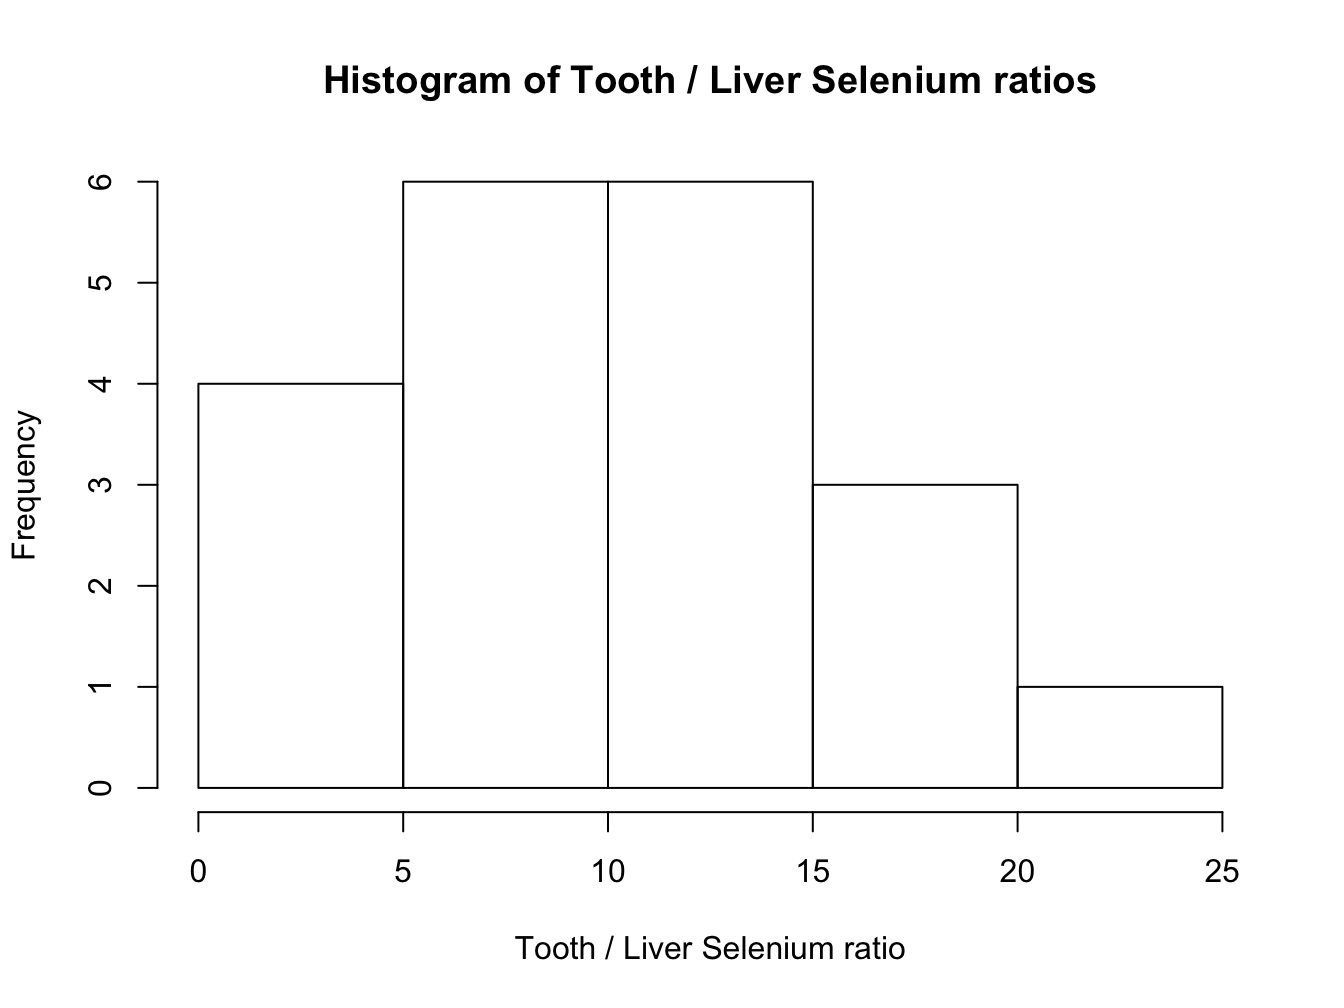
\includegraphics[width=0.8\linewidth]{davur_ebook_files/figure-latex/whale-selenium-hist-1} \end{center}

\textbf{E}

Inline expressions are like this: 15.4 MpH.

\hypertarget{chickweight-1}{%
\subsection{ChickWeight}\label{chickweight-1}}

This exercise revolves around the \texttt{ChickWeight} dataset of the built-in \texttt{datasets} package.

\textbf{A}

\begin{Shaded}
\begin{Highlighting}[]
\CommentTok{#MANY WAYS TO GET THERE}
\KeywordTok{length}\NormalTok{(}\KeywordTok{split}\NormalTok{(ChickWeight, ChickWeight}\OperatorTok{$}\NormalTok{Chick))}
\end{Highlighting}
\end{Shaded}

\begin{verbatim}
## [1] 50
\end{verbatim}

\begin{Shaded}
\begin{Highlighting}[]
\CommentTok{#OR}
\KeywordTok{sum}\NormalTok{(}\KeywordTok{tapply}\NormalTok{(ChickWeight}\OperatorTok{$}\NormalTok{Diet, ChickWeight}\OperatorTok{$}\NormalTok{Chick, }\DataTypeTok{FUN =} \ControlFlowTok{function}\NormalTok{(x)\{}\DecValTok{1}\NormalTok{\}))}
\end{Highlighting}
\end{Shaded}

\begin{verbatim}
## [1] 50
\end{verbatim}

\begin{Shaded}
\begin{Highlighting}[]
\CommentTok{#OR}
\KeywordTok{length}\NormalTok{(}\KeywordTok{unique}\NormalTok{(ChickWeight}\OperatorTok{$}\NormalTok{Chick))}
\end{Highlighting}
\end{Shaded}

\begin{verbatim}
## [1] 50
\end{verbatim}

\begin{Shaded}
\begin{Highlighting}[]
\CommentTok{#OR}
\KeywordTok{nrow}\NormalTok{(}\KeywordTok{aggregate}\NormalTok{(}\DataTypeTok{x =}\NormalTok{ ChickWeight, }\DataTypeTok{by =} \KeywordTok{list}\NormalTok{(ChickWeight}\OperatorTok{$}\NormalTok{Chick), }\DataTypeTok{FUN =} \ControlFlowTok{function}\NormalTok{(x)\{x\}))}
\end{Highlighting}
\end{Shaded}

\begin{verbatim}
## [1] 50
\end{verbatim}

\textbf{B}

\begin{Shaded}
\begin{Highlighting}[]
\KeywordTok{aggregate}\NormalTok{(}\DataTypeTok{formula =}\NormalTok{ weight }\OperatorTok{~}\StringTok{ }\NormalTok{Diet, }\DataTypeTok{data=}\NormalTok{ChickWeight, }\DataTypeTok{FUN =}\NormalTok{ mean, }\DataTypeTok{na.rm =}\NormalTok{ T)}
\end{Highlighting}
\end{Shaded}

\begin{verbatim}
##   Diet   weight
## 1    1 102.6455
## 2    2 122.6167
## 3    3 142.9500
## 4    4 135.2627
\end{verbatim}

\begin{Shaded}
\begin{Highlighting}[]
\CommentTok{#OR}
\KeywordTok{aggregate}\NormalTok{(}\DataTypeTok{x =}\NormalTok{ ChickWeight}\OperatorTok{$}\NormalTok{weight, }\DataTypeTok{by =} \KeywordTok{list}\NormalTok{(}\DataTypeTok{Diet =}\NormalTok{ ChickWeight}\OperatorTok{$}\NormalTok{Diet), }\DataTypeTok{FUN =}\NormalTok{ mean, }\DataTypeTok{na.rm =}\NormalTok{ T)}
\end{Highlighting}
\end{Shaded}

\begin{verbatim}
##   Diet        x
## 1    1 102.6455
## 2    2 122.6167
## 3    3 142.9500
## 4    4 135.2627
\end{verbatim}

\textbf{C}

\begin{Shaded}
\begin{Highlighting}[]
\KeywordTok{coplot}\NormalTok{(weight }\OperatorTok{~}\StringTok{ }\NormalTok{Time }\OperatorTok{|}\StringTok{ }\NormalTok{Diet, }\DataTypeTok{data =}\NormalTok{ ChickWeight, }\DataTypeTok{panel =}\NormalTok{ panel.smooth)}
\end{Highlighting}
\end{Shaded}

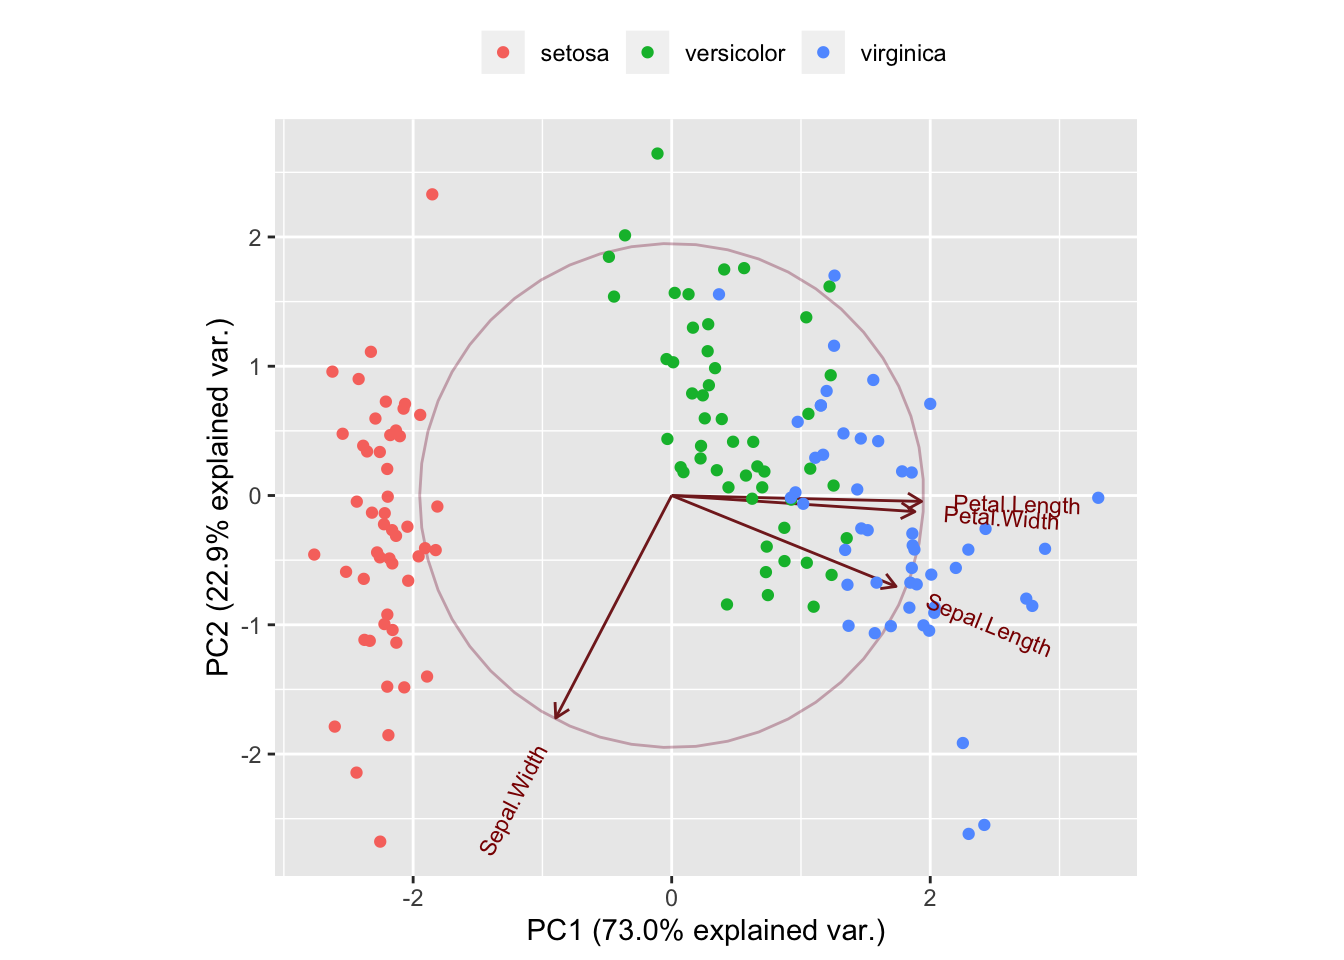
\includegraphics{davur_ebook_files/figure-latex/unnamed-chunk-43-1.pdf}

\textbf{D}

\begin{Shaded}
\begin{Highlighting}[]
\CommentTok{#A naive for-loop here - is this the best solution?}
\NormalTok{ChickWeight}\OperatorTok{$}\NormalTok{weight_gain <-}\StringTok{ }\OtherTok{NA} \CommentTok{#create the column with missing values}
\ControlFlowTok{for}\NormalTok{ (i }\ControlFlowTok{in} \DecValTok{1}\OperatorTok{:}\KeywordTok{nrow}\NormalTok{(ChickWeight)) \{}
        \CommentTok{#skip first row and rows that are preceded by values for another chick}
        \ControlFlowTok{if}\NormalTok{ (i }\OperatorTok{>}\StringTok{ }\DecValTok{1} \OperatorTok{&&}\StringTok{ }\NormalTok{ChickWeight}\OperatorTok{$}\NormalTok{Chick[i] }\OperatorTok{==}\StringTok{ }\NormalTok{ChickWeight}\OperatorTok{$}\NormalTok{Chick[i}\DecValTok{-1}\NormalTok{]) \{}
\NormalTok{                ChickWeight[i, }\StringTok{"weight_gain"}\NormalTok{] <-}\StringTok{ }\NormalTok{ChickWeight}\OperatorTok{$}\NormalTok{weight[i] }\OperatorTok{-}\StringTok{ }\NormalTok{ChickWeight}\OperatorTok{$}\NormalTok{weight[i}\DecValTok{-1}\NormalTok{] }
\NormalTok{        \}}
\NormalTok{\}}
\end{Highlighting}
\end{Shaded}

\textbf{E}

\begin{Shaded}
\begin{Highlighting}[]
\NormalTok{local_file <-}\StringTok{ "ChickWeight_weight_gain.Rdata"}
\KeywordTok{download.file}\NormalTok{(}\KeywordTok{paste0}\NormalTok{(}\StringTok{"https://github.com/MichielNoback/davur1_gitbook/raw/master/data/"}\NormalTok{, local_file), local_file)}
\KeywordTok{load}\NormalTok{(local_file)}
\CommentTok{#attach}
\NormalTok{ChickWeight}\OperatorTok{$}\NormalTok{weight_gain <-}\StringTok{ }\NormalTok{stored.weight.gain}
\end{Highlighting}
\end{Shaded}

\begin{Shaded}
\begin{Highlighting}[]
\KeywordTok{tapply}\NormalTok{(}\DataTypeTok{X =}\NormalTok{ ChickWeight}\OperatorTok{$}\NormalTok{weight_gain, }\DataTypeTok{INDEX =}\NormalTok{ ChickWeight}\OperatorTok{$}\NormalTok{Diet, }\DataTypeTok{FUN =}\NormalTok{ mean, }\DataTypeTok{na.rm =}\NormalTok{ T)}
\CommentTok{#or with aggregate}
\KeywordTok{aggregate}\NormalTok{(}\DataTypeTok{formula =}\NormalTok{ weight_gain }\OperatorTok{~}\StringTok{ }\NormalTok{Diet, }\DataTypeTok{data =}\NormalTok{ ChickWeight, }\DataTypeTok{FUN =}\NormalTok{ median)}
\CommentTok{#or with split and sapply}
\KeywordTok{sapply}\NormalTok{(}\KeywordTok{split}\NormalTok{(ChickWeight[, }\StringTok{"weight_gain"}\NormalTok{], ChickWeight}\OperatorTok{$}\NormalTok{Diet), sd, }\DataTypeTok{na.rm =}\NormalTok{ T)}
\end{Highlighting}
\end{Shaded}

\textbf{F}

\begin{Shaded}
\begin{Highlighting}[]
\KeywordTok{boxplot}\NormalTok{(weight_gain }\OperatorTok{~}\StringTok{ }\NormalTok{Diet, }\DataTypeTok{data =}\NormalTok{ ChickWeight)}
\end{Highlighting}
\end{Shaded}

\begin{center}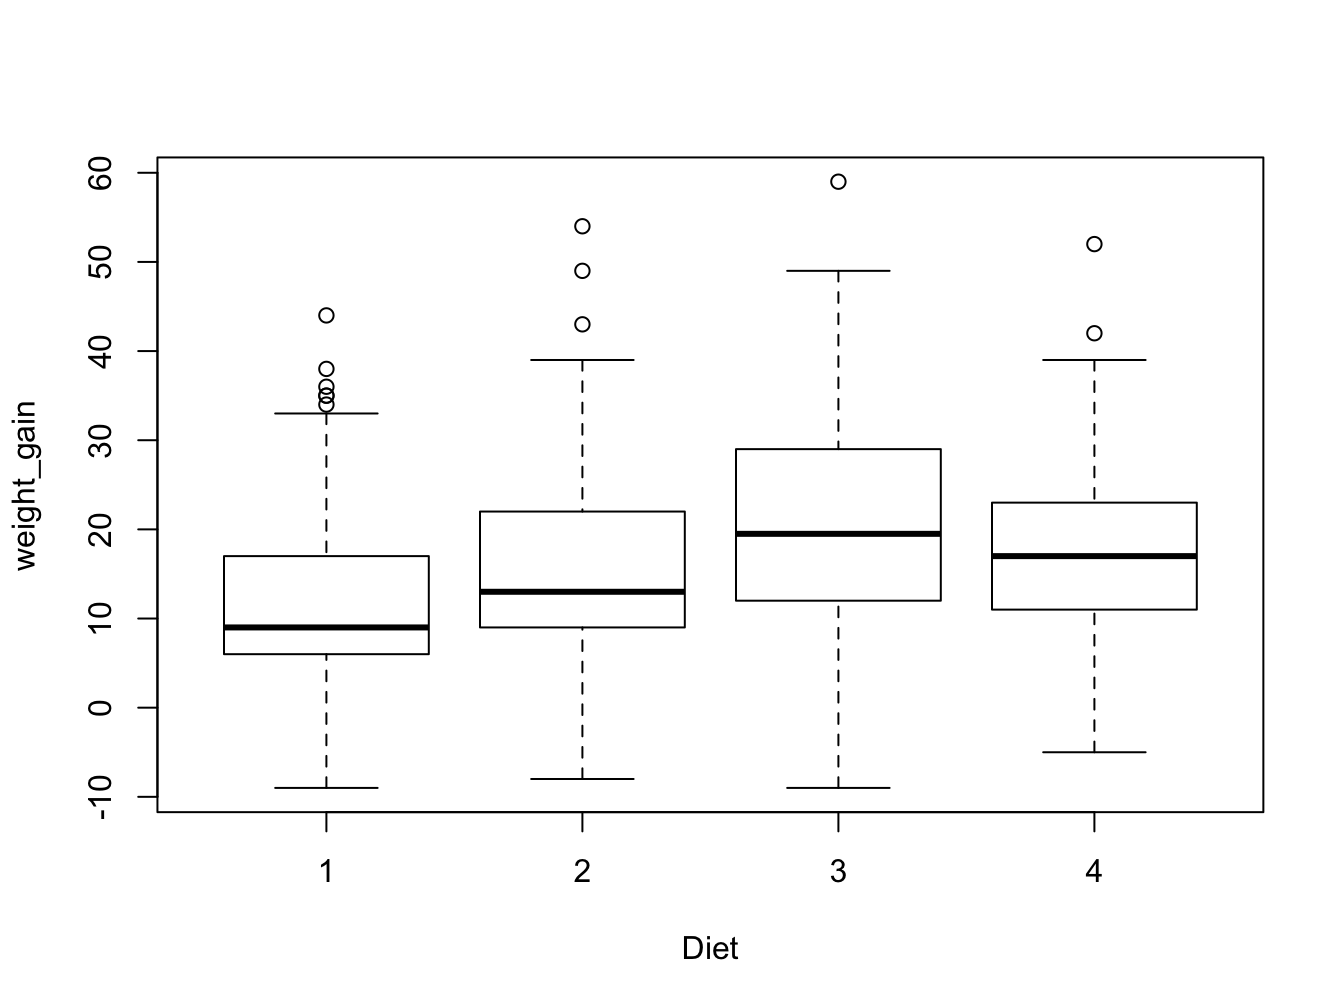
\includegraphics[width=0.8\linewidth]{davur_ebook_files/figure-latex/weight-gain-boxplot-1} \end{center}

\hypertarget{food-constituents-1}{%
\subsection{Food constituents}\label{food-constituents-1}}

\textbf{A}

\begin{Shaded}
\begin{Highlighting}[]
\NormalTok{foods <-}\StringTok{ }\KeywordTok{read.table}\NormalTok{(}
        \StringTok{"https://raw.githubusercontent.com/MichielNoback/davur1_gitbook/master/data/food_constituents.txt"}\NormalTok{, }\DataTypeTok{header =}\NormalTok{ T)}
\end{Highlighting}
\end{Shaded}

\begin{Shaded}
\begin{Highlighting}[]
\KeywordTok{levels}\NormalTok{(foods}\OperatorTok{$}\NormalTok{Type)}
\KeywordTok{table}\NormalTok{(foods}\OperatorTok{$}\NormalTok{Type)}
\end{Highlighting}
\end{Shaded}

\textbf{B}

\begin{Shaded}
\begin{Highlighting}[]
\KeywordTok{mean}\NormalTok{(foods[foods}\OperatorTok{$}\NormalTok{Type }\OperatorTok{==}\StringTok{ "chocolate"}\NormalTok{, }\StringTok{"kcal"}\NormalTok{])}
\end{Highlighting}
\end{Shaded}

\textbf{C}

\begin{Shaded}
\begin{Highlighting}[]
\CommentTok{#aggregate over Type}
\NormalTok{mean.fat <-}\StringTok{ }\KeywordTok{aggregate}\NormalTok{(}\DataTypeTok{formula =}\NormalTok{ fat.total }\OperatorTok{~}\StringTok{ }\NormalTok{Type, }\DataTypeTok{data =}\NormalTok{ foods, }\DataTypeTok{FUN =}\NormalTok{ mean)}
\CommentTok{#order and select first}
\NormalTok{mean.fat[}\KeywordTok{order}\NormalTok{(mean.fat}\OperatorTok{$}\NormalTok{fat.total, }\DataTypeTok{decreasing =}\NormalTok{ T)[}\DecValTok{1}\NormalTok{], ]}
\end{Highlighting}
\end{Shaded}

\textbf{D}

\begin{Shaded}
\begin{Highlighting}[]
\NormalTok{mean.energy <-}\StringTok{ }\KeywordTok{aggregate}\NormalTok{(}\DataTypeTok{formula =}\NormalTok{ kcal }\OperatorTok{~}\StringTok{ }\NormalTok{Type, }\DataTypeTok{data =}\NormalTok{ foods, }\DataTypeTok{FUN =}\NormalTok{ mean)}
\NormalTok{mean.energy[}\KeywordTok{order}\NormalTok{(mean.energy}\OperatorTok{$}\NormalTok{kcal)[}\DecValTok{1}\NormalTok{], ]}
\NormalTok{mean.energy[}\KeywordTok{order}\NormalTok{(mean.energy}\OperatorTok{$}\NormalTok{kcal, }\DataTypeTok{decreasing =}\NormalTok{ T)[}\DecValTok{1}\NormalTok{], ]}
\end{Highlighting}
\end{Shaded}

\textbf{E}

\begin{Shaded}
\begin{Highlighting}[]
\CommentTok{#more verbose means possible; this efficient way demonstrating use of %in%}
\NormalTok{foods}\OperatorTok{$}\NormalTok{solid.state <-}\StringTok{ }\OperatorTok{!}\NormalTok{foods}\OperatorTok{$}\NormalTok{Type }\OperatorTok\StringTok{ }\KeywordTok{c}\NormalTok{(}\StringTok{"milk"}\NormalTok{, }\StringTok{"beverage"}\NormalTok{)}
\KeywordTok{boxplot}\NormalTok{(}\DataTypeTok{formula =}\NormalTok{ carb.sugar }\OperatorTok{~}\StringTok{ }\NormalTok{solid.state, }
                \DataTypeTok{data =}\NormalTok{ foods,}
                \DataTypeTok{main =} \StringTok{"Sugar content of foods categories"}\NormalTok{, }
                \DataTypeTok{names =}\NormalTok{ (}\KeywordTok{c}\NormalTok{(}\StringTok{"Drink"}\NormalTok{, }\StringTok{"Solid"}\NormalTok{)),}
                \DataTypeTok{ylab =} \StringTok{"Sugar (g/100g product)"}\NormalTok{)}
\end{Highlighting}
\end{Shaded}

\begin{center}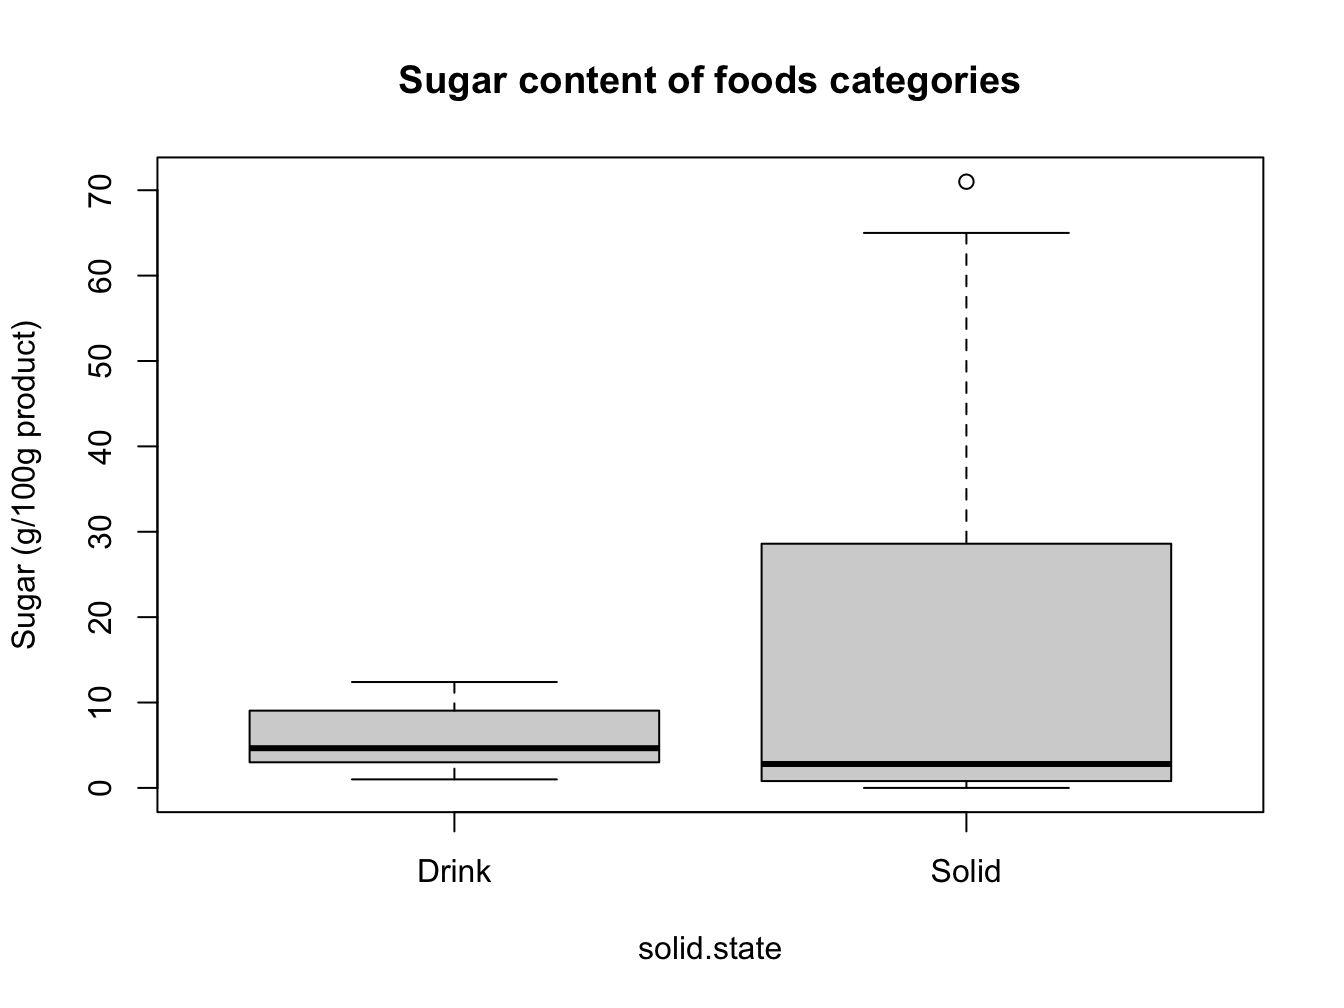
\includegraphics[width=0.8\linewidth]{davur_ebook_files/figure-latex/foods-boxplot-1} \end{center}

\textbf{F}

\[NO WORKED SOLUTION HERE\]

\hypertarget{bird-observations-revisited-1}{%
\subsection{Bird observations revisited}\label{bird-observations-revisited-1}}

\begin{Shaded}
\begin{Highlighting}[]
\NormalTok{bird_obs <-}\StringTok{ }\KeywordTok{read.table}\NormalTok{(}\StringTok{"data/Observations-Data-2014.csv"}\NormalTok{,}
                                \DataTypeTok{sep=}\StringTok{";"}\NormalTok{,}
                                \DataTypeTok{head=}\NormalTok{T,}
                                \DataTypeTok{na.strings =} \StringTok{""}\NormalTok{,}
                                \DataTypeTok{quote =} \StringTok{""}\NormalTok{,}
                                \DataTypeTok{comment.char =} \StringTok{""}\NormalTok{,}
                                \DataTypeTok{as.is =} \KeywordTok{c}\NormalTok{(}\DecValTok{1}\NormalTok{, }\DecValTok{6}\NormalTok{, }\DecValTok{7}\NormalTok{, }\DecValTok{8}\NormalTok{, }\DecValTok{13}\NormalTok{))}
\NormalTok{bird_obs}\OperatorTok{$}\NormalTok{Count <-}\StringTok{ }\KeywordTok{as.integer}\NormalTok{(bird_obs}\OperatorTok{$}\NormalTok{Number)}
\end{Highlighting}
\end{Shaded}

\textbf{A}

\begin{Shaded}
\begin{Highlighting}[]
\NormalTok{c.split <-}\StringTok{ }\KeywordTok{split}\NormalTok{(}\DataTypeTok{x =}\NormalTok{ bird_obs, }\DataTypeTok{f =}\NormalTok{ bird_obs}\OperatorTok{$}\NormalTok{County)}
\NormalTok{c.counts <-}\StringTok{ }\KeywordTok{sapply}\NormalTok{(c.split, nrow)}
\KeywordTok{barplot}\NormalTok{(c.counts[}\KeywordTok{order}\NormalTok{(c.counts, }\DataTypeTok{decreasing =}\NormalTok{ T)],}
                \DataTypeTok{main =} \StringTok{"Bird observations per county"}\NormalTok{,}
                \DataTypeTok{ylab =} \StringTok{"Observations"}\NormalTok{,}
                \DataTypeTok{las =} \DecValTok{2}\NormalTok{)}
\end{Highlighting}
\end{Shaded}

\begin{center}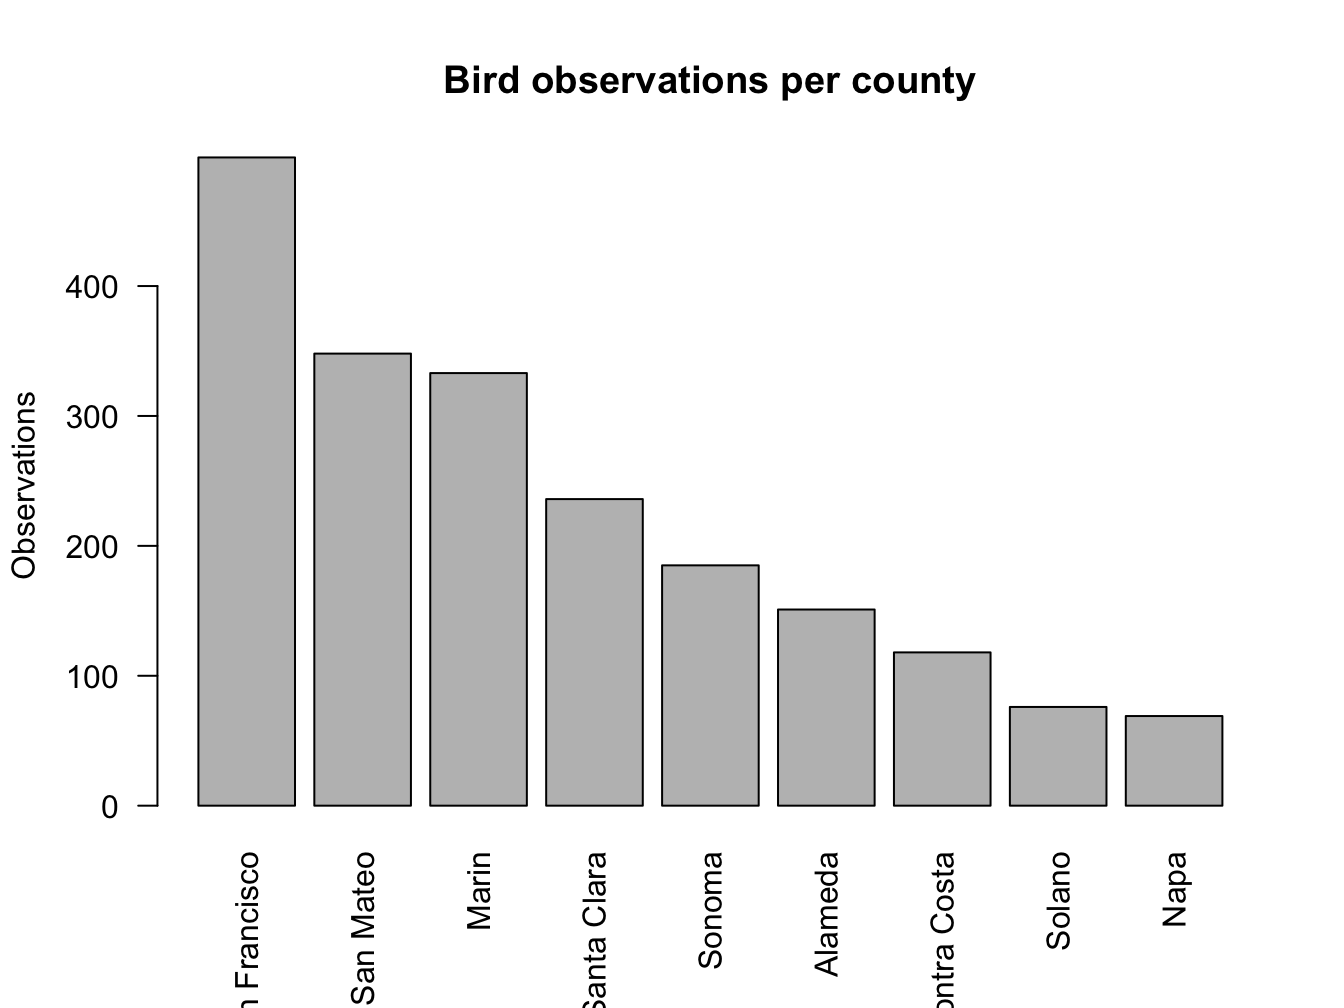
\includegraphics[width=0.8\linewidth]{davur_ebook_files/figure-latex/bird-counts-barplot-1} \end{center}

\textbf{B}

\begin{Shaded}
\begin{Highlighting}[]
\NormalTok{obs.split <-}\StringTok{ }\KeywordTok{split}\NormalTok{(}\DataTypeTok{x =}\NormalTok{ bird_obs, }\DataTypeTok{f =}\NormalTok{ bird_obs}\OperatorTok{$}\NormalTok{Observer}\FloatTok{.1}\NormalTok{)}
\NormalTok{obs.counts <-}\StringTok{ }\KeywordTok{sapply}\NormalTok{(obs.split, nrow)}
\NormalTok{obs.counts <-}\StringTok{ }\NormalTok{obs.counts[obs.counts }\OperatorTok{>}\StringTok{ }\DecValTok{10}\NormalTok{]}
\NormalTok{obs.counts[}\KeywordTok{order}\NormalTok{(obs.counts, }\DataTypeTok{decreasing =}\NormalTok{ T)]}
\end{Highlighting}
\end{Shaded}

\textbf{C}

\begin{Shaded}
\begin{Highlighting}[]
\NormalTok{obs.counts[}\KeywordTok{order}\NormalTok{(obs.counts, }\DataTypeTok{decreasing =}\NormalTok{ T)][}\DecValTok{1}\NormalTok{]}
\end{Highlighting}
\end{Shaded}

\textbf{D}

\begin{Shaded}
\begin{Highlighting}[]
\NormalTok{g.split <-}\StringTok{ }\KeywordTok{split}\NormalTok{(bird_obs, bird_obs}\OperatorTok{$}\NormalTok{Genus)}
\NormalTok{g.species <-}\StringTok{ }\KeywordTok{lapply}\NormalTok{(g.split, }\ControlFlowTok{function}\NormalTok{(x) \{}
        \KeywordTok{unique}\NormalTok{(x}\OperatorTok{$}\NormalTok{Common.name)}
\NormalTok{\})}
\CommentTok{#create ordering}
\NormalTok{g.species.count <-}\StringTok{ }\KeywordTok{sapply}\NormalTok{(g.species, length)}
\NormalTok{g.order <-}\StringTok{ }\KeywordTok{order}\NormalTok{(g.species.count, }\DataTypeTok{decreasing =}\NormalTok{ T)}
\CommentTok{#apply order to list and select only first five}
\NormalTok{g.species[g.order[}\DecValTok{1}\OperatorTok{:}\DecValTok{5}\NormalTok{]]}
\end{Highlighting}
\end{Shaded}

\textbf{E}

\begin{Shaded}
\begin{Highlighting}[]
\NormalTok{bird_obs}\OperatorTok{$}\NormalTok{Date.start <-}\StringTok{ }\KeywordTok{as.Date}\NormalTok{(bird_obs}\OperatorTok{$}\NormalTok{Date.start, }\DataTypeTok{format =} \StringTok{"%d-%b-%y"}\NormalTok{)}
\NormalTok{date.series <-}\StringTok{ }\KeywordTok{aggregate}\NormalTok{(Count }\OperatorTok{~}\StringTok{ }\NormalTok{Date.start, }\DataTypeTok{data =}\NormalTok{ bird_obs, }\DataTypeTok{FUN =}\NormalTok{ sum, }\DataTypeTok{na.rm =}\NormalTok{ T)}
\CommentTok{#2024 is an error input, remove it}
\NormalTok{date.series <-}\StringTok{ }\NormalTok{date.series[}\DecValTok{1}\OperatorTok{:}\KeywordTok{nrow}\NormalTok{(date.series)}\OperatorTok{-}\DecValTok{1}\NormalTok{, ]}
\KeywordTok{plot}\NormalTok{(}\DataTypeTok{x =}\NormalTok{ date.series}\OperatorTok{$}\NormalTok{Date.start, }\DataTypeTok{y =}\NormalTok{ date.series}\OperatorTok{$}\NormalTok{Count, }\DataTypeTok{ylim =} \KeywordTok{c}\NormalTok{(}\DecValTok{0}\NormalTok{, }\DecValTok{250}\NormalTok{))}
\end{Highlighting}
\end{Shaded}

\bibliography{book.bib,packages.bib}


\end{document}
